\documentclass[12pt,a4paper]{article}

\usepackage{url}
\usepackage{amsmath}
\usepackage{amssymb}
\usepackage{amsthm}
\usepackage{array}
\usepackage{enumerate}
\usepackage{relsize}
\usepackage{algorithm}
\usepackage{algpseudocode}
\usepackage{parskip}
\usepackage{graphicx}
\usepackage[natbibapa]{apacite}
\usepackage{xcolor}
\usepackage{caption}
\usepackage{float}
\usepackage{setspace}
\usepackage{tabularx}
\usepackage[capitalise,noabbrev]{cleveref}
\usepackage{enumitem}
\graphicspath{{images/}}

\usepackage[
  top    = 2.75cm,
  bottom = 3.00cm,
  left   = 2.50cm,
  right  = 2.50cm
]{geometry}

\captionsetup{font=footnotesize,justification=justified,margin=2cm}
\onehalfspacing
\newcolumntype{Y}{>{\centering\arraybackslash}X}

\algnewcommand\algorithmicinput{\textbf{Input:}}
\algnewcommand\algorithmicoutput{\textbf{Output:}}
\algnewcommand\algorithmicsideeffect{\textbf{Side Effect:}}
\algnewcommand\Input{\item[\algorithmicinput]}
\algnewcommand\Output{\item[\algorithmicoutput]}
\algnewcommand\SideEffect{\item[\algorithmicsideeffect]}
\algnewcommand{\IIf}[1]{\State\algorithmicif\ #1\ \algorithmicthen}
\algnewcommand{\IIEf}[2]{\State\algorithmicif\ #1\ \algorithmicthen\ #2\ \algorithmicelse}
\newcommand{\compatible}{\smile}
\newcommand{\leafset}{\Lambda}
\newcommand{\weight}{\omega}
\newcommand{\TA}{T_\alpha}
\newcommand{\TB}{T_\beta}

\title{A Faster Construction of Frequency Difference Consensus Trees\\CG4001 Final Report}
\author{Varun Gupta\\A0147924X}

\newtheorem{incompatibility}{Lemma}
\newtheorem{freqdiffruntimecomponents}[incompatibility]{Corollary}
\newtheorem{lca}[incompatibility]{Lemma}
\newtheorem{linearrmq}[incompatibility]{Lemma}
\newtheorem{mergetrees}[incompatibility]{Lemma}
\newtheorem{cfddatastructure}[incompatibility]{Lemma}
\newtheorem{cfdquery}[incompatibility]{Lemma}
\newtheorem{rmqdatastructure}[incompatibility]{Lemma}
\newtheorem{rmqquery}[incompatibility]{Theorem}
\newtheorem{assocnode}[incompatibility]{Lemma}
\newtheorem{labelclusterscorrectness}[incompatibility]{Lemma}
\newtheorem{labelclustersidbounds}[incompatibility]{Lemma}
\newtheorem{labelclustersruntime}[incompatibility]{Lemma}
\newtheorem{weightingruntime}[incompatibility]{Lemma}
\newtheorem{findcovererrecursive}[incompatibility]{Lemma}
\newtheorem{mincoverrecursive}[incompatibility]{Lemma}
\newtheorem{findcovererruntime}[incompatibility]{Lemma}
\newtheorem{incompatibilitymincover}[incompatibility]{Lemma}
\newtheorem{updateincompatibleruntime}[incompatibility]{Lemma}
\newtheorem{impurenodesincompatible}[incompatibility]{Lemma}
\newtheorem{restrictedrmq}[incompatibility]{Lemma}
\newtheorem{numremovednodesrecursive}[incompatibility]{Lemma}
\newtheorem{numremovednodescentroid}[incompatibility]{Lemma}
\newtheorem{numremovednodesdummy}[incompatibility]{Lemma}
\newtheorem{numremovednodes}[incompatibility]{Lemma}
\newtheorem{numaddednodes}[incompatibility]{Lemma}
\newtheorem{incompatibilityrecursive}[incompatibility]{Lemma}
\newtheorem{filterclustersruntime}[incompatibility]{Lemma}
\newtheorem{freqdiffruntime}[incompatibility]{Theorem}


\begin{document}
    \pagenumbering{roman}
    \begin{titlepage}
        \begin{center}
            \Large
            \textbf{A Faster Construction of Frequency Difference Consensus Trees}

            \vspace{7cm}

            Submitted by\\
            Varun Gupta

            \vfill

            In partial fulfilment of the\\
            requirements for the Degree of\\
            Bachelor of Engineering (Computer Engineering)\\
            National University of Singapore
        \end{center}
    \end{titlepage}
    \newpage

    \begin{titlepage}
        \begin{center}
            \large
            B.Eng. Dissertation
            \vspace{2cm}

            \Large
            \textbf{A Faster Construction of Frequency Difference Consensus Trees}

            \vspace{4cm}

            \large
            By\\
            Varun Gupta\\
            National University of Singapore\\
            2018/2019
        \end{center}

        \vfill

        \large
        Project ID: H045660\\
        Project Supervisor: Dr. Wing-Kin Sung\\

        Deliverables:\\
        \hspace*{1.5cm}Report: 1 Volume
    \end{titlepage}
    \newpage

    \section*{Abstract}
    A consensus tree is used to summarise the branching information present in a set of phylogenetic trees. A number of ways of constructing consensus trees have been proposed; this report focuses on the frequency difference consensus tree. It presents a new deterministic algorithm for constructing this. Given $k$ phylogenetic trees with identical leaf label sets of size $n$, this algorithm constructs the frequency difference consensus tree in $O(kn\,log\,n)$ time, bettering the previously best known time of $O(kn\,log^2n)$.

    \vspace{1cm}
    Subject Descriptors:
    \begin{description}[labelindent=1cm]
        \item[F.2.2] Nonnumerical Algorithms and Problems---Computations on discrete structures
    \end{description}

    \vspace{0.5cm}
    Keywords:\\[0.2cm]
    \hspace*{1cm}Consensus trees, Algorithms, Bioinformatics

    \vspace{0.5cm}
    Implementation Software and Hardware:\\[0.2cm]
    \hspace*{1cm}MacOSX, C++, Boost
    \newpage

    \section*{Acknowledgements}

    \doublespacing
    This report concludes a four year long journey that has been in turns incredibly rewarding and immensely frustrating. As I approach the end of my undergraduate degree, it would be remiss of me to fail to thank the following individuals, without whom it would have been impossible for me to get through this.

    Firstly, my supervisor, Dr. Wing-Kin Sung, who guided me through every step of the project. Without his willingness to help, his eye for detail and his unstinting commitment to making this project the best version of itself possible, I would have been totally lost.

    Second, my friends - Srishti, whose maturity has ever been my anchor; Advay, whom I should have long since appointed as my official decision maker; Chandraanshu, who soaked up innumerable rants with nary a complaint; Avnika and Ishanee, who continue to tolerate me for reasons unknown; Shailesh, Akshat and Tanvi, who play the best game of cards I have seen; Archana, who is probably only joking about poisoning me; Pankaj, whose boundless enthusiasm is an instant pick-me-up; and all the rest, with whom countless memories were made.

    Finally, my parents, who believed in me even when I lost all faith and my sister, who has the uncanny ability to cheer me up no matter what.
    \newpage

    \onehalfspacing
    \tableofcontents
    \newpage

    \listoffigures
    \listoftables
    \newpage

    \pagenumbering{arabic}
    \section{Introduction}
    \label{sec:introduction}

    A \textit{taxon} (pl. taxa) is a group of organisms that taxonomists classify as a single unit, such as \textit{homo sapiens}. These come together to give a \textit{rooted phylogenetic tree}, which presents the evolutionary relationships between various taxa in a hierarchical manner. Each leaf in this tree represents a taxon. An internal node then represents the common ancestor of a subgroup of the taxa shown in the entire tree. Children of each node split the group rooted at that node into smaller ones. A subgroup of taxa that are descendants of some common ancestor is called a \textit{clade}, i.e. a clade is the leaf set of any node in a phylogenetic tree.

    We often obtain multiple phylogenetic trees from biological datasets. These trees may be produced from different datasets or from a single dataset using techniques like maximum parsimony that yield a number of candidate trees \citep{bryant1997hunting}. This motivates the concept of a \textit{consensus tree}, which reconciles many phylogenetic trees by summarising the branching information contained in each into a single tree. Consensus trees are also useful in determining which clades have strong suppport within the input trees \citep{felsenstein2004inferring}.

    A variety of techniques of constructing a consensus tree from a set of phylogenetic trees have been developed over the last half century, starting with the Adams consensus tree \citep{adams1972consensus} in 1972. There is strong motivation for the development of different types of consensus trees since they each have their own benefits and drawbacks. Some of these techniques are summarised in \S 6.2 of \cite{bryant1997hunting} and a comparative analysis can be found in \cite{bryant2003classification}. We discuss some of the techniques here. The \textit{strict consensus tree} \citep{sokal1981taxonomic} only keeps those clades that occur in all the input trees. While easily reconstructed and interpreted, it can discard a lot of potentially important information if there is a lot of disagreement between the various trees. The \textit{majority rule consensus tree} \citep{margush1981consensusn} is a generalisation of the previous, allowing all clades that occur in a majority of the trees. \cite{holder2008justification} showed that these trees are optimal given a certain context.

    This article studies a specific type of consensus tree, known as the \textit{frequency difference consensus tree} \citep{goloboff2003improvements}. The \textit{frequency difference consensus tree} (abbreviated henceforth as FDCT) further generalises the \textit{majority rule consensus tree}, keeping every clade that occurs in more trees than the most frequent clade that contradicts it (the concept of contradiction is formalized in Subsection~\ref{subsec:def}). The FDCT is motivated by a desire to design an effective criterion for determining which clades are strongly supported within a set of trees. As set out in \cite{goloboff2003improvements}, although the \textit{majority rule consensus tree} includes a clade that is supported by 60\% of a set of trees and contradicted by 40\% of them, it does not include a clade supported by 40\% of the trees but not contradicted by any of them. A possible resolution to this is to define strongly supported clades as those with greater frequency than all clades incompatible with them. These are called frequency difference clades and all of these are included in the FDCT.

    \cite{dong2010majority} provided a comparison of the FDCT and a few other types of consensus trees. \cite{barrett2013plastid} employed the idea of using frequency difference as a measure of clade support while analysing angiosperm phylogeny and commented ``[the] frequency difference metric ... is particularly useful for assessing support when it is not overwhelmingly in favour of one particular topology, and should be especially useful in phylogenomic analyses in general, where hundreds or thousands of characters may contribute to branch support''. \cite{steel2014axiomatic} investigated a generalisation of the FDCT to \textit{supertrees}, i.e. consensus trees built from input trees that do not necessarily have the same leaf sets. They show that, unlike some other popular techniques, the FDCT definition easily generalises to a viable supertree definition and conclude that the FDCT is ``worthy of more widespread usage and serious study''. Given that the FDCT and the frequency difference measure have been utilised in various studies over the years \citep{garcia2014testing,barrett2013plastid,molineri2010cladistic,molineri2013phylogeny,molineri2015phylogeny,lindqvist2006molecular,han2014new} and keeping in mind the favourable opinions above, we set out to improve upon the best known deterministic algorithm for reconstructing the FDCT of a set of trees.

    \subsection{Definitions and Notation}
    \label{subsec:def}

    We define a rooted phylogenetic tree to be a rooted, leaf-labelled tree where every internal node has 2 or more children and every leaf has a different label. Henceforth, we will simply refer to these as trees. Let $T$ be some tree. The set of nodes of $T$ is denoted by $V(T)$. For any node $u \in V(T)$, the \textit{parent} of $u$ (if it exists) is represented by $parent^T(u)$ and the set of its \textit{children} is represented by $children^T(u)$. The \textit{depth} of $u$, denoted by $depth^T(u)$ is the number of nodes that are its proper ancestors. A node that is \textit{shallower} than another has a smaller depth value. We also define, for any nodes $u, v \in V(T)$ where $v$ is an ancestor of $u$, the sets $path^T(u, v), path^T(u, v], path^T[u, v)$ and $path^T[u, v]$. Here, the parentheses and square brackets obey the accepted notation for open and closed intervals, such that $path^T(u, v)$ is the set of nodes on the path from $u$ to $v$, excluding both these nodes, $path^T[u, v]$ includes both $u$ and $v$ and so on.

    Let $\leafset^T$ be the set of leaf labels of $T$. Non-empty subsets of $\leafset^T$ are called \textit{clusters} (we use the term clusters instead of clades for consistency with recent literature). Clusters with cardinality $1$ or $|\leafset^T|$ are \textit{trivial clusters}. For any node $u \in V(T)$, $T[u]$ is the subtree of $T$ rooted at $u$ and $\leafset^T(u)$ is the leafset of $T[u]$, called the cluster \textit{associated} with $u$. For example, in Figure~\ref{fig:freqdiff}, the node labelled by $2$ in $T_1$ has the cluster $\{a, b\}$ associated with it. The \textit{cluster collection} of $T$, $\mathcal{C}(T)$ is the set $\bigcup_{u \in V(T) - \{root(T)\} - \leafset^T} {\leafset^T(u)}$, i.e. a set containing all non-trivial clusters in $T$. For example, the cluster collection of $T_2$ in Figure~\ref{fig:freqdiff} is $\{\{b, c\}, \{a, b, c\}, \{d, e\}\}$. Any cluster $C \subseteq \leafset(T)$ \textit{occurs} in $T$ iff $C \in \mathcal{C(T)}$. Also, for any nodes $u, v \in V(T)$, denote the lowest common ancestor of $u$ and $v$ in $T$ by $lca^T(u, v)$. Further, for any non-empty set of nodes $U \subseteq V(T)$, denote the lowest common ancestor of all these nodes in $T$ by $lca^T(U)$.

    Any two clusters $C_1, C_2 \subseteq \leafset(T)$ are said to be \textit{compatible}, denoted as $C_1 \compatible C_2$, iff $C_1 \subseteq C_2$ or $C_2 \subseteq C_1$ or $C_1 \cap C_2 = \emptyset$. If $C_1$ and $C_2$ satisfy none of the preceding properties, then they are said to be \textit{incompatible} (referred to as \textit{contradiction} in Section~\ref{sec:introduction}), denoted as $C_1 \not\compatible C_2$. Similarly, given trees $T_1$ and $T_2$ with identical leaf sets, and nodes $u \in V(T_1)$, $v \in V(T_2)$, we say $u$ is compatible with $v$, denoted as $u \compatible v$, if the clusters associated with $u$ and $v$ are compatible. For example (referring to Figure~\ref{fig:freqdiff}), let $u$ be the node in $T_1$ associated with the cluster $\{a, b\}$, $v$ the node in $T_2$ associated with $\{a, b, c\}$ and $w$ the node in $T_2$ associated with $\{b, c\}$. Then $u$ and $v$ are compatible since $\leafset^{T_1}(u) \subseteq \leafset^{T_2}(v)$. However, $u$ is incompatible with $w$ since they share $b$ but neither leafset is a subset of the other. We now extend the notion of compatibility to trees. A cluster $C \subseteq \leafset(T)$ is \textit{compatible} with $T$ (denoted as $C \compatible T$) iff for every $C_1 \in \mathcal{C}(T)$, $C \compatible C_1$. Further, two trees $T_1$ and $T_2$ with identical leafsets are \textit{compatible} (denoted as $T_1 \compatible T_2$) iff for every $C \in \mathcal{C}(T_1)$, $C \compatible T_2$, i.e. if every cluster in $T_1$ is compatible with $T_2$. Observe that this also means that every cluster in $T_2$ is compatible with $T_1$. Thus in Figure~\ref{fig:freqdiff}, $T_1$ is incompatible with $T_2$ since the former contains the cluster $\{a, b\}$ which is incompatible with $\{b, c\}$, contained in the latter tree (in fact, it can be checked that all the trees in this figure are incompatible).

    \begin{figure}[ht]
        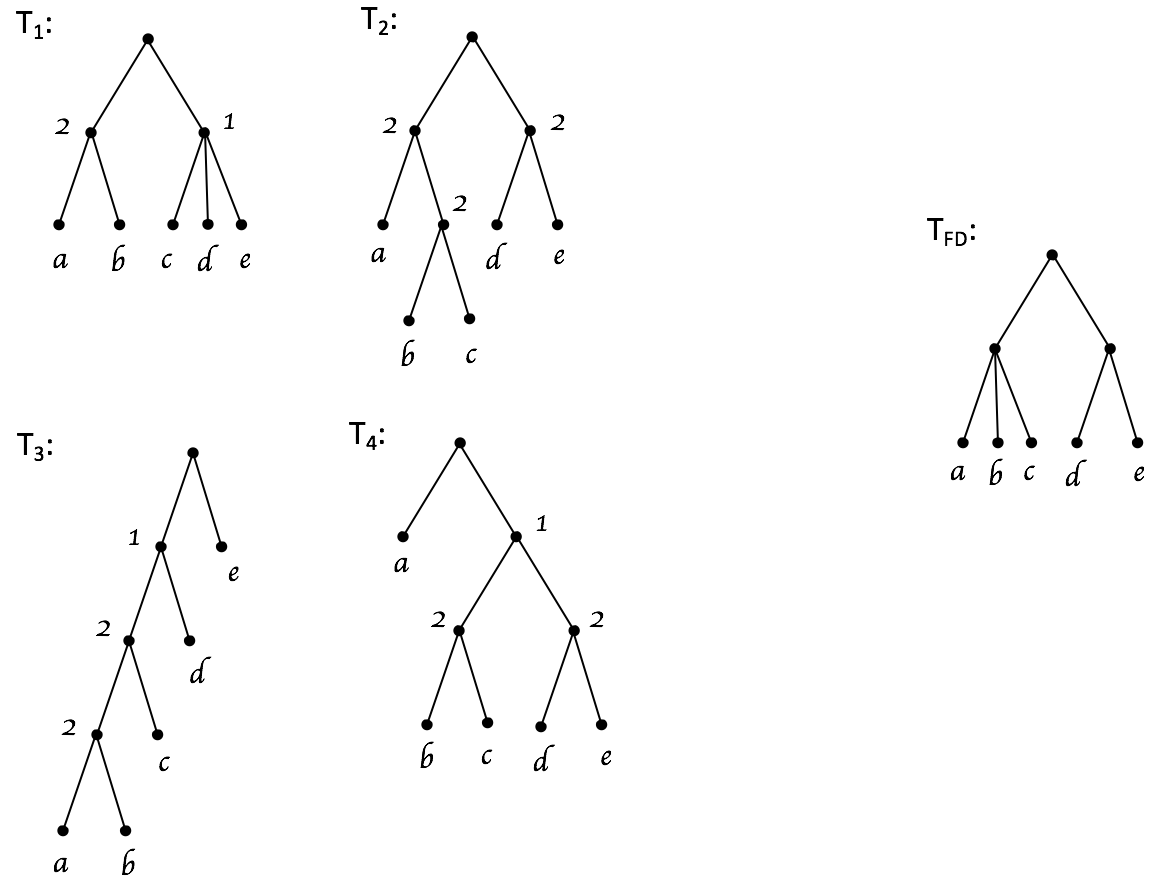
\includegraphics[scale=0.5]{freqdiff}
        \centering
        \caption[Example of a frequency difference consensus tree]{Let $\mathcal{S} = \{T_1, T_2, T_3, T_4\}$. $T_{FD}$ is the FDCT of $\mathcal{S}$. The number beside each non-root internal node $u$ indicates the weight of the node, $\weight(u)$, which is the number of occurences of the cluster $\leafset(u)$ in $\mathcal{S}$.}
        \label{fig:freqdiff}
    \end{figure}

    A \textit{frequency difference consensus tree} is defined as follows. Let $\mathcal{S}$ be a set of $k$ trees with identical leaf labels, i.e. $\mathcal{S} = \{T_1, T_2, ..., T_k\}$, where $\leafset(T_1) = \leafset(T_2) = ... = \leafset(T_k) = L$. For any cluster $C \subseteq L$, let weight of $C$, denoted as $\weight(C)$, be $|\{T : T \in \mathcal{S} \text{ and } C \in \mathcal{C}(T)\}|$, i.e. the number of trees in $\mathcal{S}$ which $C$ occurs in. For convenience, we also define, for any tree $T \in \mathcal{S}$, for any node $u \in V(T)$, the weight of $u$, denoted as $\weight(u)$ to be $\weight(\leafset^{T}(u))$. Then the FDCT of $\mathcal{S}$ is the tree $T_{FD}$, where $\mathcal{C}(T_{FD}) = \{C : C \subseteq L \text{ and } \weight(C) > max(\{\weight(C_1) : C_1 \subseteq L \text{ and } C \not\compatible C_1\})\}$. Thus $T_{FD}$ contains all clusters that occur more frequently than any cluster that they are incompatible with. By Proposition $3$ in \cite{steel2014axiomatic}, this tree always exists and is unique for a given $\mathcal{S}$. Figure~\ref{fig:freqdiff} gives an example. In this, $\weight(\{a, b\}) = 2 \leq \weight(\{b, c\}) = 2$ and $\{a, b\} \not\compatible \{b, c\}$, hence $\{a, b\}$ is not in the final consensus tree. However $\{a, b, c\}$ and $\{d, e\}$ have frequencies greater than any cluster incompatible with them, hence they both exist in the consensus tree. Note that frequencies are not shown for the trivial clusters.

    For each of the definitions above where the tree is specified in the superscript, this superscript is omitted if the tree being referred to is clear from context. For example, $children^T(u)$ would be written as $children(u)$. This will also be applied to any notation developed in the remainder of this text.

    Henceforth, $\mathcal{S}$ is taken to be the input set of trees with identical leaf labels. This set of leaf labels is denoted by $L$. Let $|\mathcal{S}| = k$ and $|L| = n$.

    \subsection{Previous Work}
    \label{subsec:previouswork}

    An implementation of the FDCT can be found in the free software package TNT \citep{goloboff2008tnt}; however the algorithm used within is unavailable and so its complexity is not known. \cite{jansson2018algorithms} gave a deterministic $min\{O(kn^2), O(kn(k + log^2 n))\}$ algorithm for constructing the FDCT, implemented in the open source FACT package \citep{jansson2016improved}. \cite{gawrychowski2017faster} improved upon this to give a deterministic $O(kn\,log^2n)$ algorithm (not yet implemented).

    \subsection{Organisation of the Article and New Results}
    Section~\ref{sec:preliminaries} contains some results from previous works that are utilised later. Sections~\ref{sec:cfd} and~\ref{sec:rmqtree} show how certain efficient data structures can be built on trees; these will be utilised later. Sections~\ref{sec:weighting} and~\ref{sec:filterclusters} present algorithms for solving subproblems of the FDCT construction; these are brought together in Section~\ref{sec:freqdiffconstruction} to give a new deterministic algorithm for constructing the FDCT that runs in $O(kn\,log\,n)$ time. Finally, Section~\ref{sec:implementation} details how the algorithm was implemented and presents some experimental results.

    \section{Preliminaries}
    \label{sec:preliminaries}

    \subsection{The \textit{lca} operation}

    We restate the following lemma outlining the \textit{lca} operation from \cite{bender2000lca}:
    \newline

    \begin{lca}
        \label{lem:lca}

        Given any tree $T$, the $lca$ data structure can be constructed in $O(n)$ time, where $n = |V(T)|$. Then, for any nodes $u, v \in V(T)$, the query $lca^{T}(u, v)$ can be answered in constant time.
    \end{lca}

    \subsection{The linear RMQ (range minimum/maximum) data structure}

    For any array $A[1 ... n]$ of length $n$ and any indices $i, j$, $1 \leq i \leq j \leq n$, let $rmq^A(i, j)$ denote $max_{i \leq k \leq j}A[k]$. We restate the following lemma about answering $rmq$ queries from \cite{bender2000lca}:
    \newline

    \begin{linearrmq}
        \label{lem:linearrmq}

        Given an array $A$ of numbers of length $n$, the \textit{linear RMQ data structure} can be constructed in $O(n)$ preprocessing time. Then for any indices $i, j$, $1 \leq i \leq j \leq n$, the query $rmq^A(i, j)$ can be answered in constant time.
    \end{linearrmq}

    \subsection{Centroid Path Decomposition}

    The \textit{centroid path decomposition technique} of \cite{cole2000n} is used to decompose a tree $T$ into a path from the root to some leaf and a set of disjoint subtrees. For any $u \in V(T)$, we define the \textit{heaviest child} of $u$, denoted by $heavyChild(u)$, to be the one with the largest leafset, with ties broken arbitrarily. The remaining children are called the \textit{side children} of $u$, denoted by $sideChildren(u)$. A \textit{centroid path} in $T$ is the path formed by starting at the root and at each point following the heaviest child. The centroid path is denoted by $\pi(T) = \langle p_{\gamma}, p_{\gamma - 1}, ..., p_1 \rangle$, where $p_{\gamma}$ is the root of $T$ and $p_1$ is a leaf. Removing the path $\pi(T)$ from $T$ results in a set of disjoint subtrees of $T$, where the root of each such subtree is a child of some node in $\pi(T)$. These trees are called the \textit{side trees} of $\pi(T)$, denoted by $\sigma(T)$. Also, for any node $u \in V(T)$, let $\sigma(u)$ be the set of trees rooted at $sideChildren(u)$, called the side trees \textit{associated} with $u$. Figure~\ref{fig:centroid}(a) demonstrates this decomposition. Here, the bold path from the root to leaf is the centroid path. When the dashed edges and the nodes contained in the centroid path are removed from the tree, the side trees remain. In particular, it can be seen that there are two side trees associated with the root, one containing just a single leaf, while the other is a larger tree.

    We further define a \textit{complete centroid path decomposition} for any tree $T$. Here, the normal centroid path decomposition is applied on $T$, and then each side tree is recursively decomposed. This results in a set of disjoint paths in $T$, denoted by $\mathcal{P}(T)$. We also assign each path $P_i \in \mathcal{P}(T)$ a depth, denoted as $depth^{T}(P_i)$, defined to be $1\, +$ depth of centroid path containing the parent of the root of $P_i$. Intuitively, if we build a tree from only the roots of the centroid paths while maintaining the same relative structure, then the depth of a centroid path would simply be the depth of its root in this new tree. Figure~\ref{fig:centroid}(b) applies complete centroid path decomposition on the same tree as before. The bold paths, along with the isolated leaves, are centroid paths. As can be seen, the large side tree that remained intact in Figure~\ref{fig:centroid}(a) has now been recursively decomposed. The depth of each centroid path is shown next to its root.

    \begin{figure}[ht]
        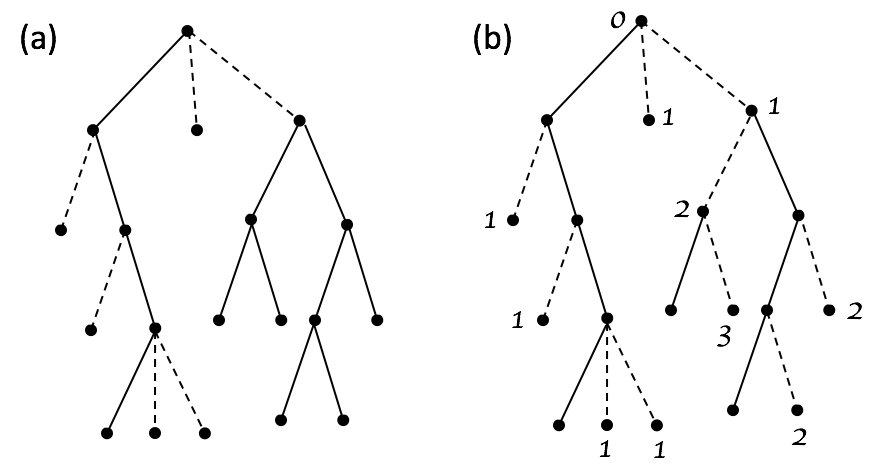
\includegraphics[scale=0.5]{centroid}
        \centering
        \caption[Centroid path decomposition]{Demonstration of centroid path decomposition. Both (a) and (b) use the same tree. In (a), the tree has undergone a centroid path decomposition such that after the dashed edges are removed, leaving a centroid path and a set of side trees. In (b), the tree has undergone a complete centroid path decomposition, with the dashed edges being removed to leave only a set of paths. The depth of each centroid path is shown next to its root.}
        \label{fig:centroid}
    \end{figure}

    \subsection{The \textit{delete} operation}
    \label{subsec:delete}

    As described in \cite{jansson2018algorithms}, the \textit{delete} operation deletes a cluster from a tree. To do so, we specify some internal node $u$ in a tree $T$, such that we wish to delete the cluster $\leafset^{T}(u)$. Then the \textit{delete} operation makes $parent(u)$ the parent of all nodes in $children(u)$ and removes $u$, along with any associated edges from $T$. This has the effect of removing only $\leafset(u)$ from $T$, without affecting any other cluster. For example, in Figure~\ref{fig:freqdiff}, if we perform a delete operation on $T_2$, on the node associated with the cluster $\{b, c\}$, the resulting tree is identical to $T_{FD}$.

    \subsection{Restricted Trees}
    \label{subsec:restrictedtree}

    For any tree $T$ and any cluster $C \subseteq \leafset(T)$, define $T|C$, read as ``$T$ restricted to $C$'', as the tree $T'$ with $V(T') = \{lca^T(u, v) : u, v \in C\}$ which obeys $lca^T(C') = lca^{T'}(C')$ for all $C' \subseteq C$. Intuitively, $T'$ has the leaf set $C$ and consists of all nodes in $T$ that are $lca$'s of the leaves in $C$, with these nodes connected such that they have the same ancestor/descendant relationships as they had in $T$. Figure~\ref{fig:restrictedtree} demonstrates this process. Notice that nodes which are not $lca$'s of the cluster are removed, but the structure of the tree in relation to the leaves in the cluster remains the same.

    \begin{figure}[ht]
        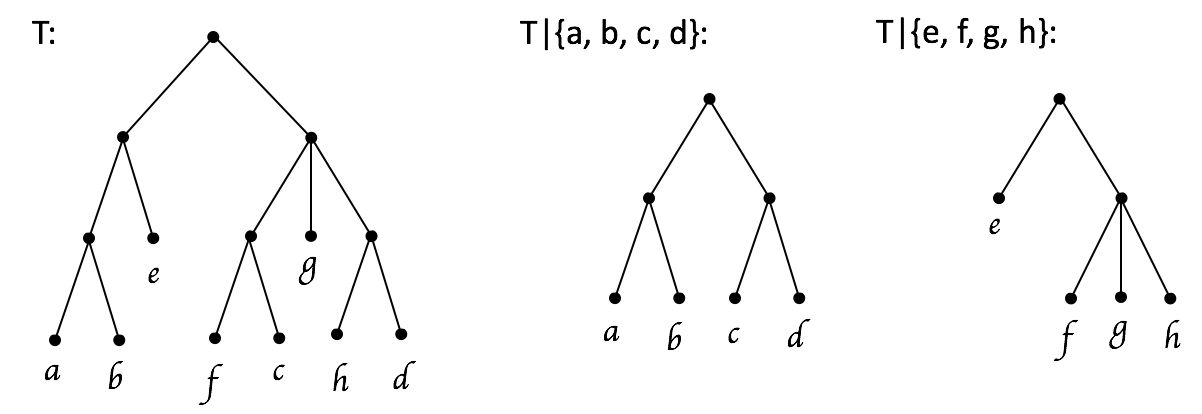
\includegraphics[scale=0.5]{restrictedsubtree}
        \centering
        \caption[Restricted Trees]{Illustration of restricting a tree to a cluster. The tree $T$, along with $T|\{a, b, c, d\}$ and $T|\{e, f, g, h\}$ are shown.}
        \label{fig:restrictedtree}
    \end{figure}

    \subsection{Characterising incompatibility}

    For any tree $T$ and cluster $C \subseteq \leafset(T)$, define the set $incompatible^{T}(C) = \{u : u \in V(T) \text{ and } \leafset^{T}(u) \not\compatible C\}$. Lemma 6 of \cite{jansson2018algorithms}, which gives a property of this set, is restated here since it is crucial in the development of an algorithm discussed below.
    \newline

    \begin{incompatibility}
        \label{lem:incompatibility}

        Given a tree $T$ and a cluster $C \subseteq \leafset(T)$, let $l_C = lca^T(C)$. Then for any $u \in V(T)$, $u \in incompatible^{T}(C)$ iff $u$ lies on the path between $l_C$ and some $x \in C$ and $\leafset(u) \not\subseteq C$.
    \end{incompatibility}

    \subsection{The \texttt{Merge\_Trees} algorithm}
    \label{subsec:mergetrees}

    We restate the following lemma outlining the \texttt{Merge\_Trees} operation from \cite{jansson2016improved}:
    \newline

    \begin{mergetrees}
        \label{lem:mergetrees}

        Given trees $T_1$ and $T_2$ where $\leafset^{T_1} = \leafset^{T_2} = L$ and $T_1 \compatible T_2$, \texttt{Merge\_Trees}$(T_1, T_2) = T$, where $\leafset^T = L$ and $\mathcal{C}(T) = \mathcal{C}(T_1) \cup \mathcal{C}(T_2)$. This algorithm runs in $O(|L|)$ time.
    \end{mergetrees}

    \begin{figure}[ht]
        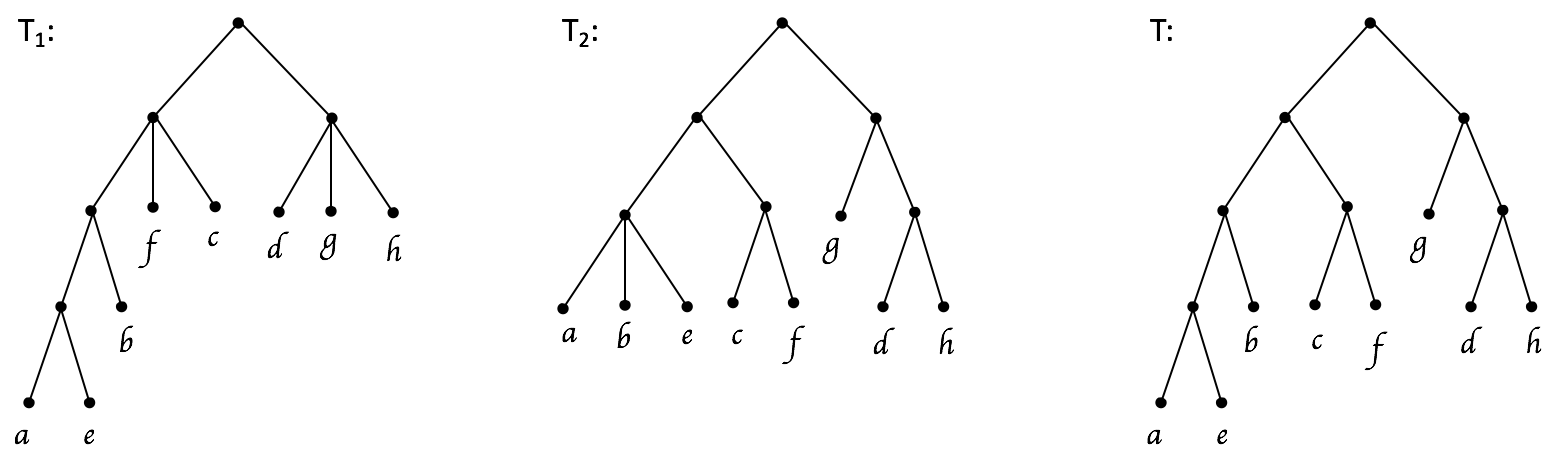
\includegraphics[scale=0.5]{mergetrees}
        \centering
        \caption[The \texttt{Merge\_Trees} algorithm]{$T_1 \compatible T_2$. $T =$ \texttt{Merge\_Trees}$(T_1, T_2)$. $\mathcal{C}(T) = \mathcal{C}(T_1) \cup \mathcal{C}(T_2)$.}
        \label{fig:mergetrees}
    \end{figure}

    Figure~\ref{fig:mergetrees} gives an example for the \texttt{Merge\_Trees} algorithm. Here, $T_1 \compatible T_2$ and $T =$ \texttt{Merge\_Trees}$(T_1, T_2)$. Observe that,
    \begin{align*}
        \mathcal{C}(T_1) &= \{\{a, e\}, \{a, b, e\}, \{a, b, c, e, f\}, \{d, g, h\}\}\\
        \mathcal{C}(T_2) &= \{\{a, b, e\}, \{c, f\}, \{a, b, c, e, f\}, \{d, h\}, \{d, g, h\}\}\\
        \mathcal{C}(T) &= \{\{a, e\}, \{a, b, e\}, \{c, f\}, \{a, b, c, e, f\}, \{d, h\}, \{d, g, h\}\}\\
        &= \mathcal{C}(T_1) \cup \mathcal{C}(T_2).
    \end{align*}

    \subsection{The \texttt{Frequency\_Difference} algorithm}

    The algorithm \texttt{Frequency\_Difference} \citep{jansson2018algorithms} computes the FDCT of a set of trees $\mathcal{S}$. It runs in two parts. First, for any tree $T \in \mathcal{S}$ and any node $u \in V(T)$, it computes $\weight(u)$ in the \textit{weighting} step. In the second part, it utilises \texttt{Filter\_Clusters} (defined below) and \texttt{Merge\_Trees} (from Subsection~\ref{subsec:mergetrees}) to compute the FDCT.

    As in \cite{jansson2018algorithms}, the subprocedure \texttt{Filter\_Clusters}, is defined to take as input trees $\TA$ and $\TB$, with $\leafset^{\TA} = \leafset^{\TB} = L$ and the values of $\weight(u)$ for all $u \in V(\TA) \cup V(\TB)$. It returns a tree $T$ which contains all clusters $C$ in $\TA$ for which $\weight(C) > $ weights of all clusters in $\TB$ that are incompatible with $C$. Formally, \texttt{Filter\_Clusters}$(\TA, \TB) = T$ where $\mathcal{C}(T) = \{C : C \in \mathcal{C}(\TA) \text{ and } \weight(C) > max(\{\weight(C_1) : C_1 \in \mathcal{C}(\TB) \text{ and } C_1 \not\compatible C\})\}$ and $\leafset^T = L$. For example, referring to Figure~\ref{fig:freqdiff}, \texttt{Filter\_Clusters}$(T_2, T_1) = T_{FD}$. Notice that there are three non-trivial clusters in $T_2$: $\{a, b, c\}, \{b, c\}$ and $\{d, e\}$. All of these have weight $2$. Now the only cluster in $T_1$ incompatible with $\{a, b, c\}$ is $\{c, d, e\}$, but this only has weight $1$ and so $\{a, b, c\}$ is kept. The cluster $\{d, e\}$ is compatible with $T_1$ so it is also kept. However, $\{b, c\}$ is incompatible with $\{a, b\}$ and they both have weight $2$, hence $\{b, c\} \not\in \mathcal{C}($\texttt{Filter\_Clusters}$(T_2, T_1))$.

    The \texttt{Frequency\_Difference} algorithm is given below.

    \begin{algorithm}
        \caption{Frequency\_Difference}
        \label{alg:frequencydifference}

        \begin{algorithmic}[1]
            \Input A set $\mathcal{S}$ of trees $\{T_1, T_2, ..., T_k\}$ where $\leafset(T_1) = \leafset(T_2) = ... = \leafset(T_k) = L$

            \Output A tree $T_{FD}$, where $\mathcal{C}(T_{FD}) = \{C : C \subseteq L \text{ and } \weight(C) > max(\{\weight(C_1) : C_1 \subseteq L \text{ and } C \not\compatible C_1\})\}$ and $\leafset^{T_{FD}} = L$.

            \State Compute $\weight(C)$ for every cluster $C$ that occurs in $S$.

            \State $T := T_1$

            \For{$j := 2$ to $k$}
                \State $A :=$ \texttt{Filter\_Clusters}$(T, T_j)$

                \State $B :=$ \texttt{Filter\_Clusters}$(T_j, T)$

                \State $T :=$ \texttt{Filter\_Clusters}$(A, B)$
            \EndFor

            \For{$j := 1$ to $k$}
                \State $T :=$ \texttt{Filter\_Clusters}$(T, T_j)$
            \EndFor

            \State \Return $T$
        \end{algorithmic}
    \end{algorithm}

    Theorem 3 of \cite{jansson2018algorithms} gives the following corollary:
    \newline

    \begin{freqdiffruntimecomponents}
        \label{cor:freqdiffruntimecomponents}

        The total runtime of \texttt{Frequency\_Difference} is given by $O(g(n, k) + k \cdot f(n))$ where $g(n, k)$ is the time taken by the weighting step and $f(n)$ is the runtime of \texttt{Filter\_Clusters}.
    \end{freqdiffruntimecomponents}

    \cite{jansson2018algorithms} gave a $min(\{O(kn^2), O(k^2n)\})$ solution to the weighting step and an $O(n\,log^2n)$ solution to \texttt{Filter\_Clusters}, giving an overall runtime of $min(\{O(kn^2), O(kn(k + log^2n))\})$. \cite{gawrychowski2017faster} improved the runtime of the weighting step to $O(kn\,log^2n)$, thus reducing the overall runtime to $O(kn\,log^2n)$.

    \section{$childD$ queries}
    \label{sec:cfd}

    Given a tree $T$ and nodes $v, w \in V(T)$ such that $w$ is a proper ancestor of $v$, define $childD(v, w)$ as the child of $w$ that is an ancestor of $v$. We construct a data structure that allows us to answer this query in constant time, given $O(n\,log\,n)$ preprocessing time, where $n = |V(T)|$.

    Reorder $T$ such that the heaviest child of each node is its leftmost child. Then the leaves of $T$ are indexed in left to right order, such that every leaf $x \in \leafset^T$ is assigned a value $index(x)$. Then for every node $u \in V(T)$, the indices of the leaves in $T[u]$ form a consecutive range. For each internal node $u \in V(T)$, define its side children to be the set $children(u) - \{\text{heaviest child of }u\}$ and its side trees to be the subtrees of $T$ rooted at its side children. Let $x$ and $y$ be the leaves in the side trees of $u$ with the smallest and largest indices respectively. We now build the array $cFL_u[0\, ...\, index(y) - index(x)]$ which maps each leaf $z$ in the side trees of $u$ to the child of $u$ that is an ancestor of $z$. Thus, for every leaf $z$ in $T[v]$ for some $v \in$ side children of $u$, let $cFL_u[index(z) - index(x)] = v$.
    \newline

    \begin{cfddatastructure}
        \label{lem:cfddatastructure}

        Given a tree $T$ where $n = |V(T)|$, the $cFL$ data structure defined above can be constructed in $O(n\,log\,n)$ time.

        \begin{proof}
            Rearranging $T$ and indexing the leaves can be done in two $O(n)$ passes. By the standard argument of centroid-path decomposition, we argue that any leaf is in the side trees of $O(log\,n)$ nodes, hence the total size of the $cFL$ arrays is $O(n\,log\,n)$. It is easy to see that these arrays can thus be constructed in $O(n\,log\,n)$ time.
        \end{proof}
    \end{cfddatastructure}

    \medskip
    \begin{cfdquery}
        \label{lem:cfdquery}

        Given a tree $T$, an $lca$ data structure on $T$, the $cFL$ data structure on $T$ and nodes $v, w \in V(T)$, the query $childD(v, w)$ can be answered in constant time.

        \begin{proof}
            The query is divided into two parts. First, we check if $v$ is a descendant of the heaviest child of $w$. If so, we are done. If not, we need to determine which child of $w$ is an ancestor of $v$.

            To answer the first part, we can see that, given nodes $r, s \in V(T)$, $s$ is an ancestor of $r$ iff $lca(r, s) = s$. Thus we can check if $v$ is a descendant of the heaviest child of $w$ in $O(1)$ time since by Lemma~\ref{lem:lca}, the $lca$ data structure allows queries in constant time.

            For the second part, we simply retrieve the entry corresponding to any leaf in $\leafset(v)$ from $cFL_w$, again easily done in constant time.
        \end{proof}
    \end{cfdquery}

    \section{RMQ structure on trees}
    \label{sec:rmqtree}

    Here, we generalise the linear RMQ data structure to trees. Given a tree $T$ and $\weight(u)$ for each $u \in V(T)$, for any nodes $v, w \in V(T)$ such that $w$ is an ancestor of $v$, let $rmqTree^T[v, w] = max_{u \in path^T[v, w]}\weight(u)$. Note that the square brackets are again used to indicate inclusion of the two endpoints. We build a data structure for answering $rmqTree^T[v, w]$ queries in constant time, given $O(n\,log\,n)$ preprocessing time, where $n = |V(T)|$.

    The data structure outlined here builds on the one presented in Lemma 8 of \cite{jansson2018algorithms}, while providing some further details of the implementation. We do a complete centroid path decomposition on $T$. Then for each leaf $x \in \leafset^T$, the path from $x$ to the root of $T$ can be seen as a concatenation of subpaths of centroid paths in $\mathcal{P}(T)$. An example of this can be seen in Figure~\ref{fig:rmq}. This figure shows part of a tree. The diagonal lines from right to left are centroid paths in the tree (elements of $\mathcal{P}(T)$). The dashed edges indicate that the child is not the heaviest child of its parent, hence starting a new centroid path. As can be seen, the path from the leaf $x$ to the root consists of subpaths of many centroid paths. The data structure we build consists of two parts. Firstly, for each centroid path $P_i \in \mathcal{P}(T)$, the weights along $P_i$ are stored in a linear RMQ structure (as described in Lemma~\ref{lem:linearrmq}). Secondly, for each $x$, we denote the subpaths of centroid paths on the leaf-root path by $Q_1, Q_2, ..., Q_f$, where $Q_1$ contains $root(T)$ and $Q_f$ contains $x$. Then we build the array $W_x[1 ... f]$, where $W_x[i] = max_{u \in Q_i} \weight(u)$ and store this array in a linear RMQ structure.
    \newline

    \begin{figure}[ht]
        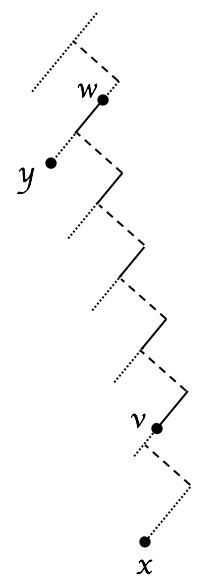
\includegraphics[scale=0.5]{rmq}
        \centering
        \caption[$rmqTree$ query]{Demonstration of an $rmqTree[v, w]$ query. The diagonal lines from right to left are centroid paths of the tree. The parts in bold lie on the path between $v$ and $w$, while those that are dotted do not. Dashed lines connect the root of a centroid path to its parent. $y$ is the leaf at the bottom of the centroid path to which $w$ belongs. $x$ is some leaf in the subtree rooted at $v$.}
        \label{fig:rmq}
    \end{figure}

    \begin{rmqdatastructure}
        \label{lem:rmqdatastructure}

        Given a tree $T$ and $\weight(u)$ for each $u \in V(T)$, the $rmqTree$ data structure can be built in $O(n\,log\,n)$ time.

        \begin{proof}
            The decomposition step, along with computation of depths for nodes and for centroid paths can be done in $O(n)$ time. Storing the centroid paths in linear RMQ structures takes $O(n)$ time, by Lemma~\ref{lem:linearrmq} and since the total size of the centroid paths is $O(n)$. By the standard argument of centroid-path decomposition, it can be seen that for each leaf $x$, the number of centroid subpaths on the path from the leaf to the root of $T$ is $O(log\,n)$. Hence it takes $O(log\,n)$ time to build the linear RMQ structure for these subpaths. Since there are $n$ leaves, the total time taken to construct the linear RMQ structures for all leaves is $O(n\,log\,n)$.
        \end{proof}
    \end{rmqdatastructure}

    \medskip
    \begin{rmqquery}
        \label{lem:rmqquery}

        Given a tree $T$, an $lca$ data structure on $T$, the $rmqTree$ data structure on $T$, and nodes $v, w \in V(T)$ such that $w$ is an ancestor of $v$, the query $rmqTree[v, w]$ can be answered in constant time.

        \begin{proof}
            We use the complete centroid path decomposition done when producing the $rmqTree$ data structure. The path from $v$ to $w$ is partitioned into a concatenation of subpaths of these centroid paths, denoted by $Q_1, Q_2, ..., Q_g$. This is illustrated in Figure~\ref{fig:rmq}. The diagonal lines from right to left are some of the centroid paths the tree has been decomposed into. The dashed edges indicate that the child is not the heaviest child of its parent, such that the child is the root of a new centroid path. The bold lines are the subpaths of centroid paths that lie on the path from $v$ to $w$. $Q_1$ is the bold centroid subpath starting from $v$ and continuing upwards till the root of that path. Similarly, $Q_g$ is the bold centroid subpath starting at $w$ and continuing downwards until the path splits from that centroid path. $Q_2$ to $Q_{g - 1}$ are the bold centroid subpaths between $Q_1$ and $Q_g$. The significance of the leaves $x$ and $y$ is explained below.

            Take any $x \in \leafset(v)$. Then $Q_2, ..., Q_{g - 1}$ are contained fully in the centroid subpaths on the path from $x$ to the root of $T$. $Q_1$ must be a subpath that starts at $v$ in some centroid path $\in \mathcal{P}(T)$ and ends at the root of that centroid path. $Q_g$ is a subpath that starts at some node in some centroid path $\in \mathcal{P}(T)$ and ends at $w$, within the same path. We address each of these three divisions separately.

            To find the maximum weight within $Q_1$, we obtain the depth of $v$ within $Q_1$ by subtracting the depth of the root of $Q_1$ from the depth of $v$. Then the maximum weight can be retrieved by querying the linear RMQ structure for this centroid path, from the root to $v$ (recall that the depths and linear RMQ structures were obtained while constructing the $rmqTree$ data structure). Querying the linear RMQ structure costs constant time, as set out in Lemma~\ref{lem:linearrmq}.

            To find the maximum weight for the subpaths $Q_2, ..., Q_{g - 1}$, we obtain the indices of $Q_2$ and $Q_{g-1}$ in $W_x$ as $depth^{T}(Q_1) + 1$ and $depth^{T}(Q_g) - 1$ respectively. The maximum weight can then be found by querying $W_x$.

            Finally, we need to find the maximum weight within $Q_g$. Observe that the key here is finding which node is at the end of $Q_g$. Let $P_i \in \mathcal{P}(T)$ be the centroid path of which $Q_g$ is a subpath. Then the previous question is equivalent to finding which node in $P_i$ has $v$ in one of its side trees. Let $y$ be the leaf at the bottom of $P_i$. Then the desired node is simply $lca(y, v)$, querying for which takes $O(1)$ time as given by Lemma~\ref{lem:lca}. The maximum weight within $Q_g$ can now be easily found in constant time by querying the linear RMQ structure for $P_i$, from $w$ to $lca(y, v)$.

            As of these three values can be obtained in constant time, the query as a whole takes $O(1)$ time.
        \end{proof}
    \end{rmqquery}

    \section{Weighting}
    \label{sec:weighting}

    Given the set of trees $\mathcal{S} = \{T_1, T_2, ..., T_k\}$, where $\leafset(T_1) = \leafset(T_2) = ... = \leafset(T_k) = L$ and $n = |L|$, the weighting step computes $\weight(u)$ for every node $u \in \bigcup_{T \in \mathcal{S}}V(T)$. Recall that $\weight(u)$ gives the frequency of $\leafset(u)$ in $\mathcal{S}$. We divide this work (as in \cite{gawrychowski2017faster}) into the labelling and counting steps. The labelling step assigns a label to each node $u \in T, T \in \mathcal{S}$, denoted by $id(u)$, such that $id(u) \in [1 ... 2kn]$ and for any node $u' \in T', T' \in \mathcal{S}$, $id(u) = id(u')$ iff $\leafset^T(u) = \leafset^{T'}(u')$. That is, two nodes have the same label iff they are associated with the same cluster. The counting step sorts these labels, allowing us to count how many nodes exist with each label, giving us the frequencies (or the weights) of the nodes.

    Recall that the approach in \cite{gawrychowski2017faster} costs $O(kn\,log^2n)$ time. We develop a way to achieve $O(kn\,log\,n)$ time.

    This problem can be solved using a divide and conquer strategy. Let\\ \texttt{Label\_Clusters}$(\{T_1, T_2, \dots, T_k\})$ be the procedure to compute the labels for all clusters. We partition $L$ into two equal sized halves, $L'$ and $L''$ such that $L = L' \cup L''$. Then we recursively call \texttt{Label\_Clusters}$(\{T_1|L', T_2|L', \dots, T_k|L'\})$ and\\ \texttt{Label\_Clusters}$(\{T_1|L'', T_2|L'', \dots, T_k|L''\})$. The first call gives us labels for the set of clusters $\{\leafset^{T|L'}(u) : T \in \mathcal{S}, u \in T|L'\}$, which turns out to be equivalent to the set $\{\leafset^{T}(u) \cap L' : T \in \mathcal{S}, u \in T\}$. Similarly, the second call gives labels for the set of clusters $\{\leafset^{T}(u) \cap L'' : T \in \mathcal{S}, u \in T\}$. Then for any tree $T \in \mathcal{S}$, for any node $u \in V(T)$, $\leafset^T(u)$ is uniquely identified by the pair $(id(\leafset^T(u) \cap L'), id(\leafset^T(u) \cap L''))$. To be able to quickly compute this pair, we introduce the definition below.

    Further, for every cluster $C \subseteq L$, and every node $u$ in $T$, define the node $assoc^C(u) = lca^T(C \cap \leafset^T(u))$. Notice that if $C \cap \leafset^T(u) \neq \emptyset$, $assoc^C(u) \in V(T|C)$ since it is the $lca$ of some non-empty subset of $C$. However, if $C \cap \leafset^T(u) = \emptyset$, then for convenience let $assoc^{C}(u) = \Phi$, where $\Phi$ is a special node with $id(\Phi) = 0$ and $\leafset(\Phi) = \emptyset$. We refer to Figure~\ref{fig:labelclusters} to show examples of this concept. Let $u$ and $v$ be the nodes in $T_1$ labelled $(5, 1)$ and $(5, 0)$ respectively. Then $assoc^{\{a, b, c, d\}}(u) = v$, since $v = lca^{T_1}(\{a, b, c, d\} \cap \leafset^{T_1}(u)) = lca^{T_1}(\{a, b\})$. $assoc^{\{e, f, g, h\}}(v) = \Phi$, since $\leafset^{T_1}(v) \cap \{e, f, g, h\} = \emptyset$.
    \newline

    \begin{labelclusterscorrectness}
        \label{lem:labelclusterscorrectness}

        Given any trees $T_i, T_j \in \mathcal{S}$, for any nodes $u \in V(T_i), v \in V(T_j)$,\\ $(id(assoc^{L'}(u)), id(assoc^{L''}(u))) = (id(assoc^{L'}(v)), id(assoc^{L''}(v)))$ iff $\leafset^{T_i}(u) = \leafset^{T_j}(v)$.

        \begin{proof}
            Inductively, $id(assoc^{L'}(u)) = id(assoc^{L'}(v))$ iff $\leafset^{T_i|L'}(assoc^{L'}(u)) = \leafset^{T_j|L'}(assoc^{L'}(v))$. By definition of the $assoc$ relation, $\leafset^{T_i}(u)\, \cap\, L' = \leafset^{T_j}(v)\, \cap\, L'$. Symmetrically, $id(assoc^{L''}(u)) = id(assoc^{L''}(v))$ iff $\leafset^{T_i}(u)\, \cap\, L'' = \leafset^{T_j}(v)\, \cap\, L''$. Since $L'$ and $L''$ partition $L$, both parts are true iff $\leafset^{T_i}(u) = \leafset^{T_j}(v)$.
        \end{proof}
    \end{labelclusterscorrectness}

    Using this observation, we can expand on the previous description of the algorithm. As mentioned above, we first obtain, for every $T \in \mathcal{S}$, for every node $u \in V(T)$, the pair $(id(assoc^{L'}(u)), id(assoc^{L''}(u)))$. Then we sort them and assign a rank to each unique pair; $id(u)$ is then the rank of the pair $(id(assoc^{L'}(u)), id(assoc^{L''}(u)))$. The resulting algorithm \texttt{Label\_Clusters} is laid out below.

    \begin{algorithm}
        \caption{Label\_Clusters}
        \label{alg:labelclusters}

        \begin{algorithmic}[1]
            \Input A set $\mathcal{S}$ of trees $\{T_1, T_2, \dots, T_k\}$ where $\leafset(T_1) = \leafset(T_2) = \dots = \leafset(T_k) = L$

            \Output Associate a label $id(u) \in [1 \dots 2k |L|]$ with every node $u$ in the trees in $\mathcal{S}$ such that for any two nodes $v, w$ in some trees in $\mathcal{S}$, $id(v) = id(w)$ iff $\leafset(v) = \leafset(w)$.

            \State Partition $L$ into $L'$ and $L''$ such that $|L'| = |L''|$.

            \State For all $i \in [1 \dots k]$, let $T'_i = T_i|L'$ and $T''_i = T_i|L''$.

            \State \texttt{Label\_Clusters}$(\{T'_1, T'_2, \dots, T'_k\})$.

            \State \texttt{Label\_Clusters}$(\{T''_1, T''_2, \dots, T''_k\})$.

            \State For every tree $T \in \mathcal{S}$, for every node $u \in T$, represent $u$ by the pair $(id(assoc^{L'}(u)), id(assoc^{L''}(u)))$.

            \State Radix sort all pairs obtained and remove duplicates. Assign a rank to each unique pair.

            \State For every tree $T \in \mathcal{S}$, for every node $u \in T$, set $id(u) = $ rank of the pair $(id(assoc^{L'}(u)), id(assoc^{L''}(u)))$.
        \end{algorithmic}
    \end{algorithm}

    One iteration of this process is illustrated in Figure~\ref{fig:labelclusters}. Here $L' = \{a, b, c, d\}$ and $L'' = \{e, f, g, h\}$. It is assumed that the algorithm has correctly labelled the clusters for each of the restricted trees, and these labels are assigned as shown in Figure~\ref{fig:labelclusters}(b). Figure~\ref{fig:labelclusters}(a) then shows the pair associated with each internal node of $T_1$ and $T_2$. For example, the cluster $\{a, b, e\}$ in $T_1$ is labelled by $5$ from $\{a, b\}$ in $T_1|L'$ and $1$ from $\{e\}$ in $T_1|L''$. Similarly, the cluster $\{a, b\}$ in $T_1$ is labelled by $5$ from $\{a, b\}$ in $T_1|L'$ and $0$ from $\Phi$ since $\{a, b\} \cap \{e, f, g, h\} = \emptyset$.

    \begin{figure}[ht]
        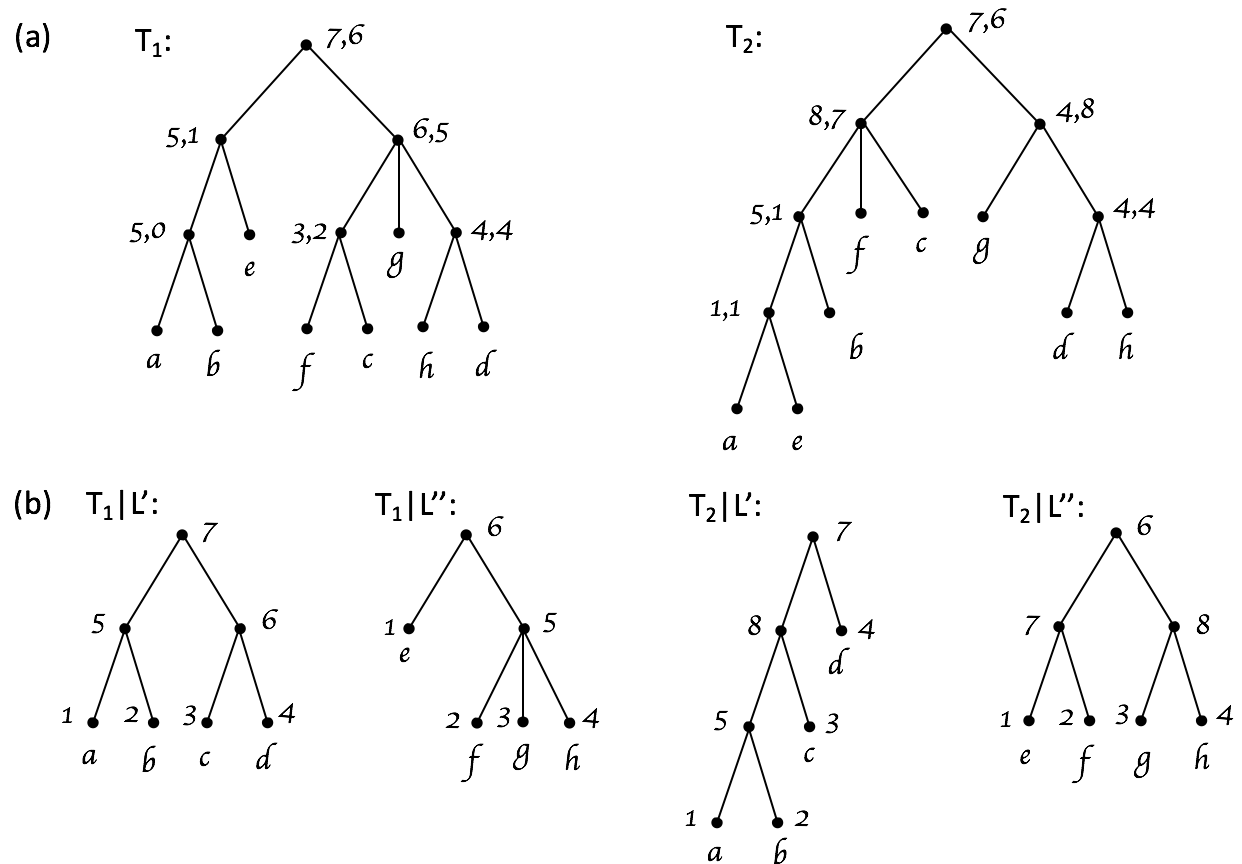
\includegraphics[scale=0.5]{labelclusters}
        \centering
        \caption[The \texttt{Label\_Clusters} algorithm]{Demonstration of \texttt{Label\_Clusters}$(T_1, T_2)$. $L' = \{a, b, c, d\}$ and $L'' = \{e, f, g, h\}$. (b) shows the trees $T_1|L', T_1|L'', T_2|L'$ and $T_2|L''$, where these have been recursively labelled. The labels are shown beside each of the nodes. (a) shows the trees $T_1$ and $T_2$ where the pair that represents each node (except the leaves) is shown beside it.}
        \label{fig:labelclusters}
    \end{figure}

    \bigskip
    \begin{labelclustersidbounds}
        \label{lem:labelclustersidbounds}

        After running \texttt{Label\_Clusters}$(\mathcal{S})$, for any node $u \in V(T), T \in \mathcal{S}$, $id(u) \in [1 \dots 2k |L|]$.

        \begin{proof}
            It is easily seen that $|V(T)| < 2|L|$. Thus the total number of pairs is less than $2k|L|$. This also places an upper bound on the number of ids. Notice that $u$ cannot be labelled with $0$ since that is reserved for the special node.
        \end{proof}
    \end{labelclustersidbounds}

    \medskip
    \begin{labelclustersruntime}
        \label{lem:labelclustersruntime}

        The algorithm \texttt{Label\_Clusters}$(\mathcal{S})$ runs in $O(kn\,log\,n)$ time.

        \begin{proof}
            Let $T(m)$ be the runtime of \texttt{Label\_Clusters}$(\mathcal{T})$, where $m =$ size of leaf set of each tree in $\mathcal{T}$. By Lemma 5.2 of \cite{farach1995fast}, construction of $T'_i$ and $T''_i$ takes $O(m)$ time for each $T_i \in \mathcal{T}$, taking total $O(km)$ time over all the trees. Computing $assoc^{L'}(u)$ and $assoc^{L''}(u)$ for each node $u$ in some tree $T_i \in \mathcal{T}$ can be done by a bottom up traversal of $T_i$ along with $T'_i$ and $T''_i$, taking $O(km)$ time total. Also observe that the number of pairs obtained is $O(km)$. Further, each of the values in the pair is in the range [0, km]. Thus radix sorting these pairs and assigning labels back to the nodes takes $O(km)$ time. So $T(m) = 2T(m/2) + O(km)$, giving $T(n) = kn\,log\,n$.
        \end{proof}
    \end{labelclustersruntime}

    \medskip
    \begin{weightingruntime}
        \label{lem:weightingruntime}

        The weighting step can be completed in $O(kn\,log\,n)$ time.

        \begin{proof}
            As shown in Lemma~\ref{lem:labelclustersruntime}, assigning labels to each node takes $O(kn\,log\,n)$ time. Next, we sort the labels by counting sort. Since each label is in the range $[1 ... 2kn]$ and there are $O(kn)$ labels, this takes $O(kn)$ time. The frequencies, or weights, can then be computed in $O(kn)$ time.
        \end{proof}
    \end{weightingruntime}

    \section{\texttt{Filter\_Clusters}}
    \label{sec:filterclusters}

    Given the trees $\TA$ and $\TB$ where $\leafset^{\TA} = \leafset^{\TB} = L$ and $n = |L|$, the algorithm\\ \texttt{Filter\_Clusters}$(\TA, \TB)$ returns a tree $T$, where $\mathcal{C}(T) = \{C : C \in \mathcal{C}(\TA) \text{ and } \weight(C) > max(\{\weight(C_1) : C_1 \in \mathcal{C}(\TB) \text{ and } C_1 \not\compatible C\})\}$ and $\leafset(T) = L$. Recall that the previous best known solution, as in \cite{jansson2018algorithms}, costs $O(kn\,log^2n)$ time; we present an $O(kn\,log\,n)$ solution.

    The key here is finding, for any node $u \in V(\TA)$, the set $incompatible^{\TB}(\leafset^{\TA}(u))$, so that we can find the maximum weight of the nodes in this set. Then it is easy to figure out whether $u$ should be in $T$ or not.

    Subsection~\ref{subsec:mincover} presents the definition $minCover^{T}(C)$. Subsection~\ref{subsec:redefiningincompatibility} uses this definition to give a stricter definition of incompatibility. Subsection~\ref{subsec:restrictedweighted} then presents the concept of weighted restricted trees. We then use all of these in Subsection~\ref{subsec:filterclusters} to create the algorithm \texttt{Filter\_Clusters}. Finally, Subsections~\ref{subsec:findcoverer} and~\ref{subsec:updateincompatible} prove two claims we make when analysing the runtime of \texttt{Filter\_Clusters}.

    \subsection{The concept of a \textit{minimum cover}}
    \label{subsec:mincover}

    Given a tree $T$ leaf-labelled by $L$ and a cluster $C \subseteq L$, define a set $M \subseteq V(T)$ to be a cover of $C$ in $T$ if $\bigcup_{u \in M} \leafset^{T}(u) = C$. Then we define the minimum cover of $C$ in $T$, denoted as $minCover^{T}(C)$, to be the smallest set $M$ such that $M$ is a cover of $C$. Note that this set is well defined for each cluster. Further, for any node $u \in V(T)$ such that $\leafset^{T}(u) \subseteq C$, define the node covering $u$, denoted as $coverer^{T, C}(u)$, to be the ancestor of $u$ which belongs to $minCover^{T}(C)$. Observe that this node must exist, since $\leafset^{T}(u)$ must be covered, and covering it with descendants of $u$ certainly yields a larger cover than if we use $u$. Figure~\ref{fig:mincoverrecursive}(a) gives an example of a minimum cover. In the same diagram, let $C = \{a, b, c, f, g, h\}$ and $u$ be as labelled. Then $coverer^{T, C}(u) = v$ and $minCover^{T}(C)$ is given by all the circled nodes.

    \begin{figure}[ht]
        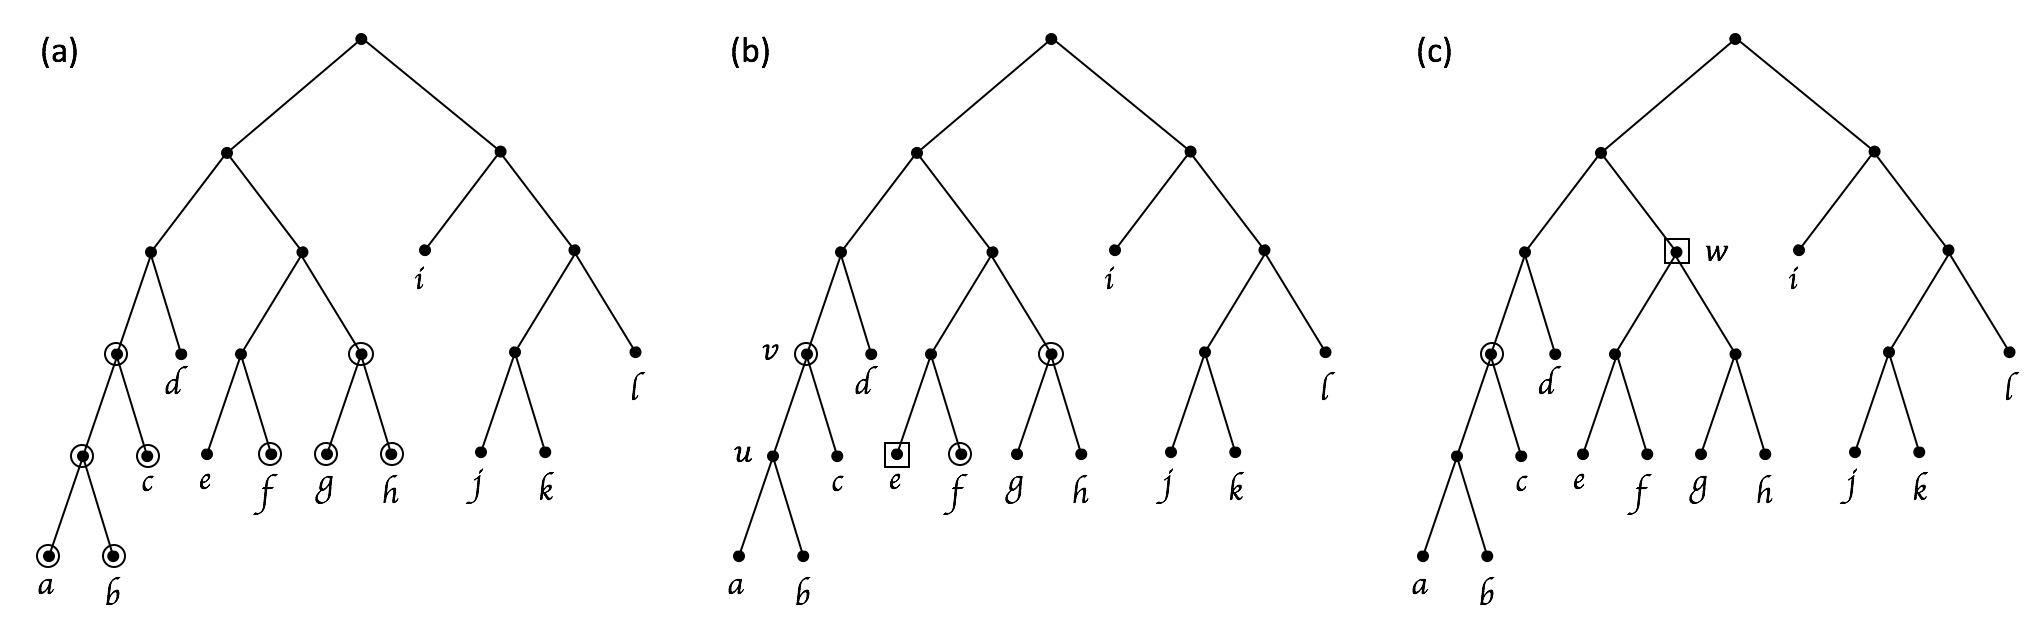
\includegraphics[scale=0.48]{mincoverrecursive}
        \centering
        \caption[Minimum cover and coverer]{Illustration of minimum cover and coverer. Let $C = \{a, b, c, f, g, h\}$. Then the circled nodes in (a) give $minCover^{T}(C)$. Take the leaf $e$, marked with a square in (a) and let $Ce = C \cup \{e\}$. Then $coverer^{T, Ce}(e) = w$, marked with a square in (b). Then the circled node and $w$ in (b) give $minCover^{T}(Ce)$.}
        \label{fig:mincoverrecursive}
    \end{figure}

    Given some tree $T$ leaf-labelled by $L$, cluster $C \subseteq L$ and node $u \in V(T)$ such that $\leafset^{T}(u) \cap C = \emptyset$, let $M = minCover^{T}(C)$ and $Cu = C \cup \leafset^{T}(u)$. Then it is useful to be able to find $coverer^{T, Cu}(u)$. Thus, we define the operation $findCoverer^{T, Cu}(u)$ which returns $coverer^{T, Cu}(u)$.

    Figure~\ref{fig:mincoverrecursive} demonstrates how this query works. Here, $C = \{a, b, c, f, g, h\}$ and we take the leaf $e$. The circled nodes in Figure~\ref{fig:mincoverrecursive}(a) give $minCover^{T}(C)$. Then we wish to compute $coverer^{T, Ce}(e)$, where $Ce = C \cup \{e\}$. The idea for doing so will be to iterate upwards from $e$ while the leafset of the node we are at is a subset of $Ce$. Thus, since $\leafset^{T}(parent(e)) \subseteq Ce$, we go upwards one level. We can then go a further  level, to the node $w$ since $\leafset^{T}(w) \subseteq Ce$. At this point we cannot go any further up. Hence, we say that we have found $w = coverer^{T, Ce}(e)$. This yields the following definition of $findCoverer^{T, Cu}(u)$:
    \newline

    \begin{findcovererrecursive}
        \label{lem:findcovererrecursive}

        Given a tree $T$ leaf-labelled by $L$, a cluster $C \subseteq L$ and a node $u \in V(T)$ such that $\leafset^{T}(u) \cap C = \emptyset$, let $M = minCover^{T}(C)$, $Cu = C \cup \leafset^{T}(u)$ and $v = parent(u)$. Then
        \[findCoverer^{T, Cu}(u) = \begin{cases}
            u & \leafset^{T}(v) \not\subseteq Cu\\
            findCoverer^{T, Cu}(v) & otherwise
        \end{cases}\]

        \begin{proof}
            \textit{Base Case.} If $\leafset^{T}(v) \not\subseteq Cu$, there is some leaf $x \in \leafset^{T}(v)$ such that $x \not\in C$. Thus $v$ cannot cover $\leafset^{T}(u)$, so $u = coverer^{T, Cu}(u)$.

            \textit{Inductive Case.} Since $v = parent(u)$ and $\leafset^{T}(v) \subseteq Cu$, $coverer^{T, Cu}(u) = coverer^{T, Cu}(v)$ so the algorithm works recursively. Also observe that the recursion has to terminate since in each recursive call we go one node further up the tree.
        \end{proof}
    \end{findcovererrecursive}

    Now given $coverer^{T, Cu}(u)$, we would like to actually obtain the minimum cover of $Cu$. Referring back to Figure~\ref{fig:mincoverrecursive}, notice that we can subtract the set of all children of the nodes on the path from $e$ to $w$ (excluding $e$) from $M$, add $w$, and this gives us the required set. That is, we take $M \cup \{w\} - \bigcup_{w' \in path^{T}(e, w]} children(w')$. This leads to the following lemma:
    \newline

    \begin{mincoverrecursive}
        \label{lem:mincoverrecursive}

        Given a tree $T$ leaf-labelled by $L$, a cluster $C \subseteq L$ and a node $u \in V(T)$ such that $\leafset^{T}(u) \cap C = \emptyset$ let $M = minCover^{T}(C)$, $Cu = C \cup \leafset^{T}(u)$ and $v = coverer^{T, Cu}(u)$. Then
         \[minCover^{T}(Cu) = M \cup \{v\} - \bigcup_{w \in path^{T}(u, v]} children(w)\]

        \begin{proof}
            Firstly, $M \cup \{v\} - \bigcup_{w \in path^{T}(u, v]} children(w)$ covers $Cu$. To see this, take any leaf $x \in Cu$. Then if $x \in \leafset^{T}(v)$, then we are clearly done. Otherwise, $x \in C$, so there must be some $c \in M$ such that $x \in leafset^{T}(c)$. But $c \not\in \bigcup_{w \in path^{T}(u, v]} children(w)$, otherwise $x \in \leafset^{T}(v)$. Thus $c \in M - \bigcup_{w \in path^{T}(u, v]} children(w)$, so we are done.

            Further, this must also be the minimum cover of $Cu$. Clearly, $v$ provides the smallest cover for $\leafset^{T}(v)$, which encapsulates $\leafset^{T}(u)$. Then if there is a smaller cover for $Cu$, we can cut and paste this into $M$, giving a smaller cover for $C$, which contradicts the definition of $M$.

            Thus we have the minimum cover for $Cu$.
        \end{proof}
    \end{mincoverrecursive}

    Subsection~\ref{subsec:findcoverer} details how to actually implement the \texttt{Find\_Coverer} operation. We now make a claim (proved later) about its running time.
    \newline

    \begin{findcovererruntime}
        \label{lem:findcovererruntime}

        Given a tree $T$ leaf-labelled by $L$, a cluster $C \subseteq L$ and a node $u \in V(T)$ such that $\leafset^{T}(u) \cap C = \emptyset$, let $M = minCover^{T}(C)$, $Cu = C \cup \leafset^{T}(u)$ and $v = coverer^{T, Cu}(u)$. Then the operations $findCoverer^{T, Cu}(u)$ can be performed in $O(|path^{T}(u, v]| + 1)$ time.

        \begin{proof}
            Proved in Subsection~\ref{subsec:findcoverer}.
        \end{proof}
    \end{findcovererruntime}

    \subsection{Redefining incompatibility}
    \label{subsec:redefiningincompatibility}

    With the concept of a minimum cover in hand, we can proceed to give a method to compute incompatibility. Given a tree $T$ and a cluster $C \subseteq L$, recall that the set $incompatible^{T}(C) = \{v : v \in V(T) \text{ and } \leafset^{T}(v) \not\compatible C\}$.
    \newline

    \begin{incompatibilitymincover}
        \label{lem:incompatibilitymincover}

        Given a tree $T$ leaf-labelled by $L$ and a cluster $C \subseteq L$, let $l_C = lca^{T}(C)$. Then for any node $u \in V(\TB)$, $u \in incompatible^{T}(C)$ iff $u$ is a proper ancestor of some node $c \in minCover^{T}(C)$ and $u$ is a proper descendant of $l_C$. In other words, $incompatible^{T}(C) = \bigcup_{c \in minCover^{T}(C)} path(c, l_C)$.

        \begin{proof}
            $\longrightarrow$. Given any $u \in V(T)$ such that $u \in incompatible^{T}(C)$, $u$ is a proper descendant of $l_C$ as a direct consequence of Lemma~\ref{lem:incompatibility}. Further, there is some leaf $x \in C$ such that $u$ is a proper ancestor of $x$ by Lemma~\ref{lem:incompatibility}. Then there must be some node $c \in V(T)$ such that $c$ is an ancestor of $x$ and $c \in minCover^{T}(C)$, otherwise $x$ would not be covered. If $c$ is an ancestor of $u$, then $\leafset^{T}(u) \subseteq \leafset^{T}(c) \subseteq C$, thus $\leafset^{T}(u) \compatible C$, which leads to a contradiction. Hence, $u$ is a proper ancestor of $c$.

            $\longleftarrow$. Given any $u \in V(T)$ such that $u$ is a proper ancestor of some node $c \in minCover^{T}(C)$ and $u$ is a proper descendant of $l_C$, $C \not\subseteq \leafset^{T}(u)$, since $u$ is a proper descendant of $l_C$. As $u$ is a proper ancestor of $c$, $\leafset^{T}(c) \subset \leafset^{T}(u)$. Also, $\leafset^{T}(c) \subset C$ by the definition of minimum cover. Thus $\leafset^{T}(u) \cap C \neq \emptyset$. Also, if $\leafset^{T}(u) \subseteq C$, we could create a smaller cover for $C$ by removing all proper descendants of $u$ from $minCover^{T}(C)$ and adding $u$. Note that this would give a smaller cover as there must be more than one such proper descendant of $u$, since $c$ is a proper descendant of $u$ and $\leafset^{T}(c) \subset C$. Hence, $u \in incompatible^{T}(C)$.
        \end{proof}
    \end{incompatibilitymincover}

    The above result is illustrated in Figure~\ref{fig:incompatibility}(a).

    \begin{figure}[ht]
        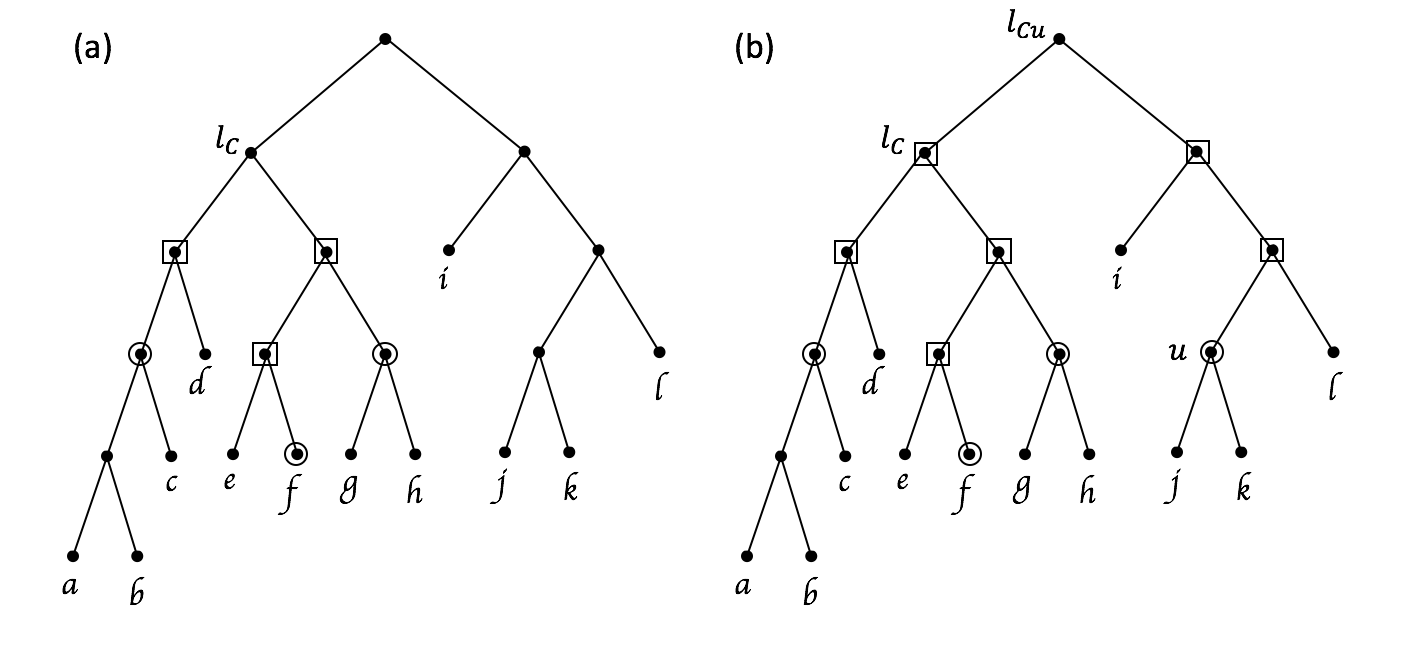
\includegraphics[scale=0.5]{incompatibility}
        \centering
        \caption[Incompatibility and the $updateIncompatible$ operation]{Illustration of Lemma~\ref{lem:incompatibilitymincover} and an $updateIncompatible$ operation. Let $C = \{a, b, c, f, g, h\}$. Then in (a), $l_C = lca^T(C)$, the circled nodes give $minCover^{T}(C)$ and the nodes marked with squares give $incompatible^T(C)$. Notice that all nodes in $incompatible^T(C)$ are proper descendants of $l_C$ and proper ancestors of some $c \in minCover^{T}(C)$. Referencing (b), let $Cu = C \cup \leafset^{T}(u)$ and $l_{Cu} = lca^{T}(Cu)$. Note that $u = coverer^{T, Cu}(u)$. Then we run $updateIncompatible^{T}(incompatible^{T}(C), u, u, l_C, l_{Cu})$. Again, nodes in $minCover^{T}(Cu)$ are circled and nodes in $incompatible^{T}(Cu)$ are marked with squares.}
        \label{fig:incompatibility}
    \end{figure}

    We now wish to define an operation which takes the set of nodes incompatible with a given cluster and updates this set to become those incompatible with a superset of that cluster. Formally, given tree a $T$ leaf-labelled by $L$, a cluster $C \subseteq L$ and a node $u \in V(T)$ such that $\leafset^{T}(u) \cap C = \emptyset$, we would like to have an operation that takes in $I$ and $u$ (along with some other arguments) and returns $incompatible^{T}(C \cup \leafset^{T}(u))$. Figure~\ref{fig:incompatibility}(b) shows the result of an $updateIncompatible$ query.

    \begin{figure}[ht]
        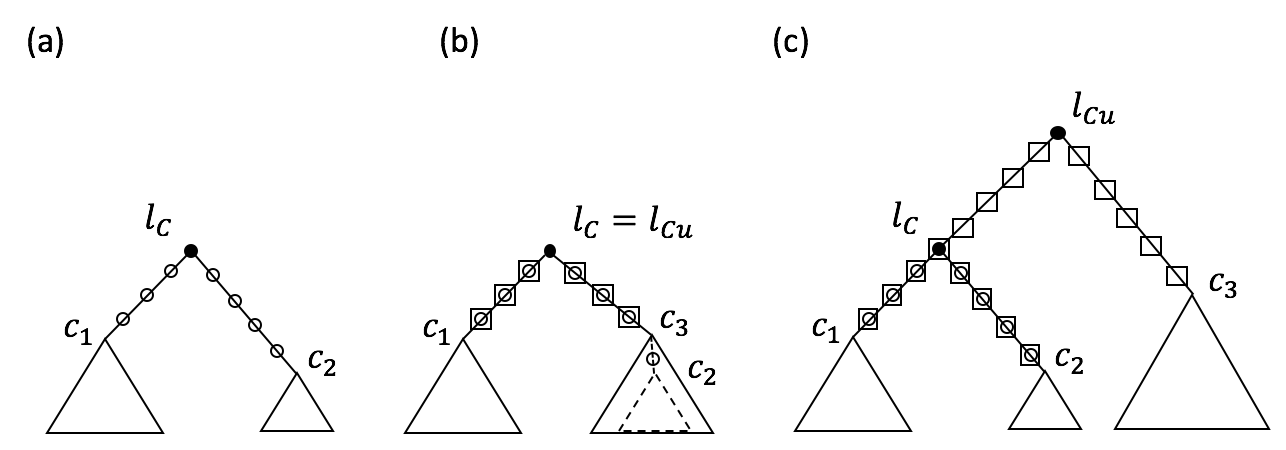
\includegraphics[scale=0.6]{incompatibilityrecursive}
        \centering
        \caption[Recursively defining incompatibility]{Illustration of a recursive definition of incompatibility. Let $minCover^{T}(C) = \{c_1, c_2\}$ and circled nodes be in $incompatible^{T}(C)$, as in (a). For some node $u \in V(T)$, let $Cu = C \cup \leafset^{T}(u)$ and the nodes $l_C$ and $l_{Cu}$ be $lca^{T}(C)$ and $lca^{T}(Cu)$ respectively. In (b), $minCover^{T}(Cu) = \{c_1, c_3\}$, and $l_C = l_{Cu}$, while in (c), $minCover^{T}(Cu) = \{c_1, c_2, c_3\}$ and $l_C \neq l_{Cu}$. In both (b) and (c), nodes belonging to $incompatible^{T}(Cu)$ are marked with squares and $coverer^{T, Cu}(u) = c_3$.}
        \label{fig:incompatibilityrecursive}
    \end{figure}

    We use observations from Figure~\ref{fig:incompatibilityrecursive} to gain intuition that helps us develop this operation. Let $minCover^{T}(C) = \{c_1, c_2\}$ and circled nodes belong to $incompatible^{T}(C)$, as shown in Figure~\ref{fig:incompatibilityrecursive}(a). For some node $u \in V(T)$, let $Cu = C \cup \leafset^{T}(u)$ and the nodes $l_C$ and $l_{Cu}$ be $lca^{T}(C)$ and $lca^{T}(Cu)$ respectively. Then Figure~\ref{fig:incompatibilityrecursive}(b) gives a case where $minCover^{T}(Cu) = \{c_1, c_3\}$. Here, $l_C = l_{Cu}$. Nodes in $incompatible^{T}(Cu)$ are marked with squares. Observe that the nodes in $path^{T}(c_2, c_3] = path^{T}(c_2, coverer^{T, Cu}(u)]$ belonged to $incompatible^{T}(C)$ but do not belong to $incompatible^{T}(Cu)$. The case where $minCover^{T}(Cu) = \{c_1, c_2, c_3\}$ and $l_C \neq l_{Cu}$ is shown in Figure~\ref{fig:incompatibilityrecursive}(c). In this case, we have to add the nodes in $path^{T}(c_3, l_{Cu}) = path^{T}(coverer^{T, Cu}(u), l_{Cu})$ and $path^{T}(l_C, l_{Cu})$ to $incompatible^{T}(C)$ to get $incompatible^{T}(Cu)$. We need to be a little careful with adding $l_C$ to $incompatible^{T}(C)$ though. Firstly, if $\leafset^{T}(l_C) = C$, then $\leafset^{T}(l_C) \subseteq Cu$, so it should not be added. However, if $\leafset^{T}(l_C) \neq C$ (and $l_C \neq l_{Cu}$) then it should be added. These observations are encapsulated in the following Lemma.
    \newline

    \begin{incompatibilityrecursive}
        \label{lem:incompatibilityrecursive}

        Given a tree $T$ leaf-labelled by $L$, a cluster $C \subseteq L$ and a node $u \in V(T)$ such that $\leafset^{T}(u) \cap C = \emptyset$, let $I = incompatible^{T}(C)$, $Cu = C \cup \leafset^{T}(u)$, $v = coverer^{T, Cu}(u)$, $l_C = lca^{T}(C)$ and $l_{Cu} = lca^{T}(Cu)$. Then $incompatible^{T}(Cu)$ can be defined as follows
        \begin{align*}
            incompatible^{T}(Cu) = &(I - path^{T}(u, v]) \cup path^{T}(v, l_{Cu}) \cup path^{T}(l_C, l_{Cu})\\
            &\cup
            \begin{cases}
                \{l_C\} & \leafset^{T}(l_C) \neq C \text{ and } l_C \neq l_{Cu}\\
                \emptyset & otherwise
            \end{cases}
        \end{align*}

        \begin{proof}
            By Lemma~\ref{lem:mincoverrecursive}, $minCover^{T}(Cu) - minCover^{T}(C) = \{v\}$ and $minCover(C) - minCover^{T}(Cu) \subseteq V(T[v])$. We represent the RHS of the equation in the Lemma by $X$.

            $\longrightarrow$. Take any node $w \in X$.

            Take the case where $w \in I - path^{T}(u, v]$. Since $w \in I$, there is some $c \in minCover^{T}(C)$ such that $w \in path^{T}(c, l_{C})$, by Lemma~\ref{lem:incompatibilitymincover}. If $c \not\in V(T[v])$, then $c \in minCover^{T}(Cu)$ and so $w \in incompatible^{T}(Cu)$. Otherwise, $c \in V(T[v])$. If $w$ is a proper ancestor of $v$, then $w \in incompatible^{T}(Cu)$. Otherwise, $w \in V(T[v])$. Since $w \in I - path^{T}(u, v]$, $w \not\in path^{T}(u, v]$, so $w$ is not an ancestor of $u$. Since $w \in incompatible^{T}(C)$, there is some leaf $x \in \leafset^{T}(w)$ such that $x \not\in C$. But also $x \not\in \leafset^{T}(u)$. Then $v \not\in minCover^{T}(Cu)$ because $x \in \leafset^{T}(v)$, which gives a contradiction, hence $w \not\in V(T[v])$.

            Otherwise, if $w \in path^{T}(v, l_{Cu})$, then $w \in incompatible^{T}(Cu)$ by Lemma~\ref{lem:incompatibilitymincover}.

            Otherwise, suppose $w \in path^{T}(l_C, l_{Cu})$. Then $C \subset \leafset^{T}(w)$. Also, $v$ is not a descendant of $w$, otherwise $w = l_{Cu}$. So $Cu - \leafset^{T}(w) \neq \emptyset$. Since $C \subset \leafset^{T}(w)$, there is some leaf $x \in \leafset^{T}(w)$ such that $x \not\in C$. Also, $x \not\in \leafset^{T}(u)$ since $v$ is not a descendant of $w$, so $x \not\in Cu$. Finally, $\leafset^{T}(w) \cap Cu \neq \emptyset$ because $C \subset \leafset^{T}(w)$ and $C \subset Cu$, thus $w \in incompatible^{T}(Cu)$.

            If none of the above are true, $w = l_C$ and $\leafset^{T}(l_C) \neq C$ and $l_C \neq l_{Cu}$. Clearly $\leafset^{T}(l_C) \cap Cu \neq \emptyset$. Since $\leafset^{T}(l_C) \neq C$, there is some leaf $x \in \leafset^{T}(l_C)$ such that $x \not\in C$. But also $x \not\in \leafset^{T}(u)$, other $l_C = l_{Cu}$. Thus $x \not\in Cu$, so $\leafset^{T}(l_C) \not\subseteq Cu$. Finally, $Cu \not\subseteq \leafset^{T}(l_C)$, since $l_C \neq l_{Cu}$. Thus $w \in incompatible^{T}(Cu)$.

            $\longrightarrow$. Take any node $w \in incompatible^{T}(Cu)$.

            By Lemma~\ref{lem:incompatibilitymincover}, there is some $c \in minCover^{T}(Cu)$ such that $w \in path^{T}(c, l_{Cu})$. If $c = v$, then $w \in X$. Otherwise, $c \in minCover^{T}(C)$ since $minCover^{T}(Cu) - minCover^{T}(C) = \{v\}$. If $w$ is a proper descendant of $l_C$, then $w \in I - path^{T}(u, v]$ by Lemma~\ref{lem:incompatibilitymincover}. If $w = l_C$, then $\leafset^{T}(l_C) \neq C$, otherwise $\leafset^{T}(l_C) \compatible Cu$. Also, $l_C \neq l_{Cu}$, since $l_{Cu} \not\in incompatible^{T}(Cu)$, so $w \in X$. Finally, if $w$ is a proper ancestor of $l_C$, then $w \in path^{T}(l_C, l_{Cu})$, so $w \in X$.
        \end{proof}
    \end{incompatibilityrecursive}

    Thus we define the operation $updateIncompatible^{T}(I, u, v, l_C, l_{Cu})$ which returns\\ $incompatible^{T}(Cu)$. The actual implementation of this operation is detailed in Subsection~\ref{subsec:updateincompatible}. We now make a claim about the running time of the $updateIncompatible$ operation, which is proved later.
    \newline

    \begin{updateincompatibleruntime}
        \label{lem:updateincompatibleruntime}

        Given a tree $T$ leaf-labelled by $L$, a cluster $C \subseteq L$ and a node $u \in V(T)$ such that $\leafset^{T}(u) \cap C = \emptyset$, let $I = incompatible^{T}(C)$, $Cu = C \cup \leafset^{T}(u)$, $l_C = lca^{T}(C)$, $l_{Cu} = lca^{T}(Cu)$ and $v = coverer^{T, Cu}(u)$. Let $removed$ be the set of nodes deleted from $I$ when calling $updateIncompatible^{T}(I, u, v, l_C, l_{Cu})$ and $added$ be the set of nodes inserted into $I$. Then the operation can be performed in $O(|added| + |removed|\,\times\,log\,n + 1)$ time, where $n = |\leafset^{T}|$.

        \begin{proof}
            Proved in Subsection~\ref{subsec:updateincompatible}.
        \end{proof}
    \end{updateincompatibleruntime}

    Note that the $log\,n$ factor comes about due to the data structure used to store $I$; this is explained in detail later.

    \subsection{Weighted Restricted Trees}
    \label{subsec:restrictedweighted}

    Recall the concept of restricted trees introduced in Subsection~\ref{subsec:restrictedtree} - given a tree $T$ leaf-labelled by $L$ and a cluster $C \subseteq L$, $V(T|C) = \{lca^T(u, v) : u, v \in C\}$ which obeys $lca^T(C') = lca^{T|C}(C')$ for all clusters $C' \subseteq C$. Observe that certain nodes are deleted from $T$ when forming $T|C$; this leads to losing information about the weights of these nodes. Hence, we extend the concept of restricted trees to the case where the tree is weighted, following the definition given in \cite{jansson2018algorithms}.

    Given a tree $T$ leaf-labelled by $L$, a cluster $C \subseteq L$ and for each node $u \in V(T)$, the value $\weight(u)$, we define the tree $T||C$, read as ``weighted $T$ restricted to $C$''. First, the tree $T|C$ is constructed and let the weight of each node in this tree be the same as its weight in $T$. Now for each non-root node $u \in V(T|C)$, let $v = parent^{T|C}(u)$. Then if $path^{T}(u, v) \neq \emptyset$ we create a dummy node $z$ in $T|C$ and set $parent(u) = z$ and $parent(z) = v$. Also, $\weight(z)$ is set as $max_{w \in path^{T}(u, v)} \weight(w)$. Intuitively, if $path^{T}(u, v) \neq \emptyset$, then the nodes in this path have been deleted from $T$ to form $T|C$. As we wish to retain some information about their weights, we insert the dummy node $z$ into $T||C$ to represent this path and hold the largest weight along it. Figure~\ref{fig:dummynodes} demonstrates this procedure.

    \begin{figure}[ht]
        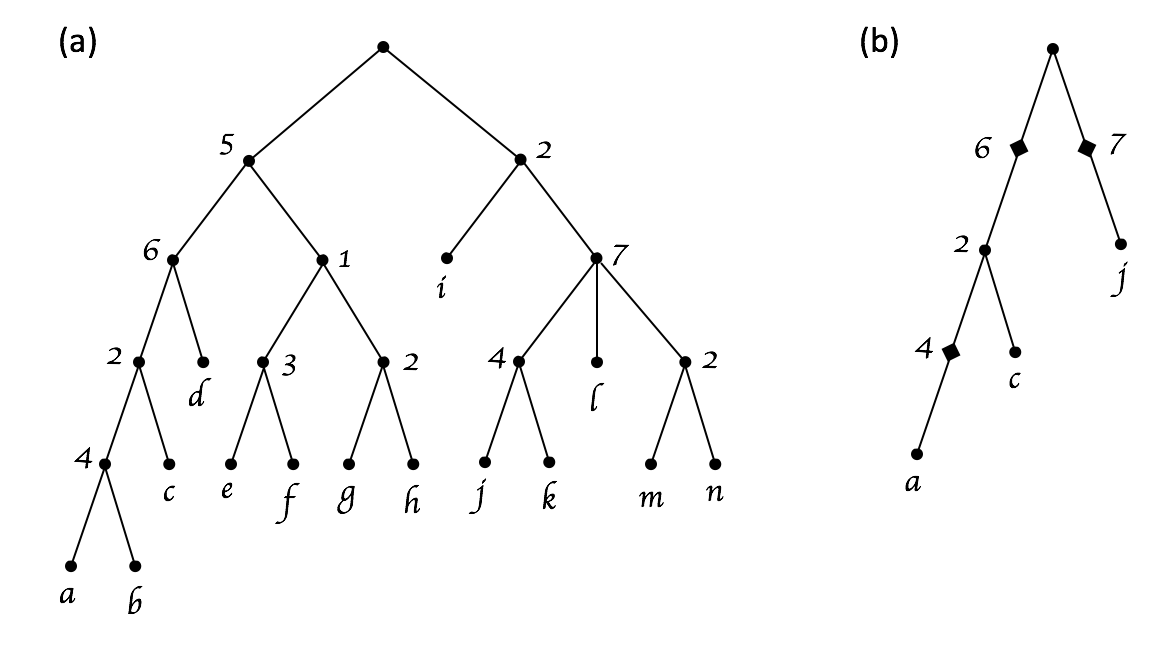
\includegraphics[scale=0.5]{dummynodes}
        \centering
        \caption[Constructing the tree $T||C$]{Part (a) shows a tree $T$ where all internal nodes are labelled with their weights. Part (b) shows the tree $T||C$, where $C = \{a, c, j\}$. Again, internal nodes are labelled with their weights. Nodes represented by diamonds in this figure are dummy nodes. Observe that the dummy node that is a parent of the leaf $j$ has weight $7$ since the nodes on the path from $j$ to the root of $T$ had weights $4, 7$ and $2$. The only pure nodes in this tree are the leaves.}
        \label{fig:dummynodes}
    \end{figure}

    Now, we observe some properties of $T||C$. First, define the pure nodes in $T$ with respect to $C$, denoted as $pure^{T}(C)$, to be the set $\{\leafset^{T}(u) \subseteq C : u \in V(T)\}$. Observe that $pure^{T}(C) = \bigcup_{c \in minCover^{T}(C)} V(T[c])$, i.e. the set of nodes that belong to the subtrees rooted at the minimum cover of $C$ in $T$. Notice that for any node $u \in pure^{T}(C)$, since $\leafset^{T}(u) \subseteq C$, $u \in V(T|C)$ and so $u \in V(T||C)$. Thus these subtrees are copied over without change to $T||C$. Now define the impure nodes in $T||C$, denoted as $impure^{T}(C)$, to be the set $V(T||C) - pure^{T}(C)$. Observe that all dummy nodes in $T||C$ belong to $impure^{T}(C)$. Now we prove a Lemma about the incompatibility of nodes in $T||C$.
    \newline

    \begin{impurenodesincompatible}
        \label{lem:impurenodesincompatible}

        Given a tree $T$ leaf-labelled by $L$, a cluster $C \subseteq L$ and for each node $u \in V(T)$, the value $\weight(u)$. Further, take any cluster $C' \subseteq C$ and any node $u \in impure^{T}(C)$, such that $u$ is a proper descendant of $lca^{T||C}(C')$. Then for any node $v \in V(T)$ that is represented by $u$, $\leafset^{T}(v) \not\compatible C'$.

        \begin{proof}
            Take the case where $u$ is a dummy node. Then let the nodes $w, w' \in V(T)$ be such that $u$ represents $path^{T}(w, w')$ and take any node $v \in path^{T}(w, w')$. Since $u$ is a proper descendant of $lca^{T||C}(C')$, $v$ is a proper descendant of $lca^{T}(C')$. Further, since $w$ is also a proper descendant of $lca^{T||C}(C')$ and $w \in V(T|C)$, $\leafset^{T}(w) \cap C' \neq \emptyset$. Also, if $\leafset^{T}(v) \subseteq C'$, then $v \in V(T|C)$, but that contradicts the construction of $T||C$. Thus $\leafset^{T}(v) \not\compatible C'$.

            Take the case where $u$ is not a dummy node. Then $u$ only represents itself. Further, $u \in V(T)$ and $u$ is a proper descendant of $lca^{T}(C')$. Since it is also true that $u \in V(T|C)$, $\leafset^{T}(u) \cap C' \neq \emptyset$. Finally, if $\leafset^{T}(u) \subseteq C'$ then $u \in pure^{T}(C)$, but that contradicts the underlying assumption that $u \in impure^{T}(C)$. Thus $\leafset^{T}(u) \not\compatible C'$.
        \end{proof}
    \end{impurenodesincompatible}

    Recall that we need to make queries of the form $max_{w \in path^{T}(u, v)} \weight(w)$, where $u, v \in V(T)$, in order to construct a weighted restricted tree. Notice that we can answer this with a query of the form $rmqTree^{T}[parent(u), cFD(v)]$, which we denote by $rmqTree^{T}(u, v)$. We now show that to further restrict a weighted restricted tree, we can use RMQ and cFD structures constructed on the original tree.
    \newline

    \begin{restrictedrmq}
        \label{lem:restrictedrmq}

        Given a tree $T$ leaf-labelled by $L$, clusters $C \subseteq L$ and $C' \subseteq C$, for each node $u \in V(T)$, the value $\weight(u)$ and RMQ and cFD structures on $T$. The tree $(T||C)||C'$ can be constructed from the tree $T||C$ using $rmqTree$ queries on $T$.

        \begin{proof}
            The key insight here is that no dummy node in $T||C$ belongs to $(T||C)||C'$. The reason for this is that any dummy node has only one child, and so can never be the $lca$ of any cluster. Thus, we only need to make $rmqTree^{T||C}(u, v)$ queries, where $u, v \in V(T||C)$ and $u, v$ are not dummy nodes. But since these are not dummy nodes, $u, v \in V(T)$. Since the construction of $T||C$ guarantees that $rmqTree^{T||C}(u, v) = rmqTree^{T}(u, v)$, we can use the RMQ and cFD structures on $T$ to answer these queries.
        \end{proof}
    \end{restrictedrmq}

    \subsection{The \texttt{Filter\_Clusters} algorithm}
    \label{subsec:filterclusters}

    With these operations in hand, we now develop the solution for \texttt{Filter\_Clusters}. Recall that this method takes trees $\TA$ and $\TB$ as input. First, for any node $u \in V(\TA)$, define $incompatible^{\TB}(u)$ to be $incompatible^{\TB}(\leafset^{\TA}(u))$. As discussed earlier, the idea is to find $incompatible^{\TB}(u)$ for each node $u \in V(\TA)$.

    We present a procedure similar to the algorithm \texttt{Filter\_Clusters} in \cite{jansson2018algorithms}. This procedure takes trees $\TA$ and $\TB$ as input, where $\leafset^{\TA} = \leafset^{\TB} = L$. It returns a forest $\mathcal{F}$ such that the clusters in this forest are the ones from $\TA$ whose weight is more than the heaviest incompatible cluster in $\TB$; i.e. $\bigcup_{T \in \mathcal{F}} \mathcal{C}(T) = \{C : C \in \mathcal{C}(\TA) \text{ and } \weight(C) > max(\{\weight(C_1) : C_1 \in \mathcal{C}(\TB) \text{ and } C_1 \not\compatible C\})\}$. Note that since the root of the original $\TA$ is a trivial cluster, it is compatible with all other clusters, so it will never be deleted. Thus, the outermost recursive call will yield only a single tree. Our procedure also returns the set $minCover^{\TB}(\leafset^{\TA})$. Note that we call this also call this modified procedure \texttt{Filter\_Clusters} for ease.

    Algorithm~\ref{alg:filterclusters} gives the algorithm \texttt{Filter\_Clusters}. Step~\ref{step:centroidpath} decomposes $\TA$ into a \textit{centroid path} $\langle p_{\gamma}, p_{\gamma - 1}, \dots, p_1 \rangle$, where $p_{\gamma}$ is the root of $\TA$, and a set of \textit{side trees} (similarly to \cite{jansson2018algorithms}). Observe that for any side tree $\tau \in \sigma(\TA)$, $|\leafset^\tau| \leq n/2$ and that $\{\leafset^{\tau} : \tau \in \sigma(\TA)\}$ forms a partition of $L\, \backslash\, {p_1}$. We further note that for any internal node $p_i \in \pi(\TA)$, $\leafset^{\TA}(p_{i - 1}) \subset \leafset^{\TA}(p_i)$, i.e. the cluster associated with $p_{i-1}$ is a proper subset of $p_i$. This then leads to the intuition behind the procedure \texttt{Filter\_Clusters} - recursively run the algorithm on the side trees, and then iterate over the centroid path from leaf to root, finding $incompatible^{\TB}(p_i)$ for each $p_i \in \pi(\TA)$.

    More specifically, Step~\ref{step:recursivecall} first recursively calls, for each $\tau \in \sigma(\TA)$, \texttt{Filter\_Clusters}$(\tau, \TB||\leafset^{\tau})$. From these calls, Step~\ref{step:obtainsidecover} obtains the set $\bigcup_{\tau \in \sigma(p_i)} minCover^{\TB}(\leafset^{\tau})$ for each $p_i \in \pi(\TA)$. This set is denoted by $sideCover^{\TB}(p_i)$. Note that building the trees $\TB||\leafset^{\tau}$ requires RMQ and cFD data structures on $\TB$ to allow $rmqTree$ queries. To facilitate this, we contruct these before the outermost call to \texttt{Filter\_Clusters}.

    Before iterating over the centroid path, we do some setup for $p_1$ in Steps~\ref{step:p1cover} and~\ref{step:p1incompatible}, where the set of nodes incompatible with the leaf $p_1$ is empty and the minimum cover is just the leaf in $\TB$ labelled by $p_1$. Then for-loop in Step~\ref{step:outerfor} iterates over the remaining nodes in the centroid path from bottom to top. The sets $minCover^{\TB}(\leafset^{\TA}(p_{i-1}))$ and $incompatible^{\TB}(\leafset^{\TA}(p_{i-1}))$ are obtained from the previous iteration of the loop. Then for each node $c \in sideCover^{\TB}(p_i)$, we find its coverer and then iteratively add it to the minimum cover of $p_{i-1}$ in Steps~\ref{step:findcoverer} and~\ref{step:addtocover}. Then we update the set of incompatible nodes in Step~\ref{step:updateincompatible}.

    The maximum weight of any node in the incompatible set is obtained and compared against the weight of $p_i$ in Step~\ref{step:maximumweight}. If $p_i$ is not to be deleted, then we attach the trees in the forest obtained from the previous iteration and the trees in the forests obtained from the side trees to $p_i$. Otherwise, we simply take the union of these forests to create a larger one.

    \begin{algorithm}[!ht]
        \caption{Filter\_Clusters}
        \label{alg:filterclusters}

        \begin{algorithmic}[1]
            \Input Trees $\TA$ and $\TB$ with $\leafset^{\TA} = \leafset^{\TB} = L$ where every cluster has a known $weight$.

            \Output The forest $\mathcal{F}$ such that $\bigcup_{T' \in \mathcal{F}} \mathcal{C}(T') = \{C : C \in \mathcal{C}(\TA) \text{ and } \weight(C) > max(\{\weight(C_1) : C_1 \in \mathcal{C}(\TB) \text{ and } C_1 \not\compatible C\})\}$ and the set of nodes $minCover^{\TB}(\leafset^{\TA})$.

            \State Compute a centroid path $\pi = \langle p_{\gamma}, p_{\gamma - 1}, \dots, p_1 \rangle$ of $\TA$, where $p_{\gamma}$ is the root of $\TA$ and $p_1$ is a leaf.
            \label{step:centroidpath}

            \State Preprocess $\TB$ for lca queries.
            \label{step:preprocesslca}

            \State \algorithmicforall\ $p_i \in \pi(\TA)$, $sideCover^{\TB}(p_i) := \emptyset$, $\mathcal{F}_{p_i} := \emptyset$

            \ForAll{$\tau \in \sigma(\TA)$}
                \State $\mathcal{F}', sideCover' :=$ \texttt{Filter\_Clusters}$(\tau, \TB||\leafset^{\tau})$
                \label{step:recursivecall}

                \State $sideCover^{\TB}(p_i) := sideCover^{\TB}(p_i) \cup sideCover'$ and $\mathcal{F}_{p_i} := \mathcal{F}_{p_i} \cup \mathcal{F}'$, where $\tau$ is associated with \hspace*{\algorithmicindent}$p_i \in \pi(\TA)$
                \label{step:obtainsidecover}
            \EndFor

            \State $l :=$ leaf in $\TB$ labelled by $p_1$

            \State $cover := \{l\}$
            \label{step:p1cover}

            \State $incompatible :=$ empty Brodal queue
            \label{step:p1incompatible}

            \State $\mathcal{F} := \emptyset$

            \For{$i := 2$ \textbf{to} $\gamma$}
                \label{step:outerfor}
                \ForAll{$u \in sideCover^{\TB}(p_i)$}
                    \label{step:innerfor}

                    \State $v :=$ \texttt{Find\_Coverer}$(cover, u)$
                    \label{step:findcoverer}

                    \State $cover := cover \cup \{v\} - \bigcup_{w \in path^{T}(u, v]} children(w)$
                    \label{step:addtocover}

                    \State $l' := lca^{\TB}(l, u)$

                    \State $incompatible :=$ \texttt{Update\_Incompatible}$(incompatible, u, v, l, l')$
                    \label{step:updateincompatible}

                    \State $l := l'$
                \EndFor

                \If{$\weight(p_i) \leq$ maximum weight of a node in $incompatible$}
                    \label{step:maximumweight}
                    \State $\mathcal{F} = \{\text{A tree where each tree in } \mathcal{F} \cup \mathcal{F}_{p_i} \text{ is attached to a common root}\}$.
                \Else
                    \State $\mathcal{F} = \mathcal{F} \cup \mathcal{F}_{p_i}$
                \EndIf
            \EndFor

            \State \Return $\mathcal{F}, cover$
        \end{algorithmic}
    \end{algorithm}

    The key to analysing the runtime of \texttt{Filter\_Clusters} is the insight that no node is deleted from $incompatible$ twice. Intuitively, this is because nodes are removed from $incompatible$ when their leafsets become subsets of the cluster under consideration. Then this node, or an ancestor of this node, will become part of the cover, and eventually the side cover when the algorithm returns. Then this node can never be incompatible with any cluster under consideration again. Thus, over \textit{all} calls to \texttt{Filter\_Clusters}, the total number of deletions is $\leq |V(\TB)|$.

    We prove this claim in three parts. First, we show that the set of nodes deleted from $incompatible$ in separate recursive calls are disjoint.
    \newline

    \begin{numremovednodesrecursive}
        \label{lem:numremovednodesrecursive}

        Given trees $\TA$ and $\TB$, where $\leafset^{\TA} = \leafset^{\TB} = L$, and some node $p_i \in \pi(\TA)$. Then for any node $u \in V(\TB)$ such that $u$ is deleted from $incompatible$ when processing $p_i$, $u$ must be a descendant of some node $c_{p} \in minCover^{\TB}(\leafset^{\TA}(p_i))$ and a proper ancestor of some node $c_s \in sideCover^{\TB}(p_i)$.

        \begin{proof}
            $u$ is deleted from $incompatible$ if it is incompatible with some subset of $\leafset^{\TA}(p_i)$ and compatible with $\leafset^{\TA}(p_i)$. This only happens when $\leafset^{\TB}(u) \subseteq \leafset^{\TA}(p_i)$. But then there must be some ancestor $c_p$ of $u$ such that $c_p \in minCover^{\TB}(\leafset^{\TA}(p_i))$.

            By Lemma~\ref{lem:incompatibilityrecursive}, when we update the set of incompatible nodes with some node $c \in V(\TB)$, we only delete the nodes in $path^{\TB}(c, c']$, where $c'$ is the coverer of $c$. Thus we can only delete nodes that are proper ancestors of $c$. Since Step~\ref{step:updateincompatible} updates the incompatible set with nodes from $sideCover^{\TB}(p_i)$, we can only delete nodes that are proper ancestors of nodes in the side cover.
        \end{proof}
    \end{numremovednodesrecursive}

    Recalling that the side cover of $p_i$ is composed of the minimum covers of the side trees associated with $p_i$, it is clear that the set of nodes deleted in recursive calls is disjoint. We now show that in any single call to \texttt{Filter\_Clusters}, the sets of nodes deleted from $incompatible$ during an $updateIncompatible$ operation are also disjoint.
    \newline

    \begin{numremovednodescentroid}
        \label{lem:numremovednodescentroid}

        Given trees $\TA$ and $\TB$, where $\leafset^{\TA} = \leafset^{\TB} = L$. Then during the call \texttt{Filter\_Clusters}$(\TA, \TB)$, no node is deleted from $incompatible$ twice.

        \begin{proof}
            Take any node $u \in V(\TB)$ such that $u$ is first deleted from $incompatible$ during the processing of some $p_i \in \pi(\TA)$. By the same argument as in Lemma~\ref{lem:numremovednodesrecursive}, $\leafset^{\TB}(u) \subseteq \leafset^{\TA}(p_i)$. Then $\leafset^{\TB}(u) \compatible p_j$ for all $j \geq i$, as the nodes on the centroid path have nested leafsets. Thus $u$ will not be added to $incompatible$ again and so will not be deleted again.
        \end{proof}
    \end{numremovednodescentroid}

    We have shown above that no node is deleted twice from $incompatible$. However, recall that we create some dummy nodes, hence it remains to be shown that these nodes are never deleted from $incompatible$.
    \newline

    \begin{numremovednodesdummy}
        \label{lem:numremovednodesdummy}

        No dummy node is deleted from $incompatible$.

        \begin{proof}
            When a dummy node is added to $incompatible$, it must be a proper descendant of the $lca$ of the respective cluster by Lemma~\ref{lem:incompatibility}. Since we are considering nested clusters, it must also be a proper descendant of the $lca$ of all subsequent clusters. Then by Lemma~\ref{lem:impurenodesincompatible}, the dummy node is incompatible with all such subsequent clusters, so it will not be deleted from $incompatible$.
        \end{proof}
    \end{numremovednodesdummy}

    \medskip
    \begin{numremovednodes}
        \label{lem:numremovednodes}

        The total number of nodes deleted from $incompatible$ over all calls to\\ \texttt{Filter\_Clusters} is $\leq |V(\TB)|$.

        \begin{proof}
            Lemmas~\ref{lem:numremovednodesrecursive},~\ref{lem:numremovednodescentroid} and~\ref{lem:numremovednodesdummy} together show that any node in $\TB$ is only deleted once over all calls to \texttt{Filter\_Clusters}, and that these are the only nodes deleted. Thus total number of deletions $\leq |V(\TB)|$.
        \end{proof}
    \end{numremovednodes}

    Recall that the runtime of \texttt{Update\_Incompatible} depends both on the number of nodes removed and added. Thus, we also need to give an upper bound on the number of nodes added during calls to this function. This upper bound can be looser than the one for removed nodes, since insertions only cost us constant time. Hence, we only show that the number of additions is $O(|V(\TB)|)$ for a \textit{single} call to \texttt{Filter\_Clusters}, i.e. we only analyse over the centroid path, rather than the entirety of $\TA$.
    \newline

    \begin{numaddednodes}
        \label{lem:numaddednodes}

        Given trees $\TA$ and $\TB$, where $\leafset^{\TA} = \leafset^{\TB} = L$. Then during the call \texttt{Filter\_Clusters}$(\TA, \TB)$, no node is added to $incompatible$ twice.

        \begin{proof}
            Follows from the argument in Lemma~\ref{lem:numremovednodescentroid}.
        \end{proof}
    \end{numaddednodes}

    \medskip
    \begin{filterclustersruntime}
        \label{lem:filterclustersruntime}

        For some trees $\TA$ and $\TB$ where $\leafset^{\TA} = \leafset^{\TB} = L$ and $n = |L|$, the algorithm \texttt{Filter\_Clusters}$(\TA, \TB)$ runs in $O(n\,log\,n)$ time, if RMQ and cFD structures on $\TB$ are given.

        \begin{proof}
            The centroid path can be computed in Step~\ref{step:centroidpath} in $O(n)$ time.  The $lca$ data structure in Step~\ref{step:preprocesslca} can also be constructed in $O(n)$ time, by Lemma~\ref{lem:lca}. For Step~\ref{step:recursivecall}, since the side trees $\sigma(\TA)$ give a partition of $L$, the trees $\TB|\leafset^{\tau}$ for each $\tau \in \sigma(\TA)$ can be constructed in $O(n)$ time total using Lemma 5.2 of \cite{farach1995fast}. From these, $\TB||\leafset^{\tau}$ can be constructed in further $O(n)$ time since we can carry out $rmqTree$ queries in constant time, since we have RMQ and cFD structures on the original $\TB$ and by Lemmas~\ref{lem:rmqquery} and~\ref{lem:restrictedrmq}. Merging the $\mathcal{F}$ and $sideCover$ sets in Step~\ref{step:obtainsidecover} costs $O(1)$ time if we implement them as linked lists.

            We use the Brodal queue of \cite{brodal1995fast} to store incompatible nodes. This data structure allows $insert$ and $findMax$ operations in $O(1)$ time and $delete$ in $O(log\,m)$ time (where $m$ is the number of elements in the queue). Since the number of nodes in $\TB$ is $O(n)$, the number of elements in the queue is always $O(n)$ and so deletions cost $O(log\,n)$ time (this leads to the $log\,n$ factor seen in Lemma~\ref{lem:updateincompatibleruntime}).

            Since the total size of the leafsets of the side trees of $\TA$ is $n - 1$, the total size of the side covers is bounded by $n$. Then, the inner for-loop in Step~\ref{step:innerfor} is entered $\leq n$ times. Thus all constant time operations within this loop cost $O(n)$ time in total.

            In Step~\ref{step:findcoverer}, if the algorithm \texttt{Find\_Coverer} is called on some node $u \in V(\TB)$ and $v$ is its coverer, then the runtime of the algorithm depends on the size of the set $path^{\TB}(u, v]$. Observe that these nodes are then deleted from $incompatible$ in Step~\ref{step:updateincompatible}. By Lemma~\ref{lem:numremovednodescentroid}, the total number of nodes deleted from $incompatible$ during the function is $\leq |V(\TB)|$, so this function costs $O(|V(\TB)|)$ time in total.

            The nodes deleted from $cover$ in Step~\ref{step:addtocover} are children of the nodes deleted from $incompatible$. Again, since for any node, its parent is only deleted from $incompatible$ once, the node itself is only deleted from $cover$ once. These deletions are implemented in constant time using a linked list, hence Step~\ref{step:addtocover} costs $O(|V(\TB)|)$ time in total.

            We now analyse Step~\ref{step:updateincompatible}, where the set $incompatible$ is updated. By Lemma~\ref{lem:numaddednodes}, $\leq |V(\TB)|$ nodes are added in this step. Insertions into a Brodal queue take constant time, so additions take $O(|V(\TB)|)$ time. We analyse deletions from this set over \textit{all} calls to \texttt{Filter\_Clusters}. By Lemma~\ref{lem:numremovednodes}, the total number of deletions is $O(|V(\TB)|)$. Since the number of items in the queue never exceeds $|V(\TB)|$, a single deletion takes $log\,n$ time, and hence the deletions as a whole cost $O(n\,log\,n)$ time.

            Finally, getting the maximum weight from $incompatible$ in Step~\ref{step:maximumweight} costs constant due to the properties of Brodal queues. If the node is not to be deleted, then we attach all the forests in $\mathcal{F}$ to a common root. This costs $O(n)$ time in total since each node is attached to a root only once. Alternatively, inserting into $\mathcal{F}$ takes constant time if we implement it as a linked list of trees. Since any subtree of $\TA$ is inserted into $\mathcal{F}$ only once, this also costs $O(n)$ time.

            Thus for a single call to \texttt{Filter\_Clusters}, $T(n) = O(n) + \sum_{\tau \in \sigma(\TA)} T(|\leafset^{\tau}|)$. Since for any $\tau \in \sigma(\TA)$, $|\leafset^{\tau}| \leq n/2$, there are $log\,n$ recursion levels, and we get $T(n) = O(n\,log\,n)$. As the total cost over all calls due to removing nodes from $incompatible$ is also $O(n\,log\,n)$, the overall runtime of \texttt{Filter\_Clusters} is $O(n\,log\,n)$.
        \end{proof}
    \end{filterclustersruntime}

    \subsection{The $findCoverer$ operation}
    \label{subsec:findcoverer}

    The definition of $findCoverer$ in Lemma~\ref{lem:findcovererrecursive} gives Algorithm~\ref{alg:findcoverer}.

    \begin{algorithm}
        \caption{Find\_Coverer}
        \label{alg:findcoverer}

        \begin{algorithmic}[1]
            \Input For some tree $T$ leaf-labelled by $L$ and cluster $C \subseteq L$, takes in some node $u \in V(T)$, where $\leafset^{T}(u) \cap C = \emptyset$.

            \Output Let $Cu = C \cup \leafset^{T}(u)$. The algorithm outputs $coverer^{T, Cu}(u)$.

            \State $v := parent(u)$

            \If{$\leafset^{T}(v) \subseteq Cu$ and $v$ is pure}
                \State \Return \texttt{Find\_Coverer}$(v)$
            \Else
                \State \Return $u$
            \EndIf
        \end{algorithmic}
    \end{algorithm}

    Note that we need to make use of the concept of pure and impure nodes to make a query of the form $\leafset^{T}(v) \subseteq Cu$. This is because we wish to check incompatibility against the original $\TB$, but we instead have weighted restricted trees. Thus, we also check whether $v$ is pure. We now prove the claim in Lemma~\ref{lem:findcovererruntime}.

    \begin{proof}[Proof of Lemma~\ref{lem:findcovererruntime}]
        First, we need to give a way to implement the check for $\leafset^{T}(v) \subseteq Cu$. To do so, we give every node $w \in T$ a property $counter(w)$. $counter(w)$ initially stores $|\{\leafset^{T}(c) \subseteq C : c \in children(w)\}|$. We update this to reflect the addition of $\leafset^{T}(u)$ to $C$ by incrementing $counter(v)$, and then check whether $counter(v) = |children(v)|$, which is equivalent to determining if $\leafset^{T}(v) \subseteq Cu$. This allows us to make the check in $O(1)$ time.

        The recursive case of the algorithm is hit exactly $|path^{T}(u, v]|$ times, where $v = coverer^{T, Cu}(u)$. Each of these costs constant time. The base case is hit once, again costing constant time. Thus, the overall cost of the operation is $O(|path^{T}(u, v]| + 1)$.
    \end{proof}

    \subsection{The $updateIncompatible$ operation}
    \label{subsec:updateincompatible}

    We use the definition in Lemma~\ref{lem:incompatibilityrecursive} to construct Algorithm~\ref{alg:updateincompatible}.

    \begin{algorithm}
        \caption{Update\_Incompatible}
        \label{alg:updateincompatible}

        \begin{algorithmic}[1]
            \Input Given some tree $T$ leaf-labelled by $L$, cluster $C \subseteq L$ and some node $u \in V(T)$ where $\leafset^{T}(u) \cap C = \emptyset$. Let $Cu = C \cup \leafset^{T}(u)$. The algorithm takes in the set $I = incompatible^{T}(C)$ and the nodes $u$, $v = coverer^{T, Cu}(u)$, $l_C = lca^{T}(C)$ and $l_{Cu} = lca^{T}(Cu)$.

            \Output The algorithm outputs the set $incompatible^{T}(Cu)$.

            \State $I := (I - path^{T}(u, v]) \cup path^{T}(v, l_{Cu}) \cup path^{T}(l_C, l_{Cu})$

            \If{($\leafset^{T}(l_C) = C$ and $l_C$ is pure) or $l_C = l_{Cu}$}
                \State \Return $I$
            \Else
                \State \Return $I \cup \{l_C\}$
            \EndIf
        \end{algorithmic}
    \end{algorithm}

    Note that we again need to take the concept of pure and impure nodes into account when making the check for $\leafset^{T}(l_C) = C$. We now prove the claim in Lemma~\ref{lem:updateincompatibleruntime}.

    \begin{proof}[Proof of Lemma~\ref{lem:updateincompatibleruntime}]
        We implement the check for $\leafset^{T}(l_C) = C$ in constant time using the counter technique described in the proof of Lemma~\ref{lem:findcovererruntime}. This gives the constant term in the runtime expression.

        The incompatible nodes are stored in the Brodal queue of \cite{brodal1995fast}, described in the proof of Lemma~\ref{lem:filterclustersruntime}.

        Observe that when adding nodes along the paths, we can iterate upwards along these, adding the nodes while they are not already in $I$, and stopping as soon as we find one that already belongs to $I$. This check can also be implemented in constant time by giving each node a membership property. Since inserts into Brodal queues take $O(1)$ time, the total cost due to these additions is $O(|added|)$.

        We also delete $|removed|$ nodes from the queue. Deletions from a Brodal queue cost $O(log\,n)$ time, hence cost due to this is $O(|removed| \times log\,n)$.
    \end{proof}

    \section{Constructing the FDCT}
    \label{sec:freqdiffconstruction}

    \begin{freqdiffruntime}
        \label{theorem:freqdiffruntime}

        Given a set $\mathcal{S}$ of $k$ trees with identical leafsets of size $n$, the algorithm \texttt{Frequency\_Difference}$(\mathcal{S})$ runs in $O(kn\,log\,n)$ time.

        \begin{proof}
            By Corollary~\ref{cor:freqdiffruntimecomponents} and Lemmas~\ref{lem:weightingruntime} and~\ref{lem:filterclustersruntime}, \texttt{Frequency\_Difference} runs in $O(kn\,log\,n + k \cdot n\,log\,n) = O(kn\,log\,n)$ time.
        \end{proof}
    \end{freqdiffruntime}

    \section{Implementation}
    \label{sec:implementation}

    As noted in Subsection~\ref{subsec:previouswork}, there are two existing implementations that compute FDCTs - TNT \citep{goloboff2008tnt} and the FACT package \citep{jansson2016improved}. However, the results in \cite{jansson2018algorithms} demonstrated that their implementation outperforms TNT under all conditions, so we only make a comparison with this. Our implementation of the algorithm \texttt{Frequency\_Difference} reuses their code, with certain key optimisations, as laid out above. The code is written in C++ and utilises some libraries from the Boost package \citep{BoostLibrary}. The source can be found at \url{https://github.com/varung97/FACT2}. Note that there are some differences between the implementation and the algorithm described above, made for reasons of optimisation and readability. These differences are described in Subsection~\ref{subsec:implementationdetails}.

    The resulting implementation was compared with that from the FACT package by running them both on trees generated with various values of $k$ and $n$. This setup is described in Subsection~\ref{subsec:setup} and the results are presented in Subsection~\ref{subsec:results}.

    \subsection{Implementation Details}
    \label{subsec:implementationdetails}

    The differences between the described algorithm and our implementation are:

    \begin{enumerate}
        \item While the algorithm is fully deterministic, the implementation is not; we use hash sets instead of linked lists to store nodes in the minimum cover for ease.

        \item The algorithm \texttt{Find\_Coverer} is implemented iteratively instead of recursively for efficiency. Further, this procedure and the procedure \texttt{Update\_Incompatible} were moved inside the main body of the algorithm rather than separating them out into functions, again because this is faster.

        \item Rather than constructing the trees $\TB||\leafset^{\tau}$ and then inserting the nodes on certain paths into the Brodal queue, we simply obtain the maximum weight of nodes on the paths using $rmqTree$ queries and insert this maximum weight into the queue.
    \end{enumerate}

    \subsection{Experimental Setup}
    \label{subsec:setup}

    We generated input trees according to two different scenarios, exactly as in \cite{jansson2018algorithms}. The first scenario, ``Scenario 1'', is the situation where trees share a large percentage of clusters, which is largely realistic. On the other hand, the second scenario, ``Scenario 2'', generates completely independent trees, which represents the other end of the spectrum. In particular, the process for generating $k$ trees with leaf labels $\{1, 2, \dots, n\}$ under the two scenarios is:

    \begin{itemize}
        \item \textit{Scenario 1:} We generate a binary tree, with the given leaf labels, under the uniform model \citep{mckenzie2000distributions}. Then for each non-root internal node $u$ in this tree, we perform a $delete$ operation on $u$ with probability $0.2$. Then we make $k$ copies of this tree, and for each copy, we randomly select a non-root node $u$ and an internal node $v$ $n / 20$ times, remove the subtree rooted at $u$ and attach it to $v$.

        \item \textit {Scenario 2:} We generate $k$ binary trees, with the given leaf labels, each under the uniform model \citep{mckenzie2000distributions}. Then for each non-root internal node $u$ in each tree, we $delete$ $u$ with probability $0.2$.
    \end{itemize}

    Since we wished to see the effect of both $k$ and $n$ on these algorithms, we ran two experiments, one with $n$ fixed and one with $k$ fixed. Further, we measured the time taken by the weighting step and the remainder of the algorithm separately. Note that we use the running time of the second half of \texttt{Frequency\_Difference} as a stand-in for running time of \texttt{Filter\_Clusters} as it is hard to measure the latter independently, and since the implementations are identical except for \texttt{Filter\_Clusters}. For each value of $k$ and $n$, we generated 5 input examples and averaged the running time over these.

    We ran the experiments on a MacBook Pro laptop running macOS Sierra 10.12.6, equipped with 16GB RAM and a 2.2 GHz Intel Core i7 processor. The C++ compiler used was clang-802.0.42 and the version of the Boost libraries was 1.65.1. The time taken was measured using the inbuilt \texttt{clock()} function in C++.

    \subsection{Experimental Results}
    \label{subsec:results}

    \begin{table}[!ht]
        \captionsetup{font=footnotesize,justification=centering,margin=0cm}
        \fontsize{9}{11}\selectfont
        \begin{minipage}{0.49\textwidth}
            \centering
            \caption[Runtime of the Weighting step in Scenario 1, with $n = 1000$ and varying $k$]{Weighting time with $n = 1000$, varying $k$}
            \label{tab:weightk1}
            \begin{tabular}{c||ccccc}
                $k$ & $kn\,log\,n$ & $kn^2$ & $k^2n$\\
                \hline\hline
                50 & 0.34 & 0.04 & 0.04\\
                100 & 0.66 & 0.09 & 0.12\\
                200 & 1.32 & 0.17 & 0.46\\
                500 & 3.51 & 0.47 & 2.82\\
                1000 & 7.32 & 1.03 & 11.25\\
                2000 & 15.07 & 2.27 & 45.13\\
                3000 & 23.58 & 3.66 & 100.06\\
                4000 & 31.48 & 4.87 & 174.49\\
            \end{tabular}
            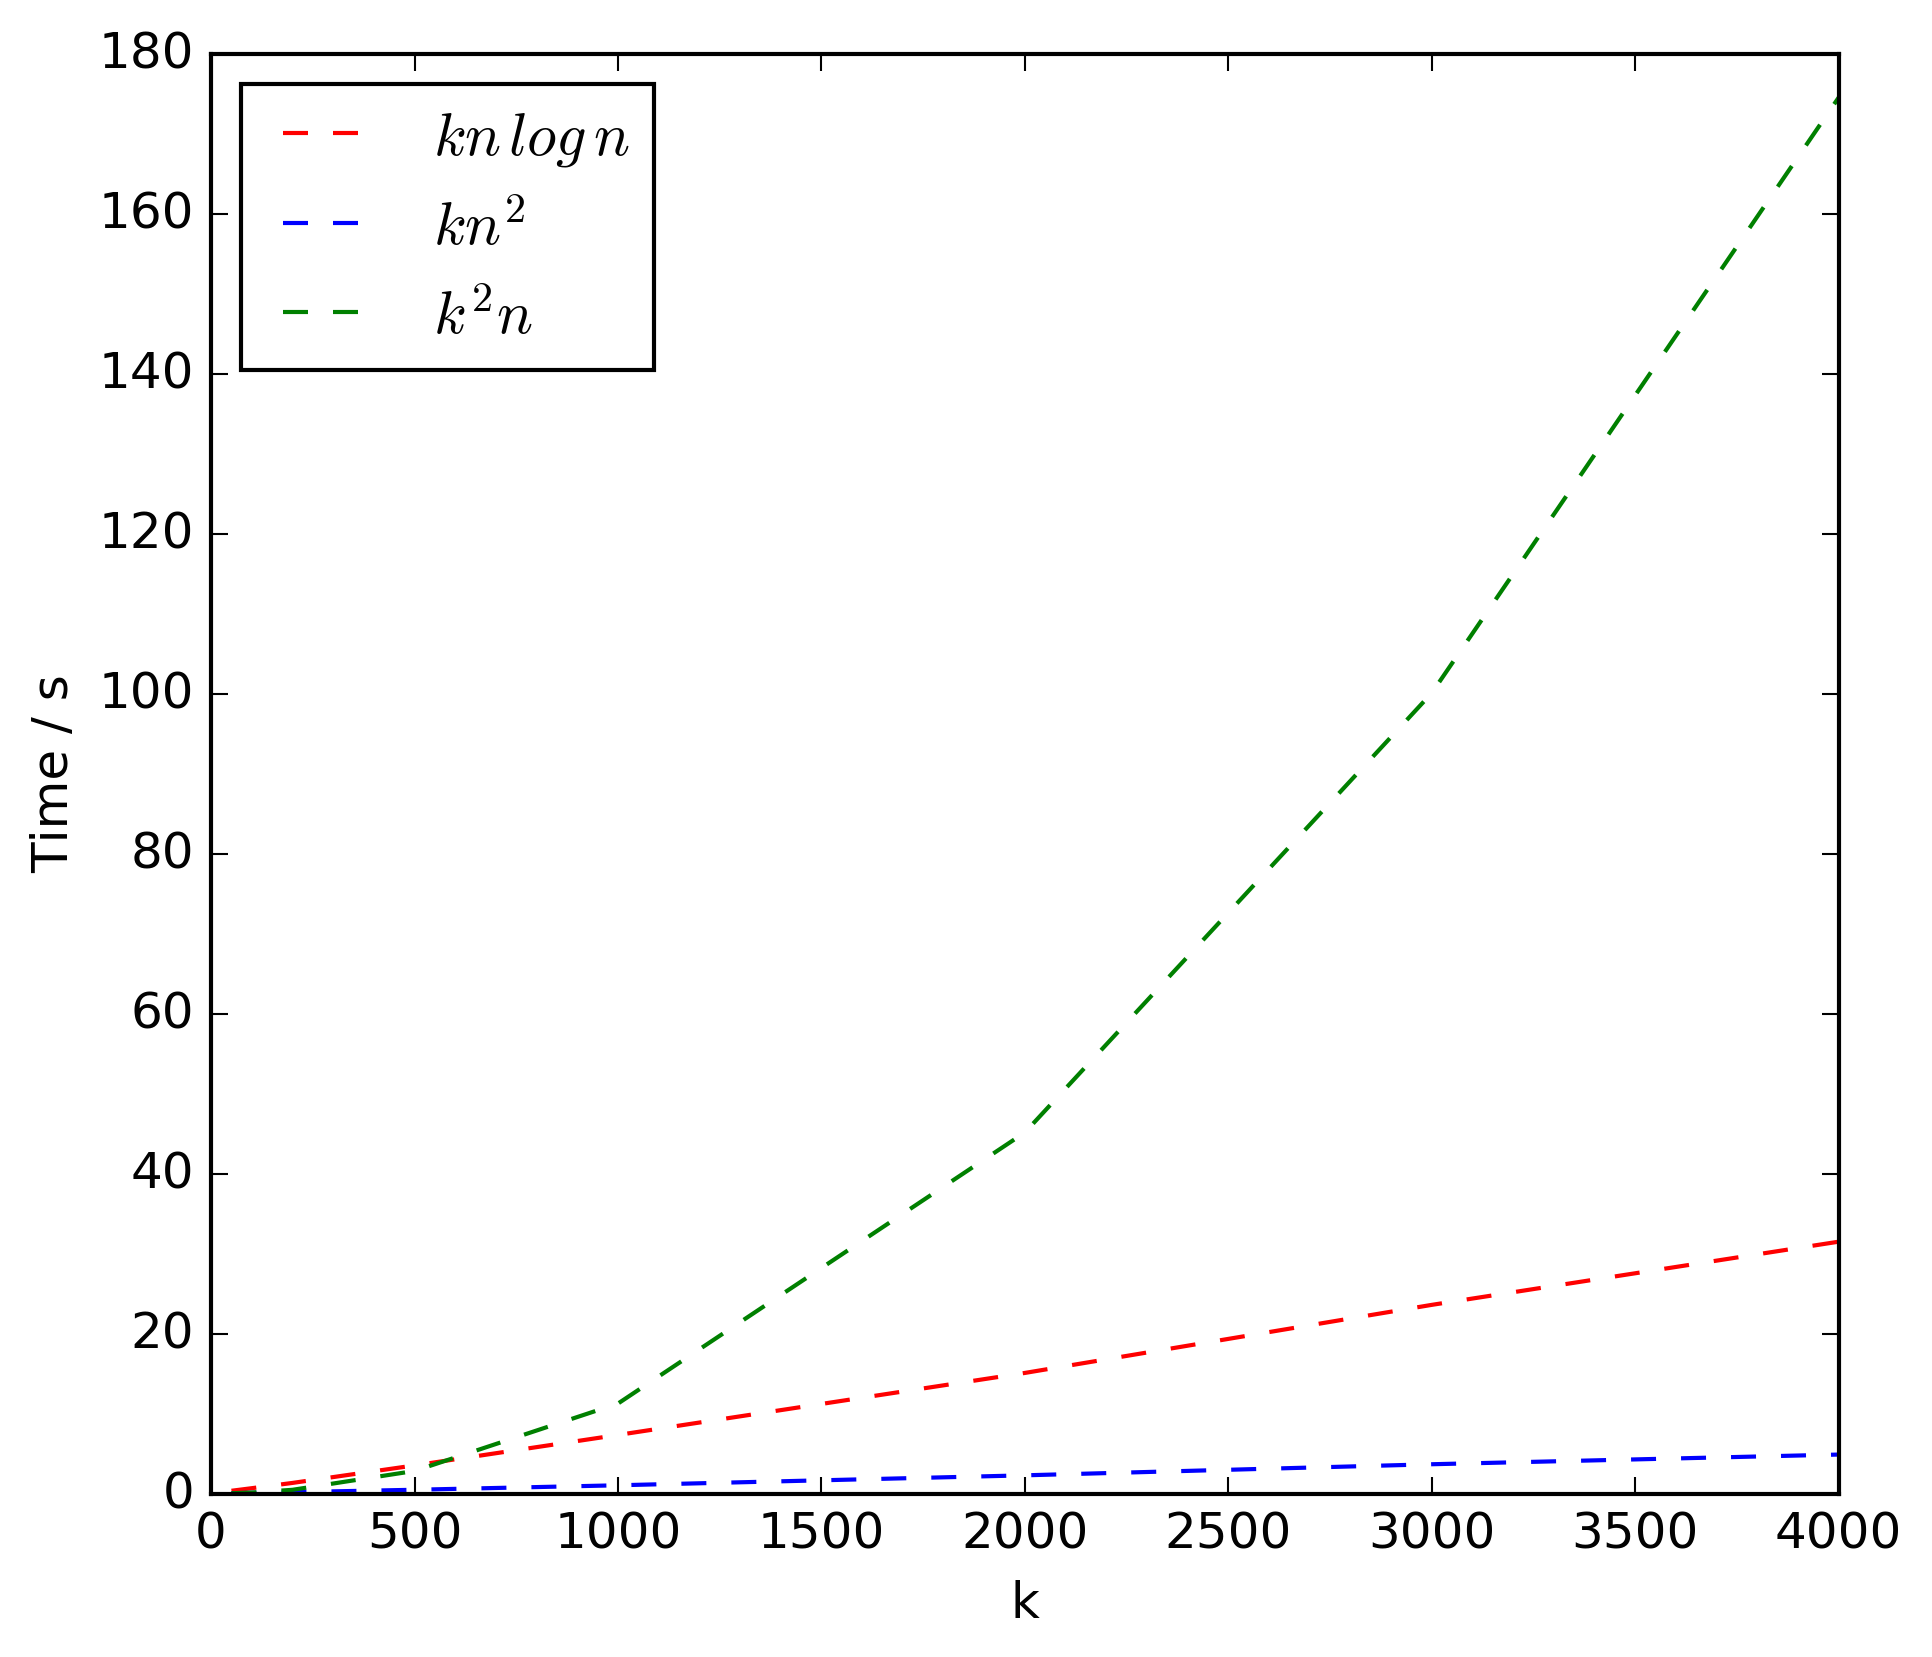
\includegraphics[scale=0.4]{varyingk1_weighting}
            \vspace{0.5cm}
        \end{minipage}\hfill
        \begin{minipage}{0.48\textwidth}
            \centering
            \caption[Runtime of \texttt{Filter\_Clusters} in Scenario 1, with $n = 1000$ and varying $k$]{\texttt{Filter\_Clusters} time with $n = 1000$, varying $k$}
            \label{tab:filterk1}
            \begin{tabular}{c||ccccc}
                $k$ & $n\,log\,n$ & $n\,log^2n$\\
                \hline\hline
                50 & 1.13 & 1.04\\
                100 & 2.31 & 2.52\\
                200 & 4.65 & 5.00\\
                500 & 11.89 & 13.90\\
                1000 & 24.84 & 27.39\\
                2000 & 52.71 & 62.18\\
                3000 & 81.01 & 84.99\\
                4000 & 108.53 & 116.16\\
            \end{tabular}
            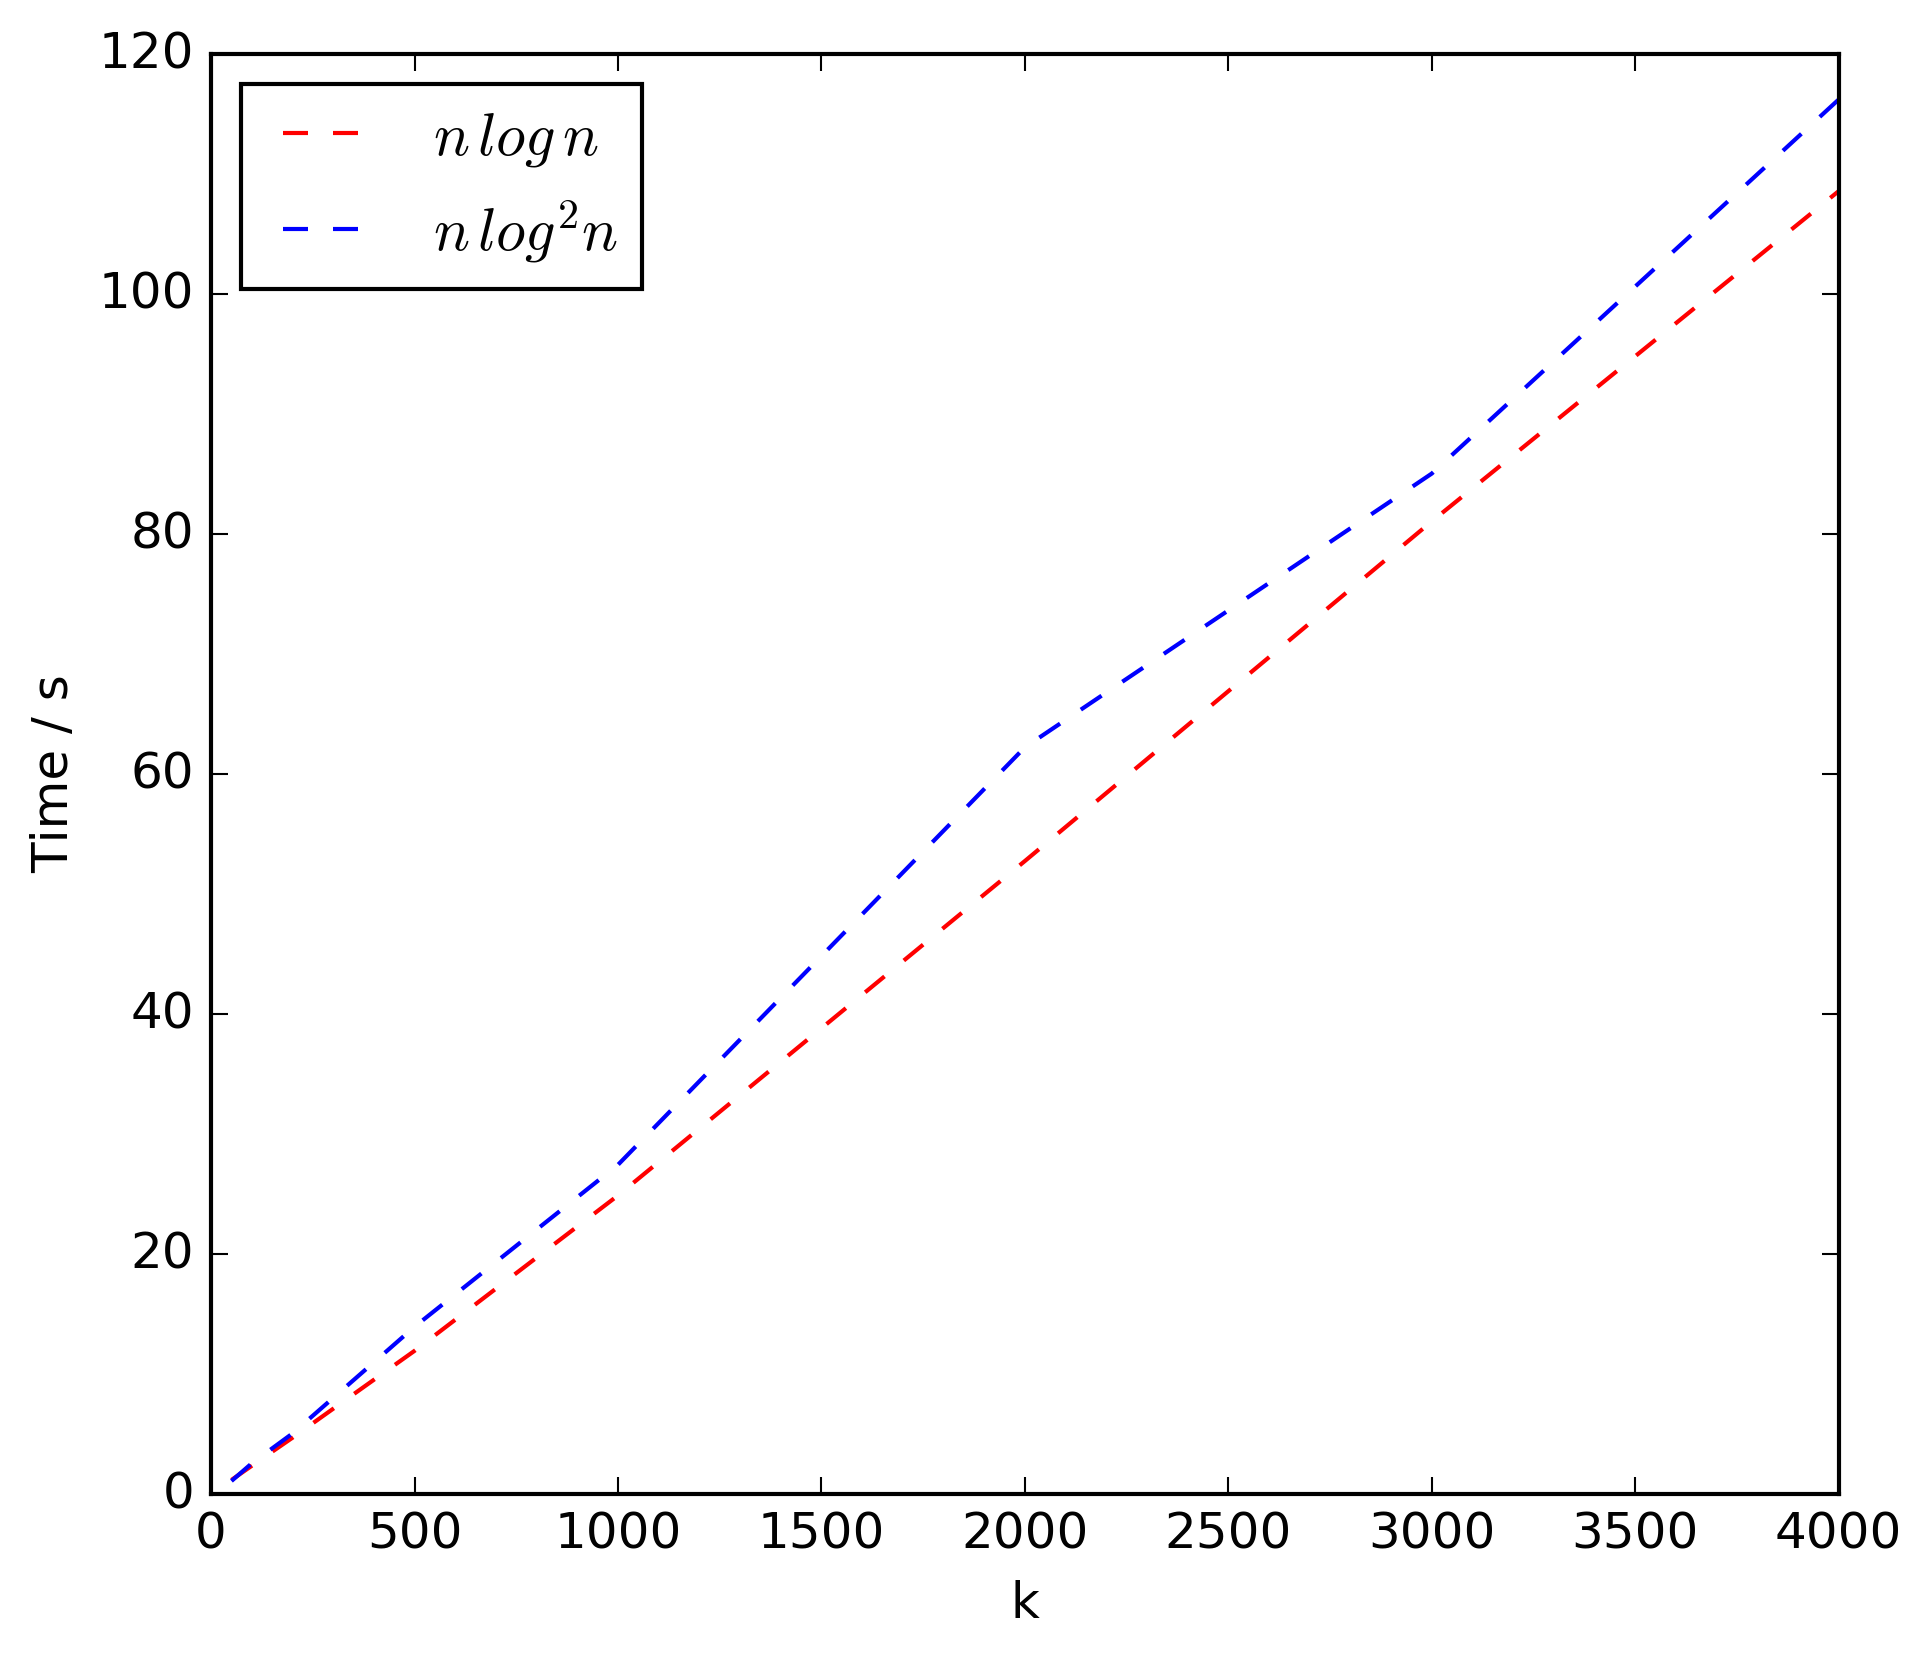
\includegraphics[scale=0.4]{varyingk1_filter}
            \vspace{0.5cm}
        \end{minipage}
        \begin{minipage}{0.48\textwidth}
            \centering
            \caption[Runtime of the Weighting step in Scenario 1, with $k = 100$ and varying $n$]{Weighting time with $k = 100$, varying $n$}
            \label{tab:weightn1}
            \begin{tabular}{c||ccccc}
                $n$ & $kn\,log\,n$ & $kn^2$ & $k^2n$\\
                \hline\hline
                1000 & 0.65 & 0.08 & 0.11\\
                2000 & 1.40 & 0.23 & 0.23\\
                3000 & 2.21 & 0.43 & 0.36\\
                4000 & 3.06 & 0.68 & 0.47\\
                5000 & 3.92 & 1.06 & 0.60\\
                7500 & 6.09 & 2.08 & 0.90\\
                10000 & 8.36 & 3.65 & 1.22\\
                20000 & 19.13 & 12.08 & 2.73\\
                30000 & 30.02 & 35.94 & 4.05\\
            \end{tabular}
            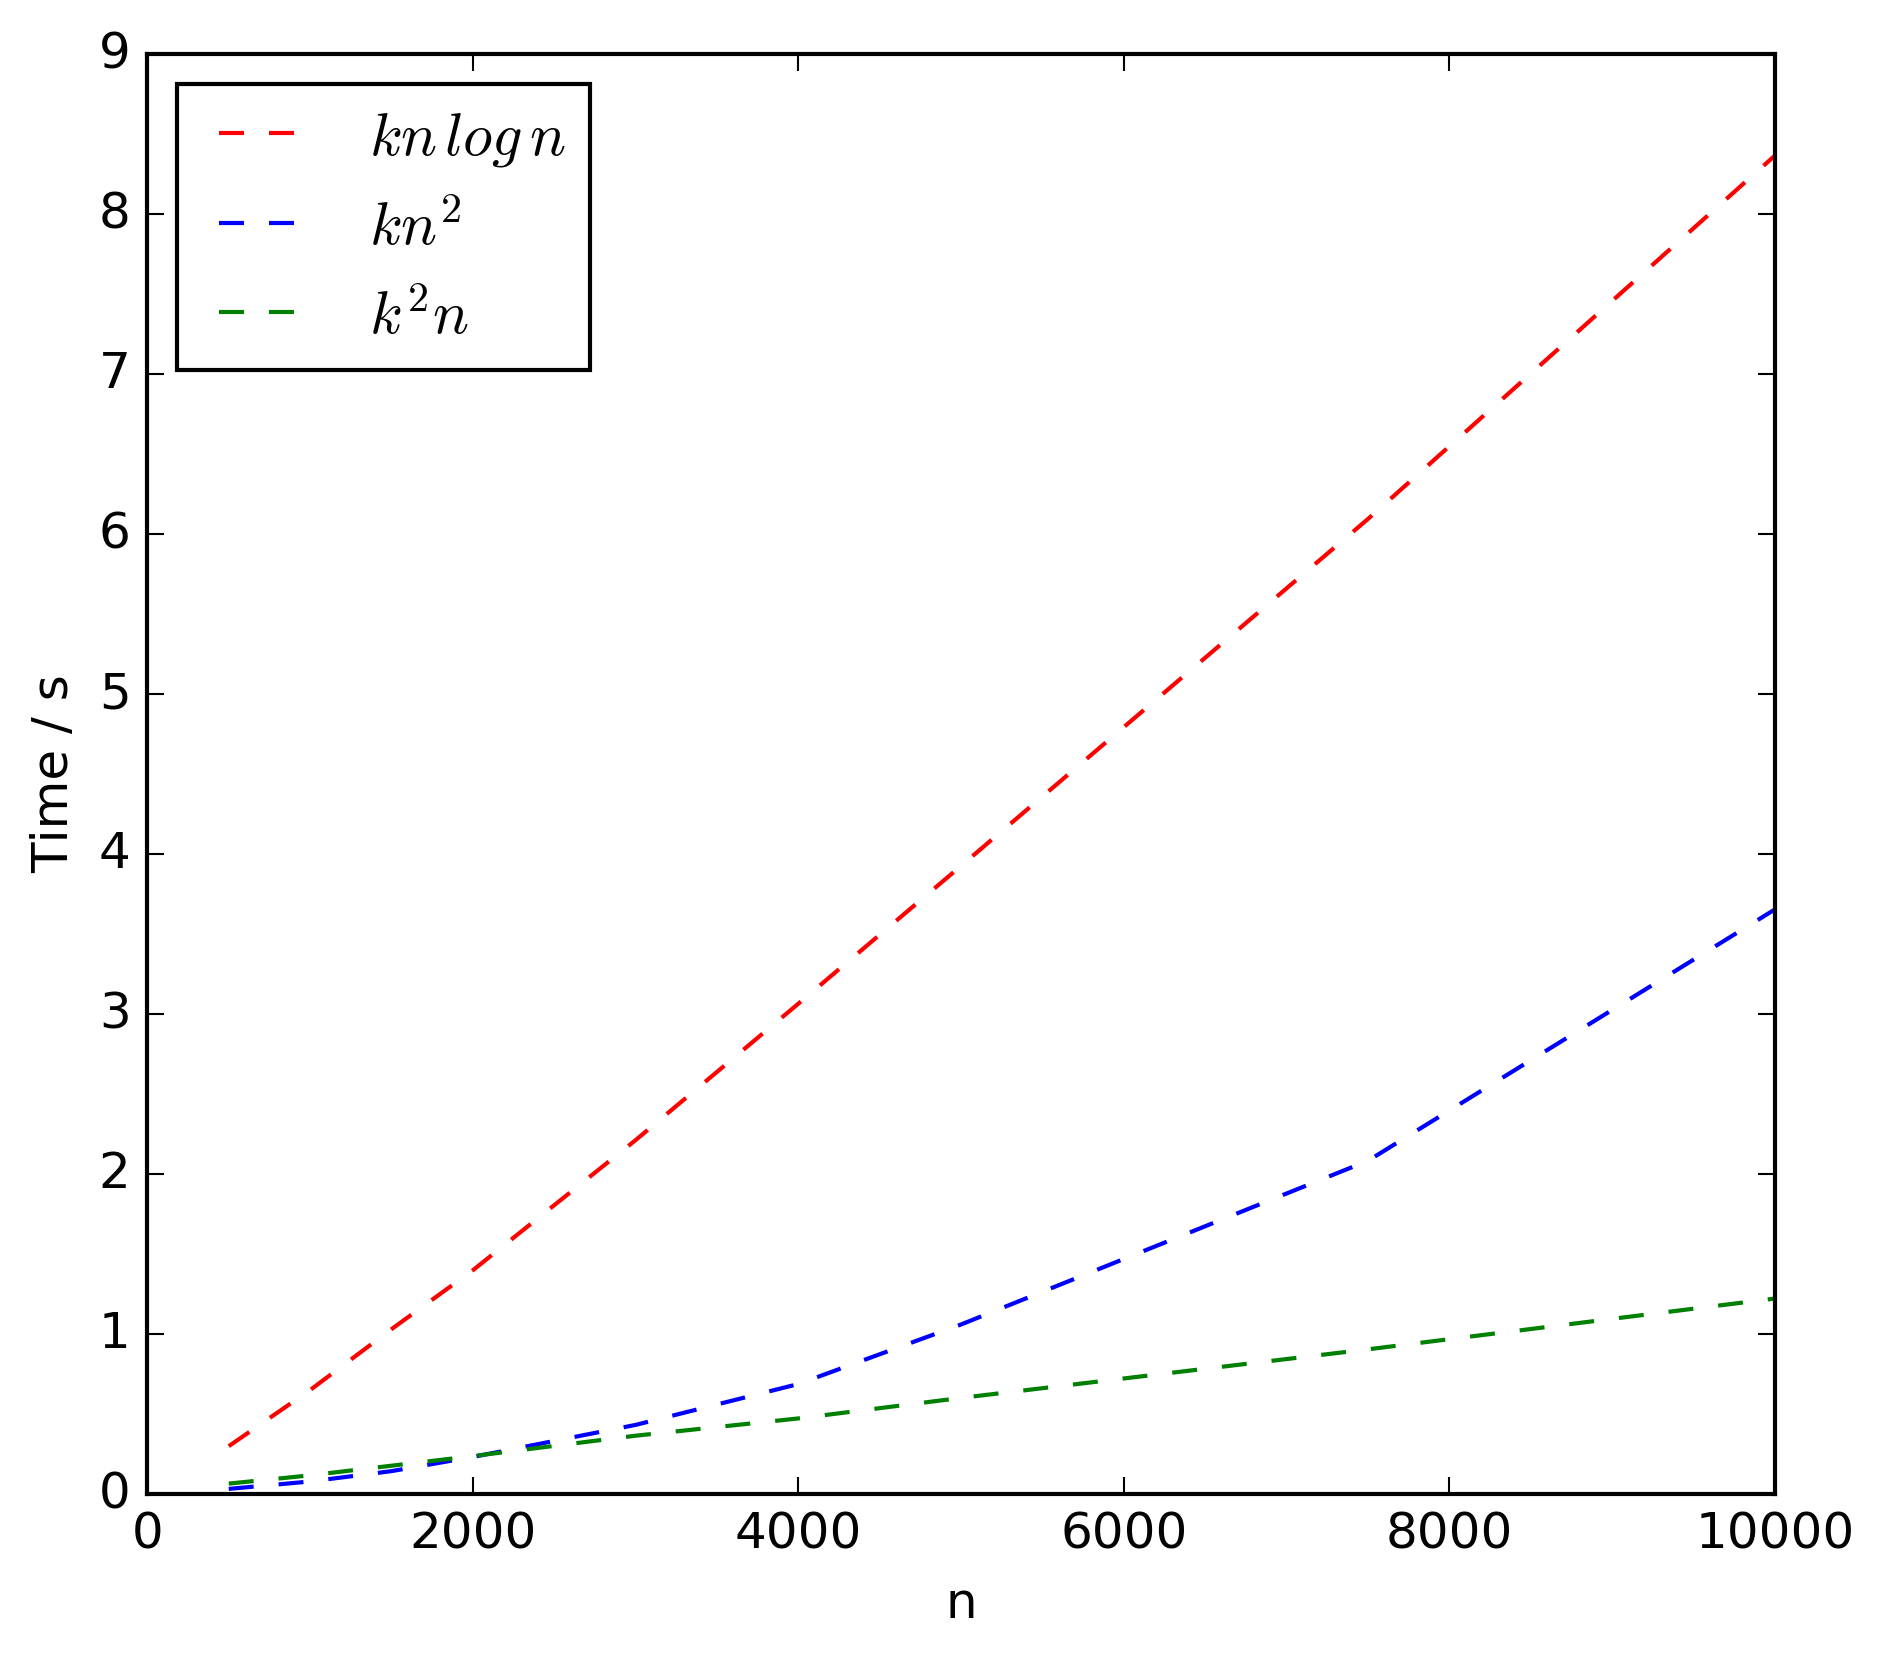
\includegraphics[scale=0.4]{varyingn1_weighting}
        \end{minipage}\hfill
        \begin{minipage}{0.48\textwidth}
            \centering
            \caption[Runtime of \texttt{Filter\_Clusters} in Scenario 1, with $k = 100$ and varying $n$]{\texttt{Filter\_Clusters} time with $k = 100$, varying $n$}
            \label{tab:filtern1}
            \begin{tabular}{c||ccccc}
                $n$ & $n\,log\,n$ & $n\,log^2n$\\
                \hline\hline
                500 & 1.09 & 0.51\\
                1000 & 2.22 & 2.42\\
                1500 & 3.33 & 10.86\\
                2000 & 4.54 & 17.74\\
                3000 & 7.06 & 31.29\\
                4000 & 9.62 & 49.92\\
                5000 & 12.20 & 69.88\\
                7500 & 18.54 & 129.07\\
                10000 & 25.38 & 211.64\\
            \end{tabular}
            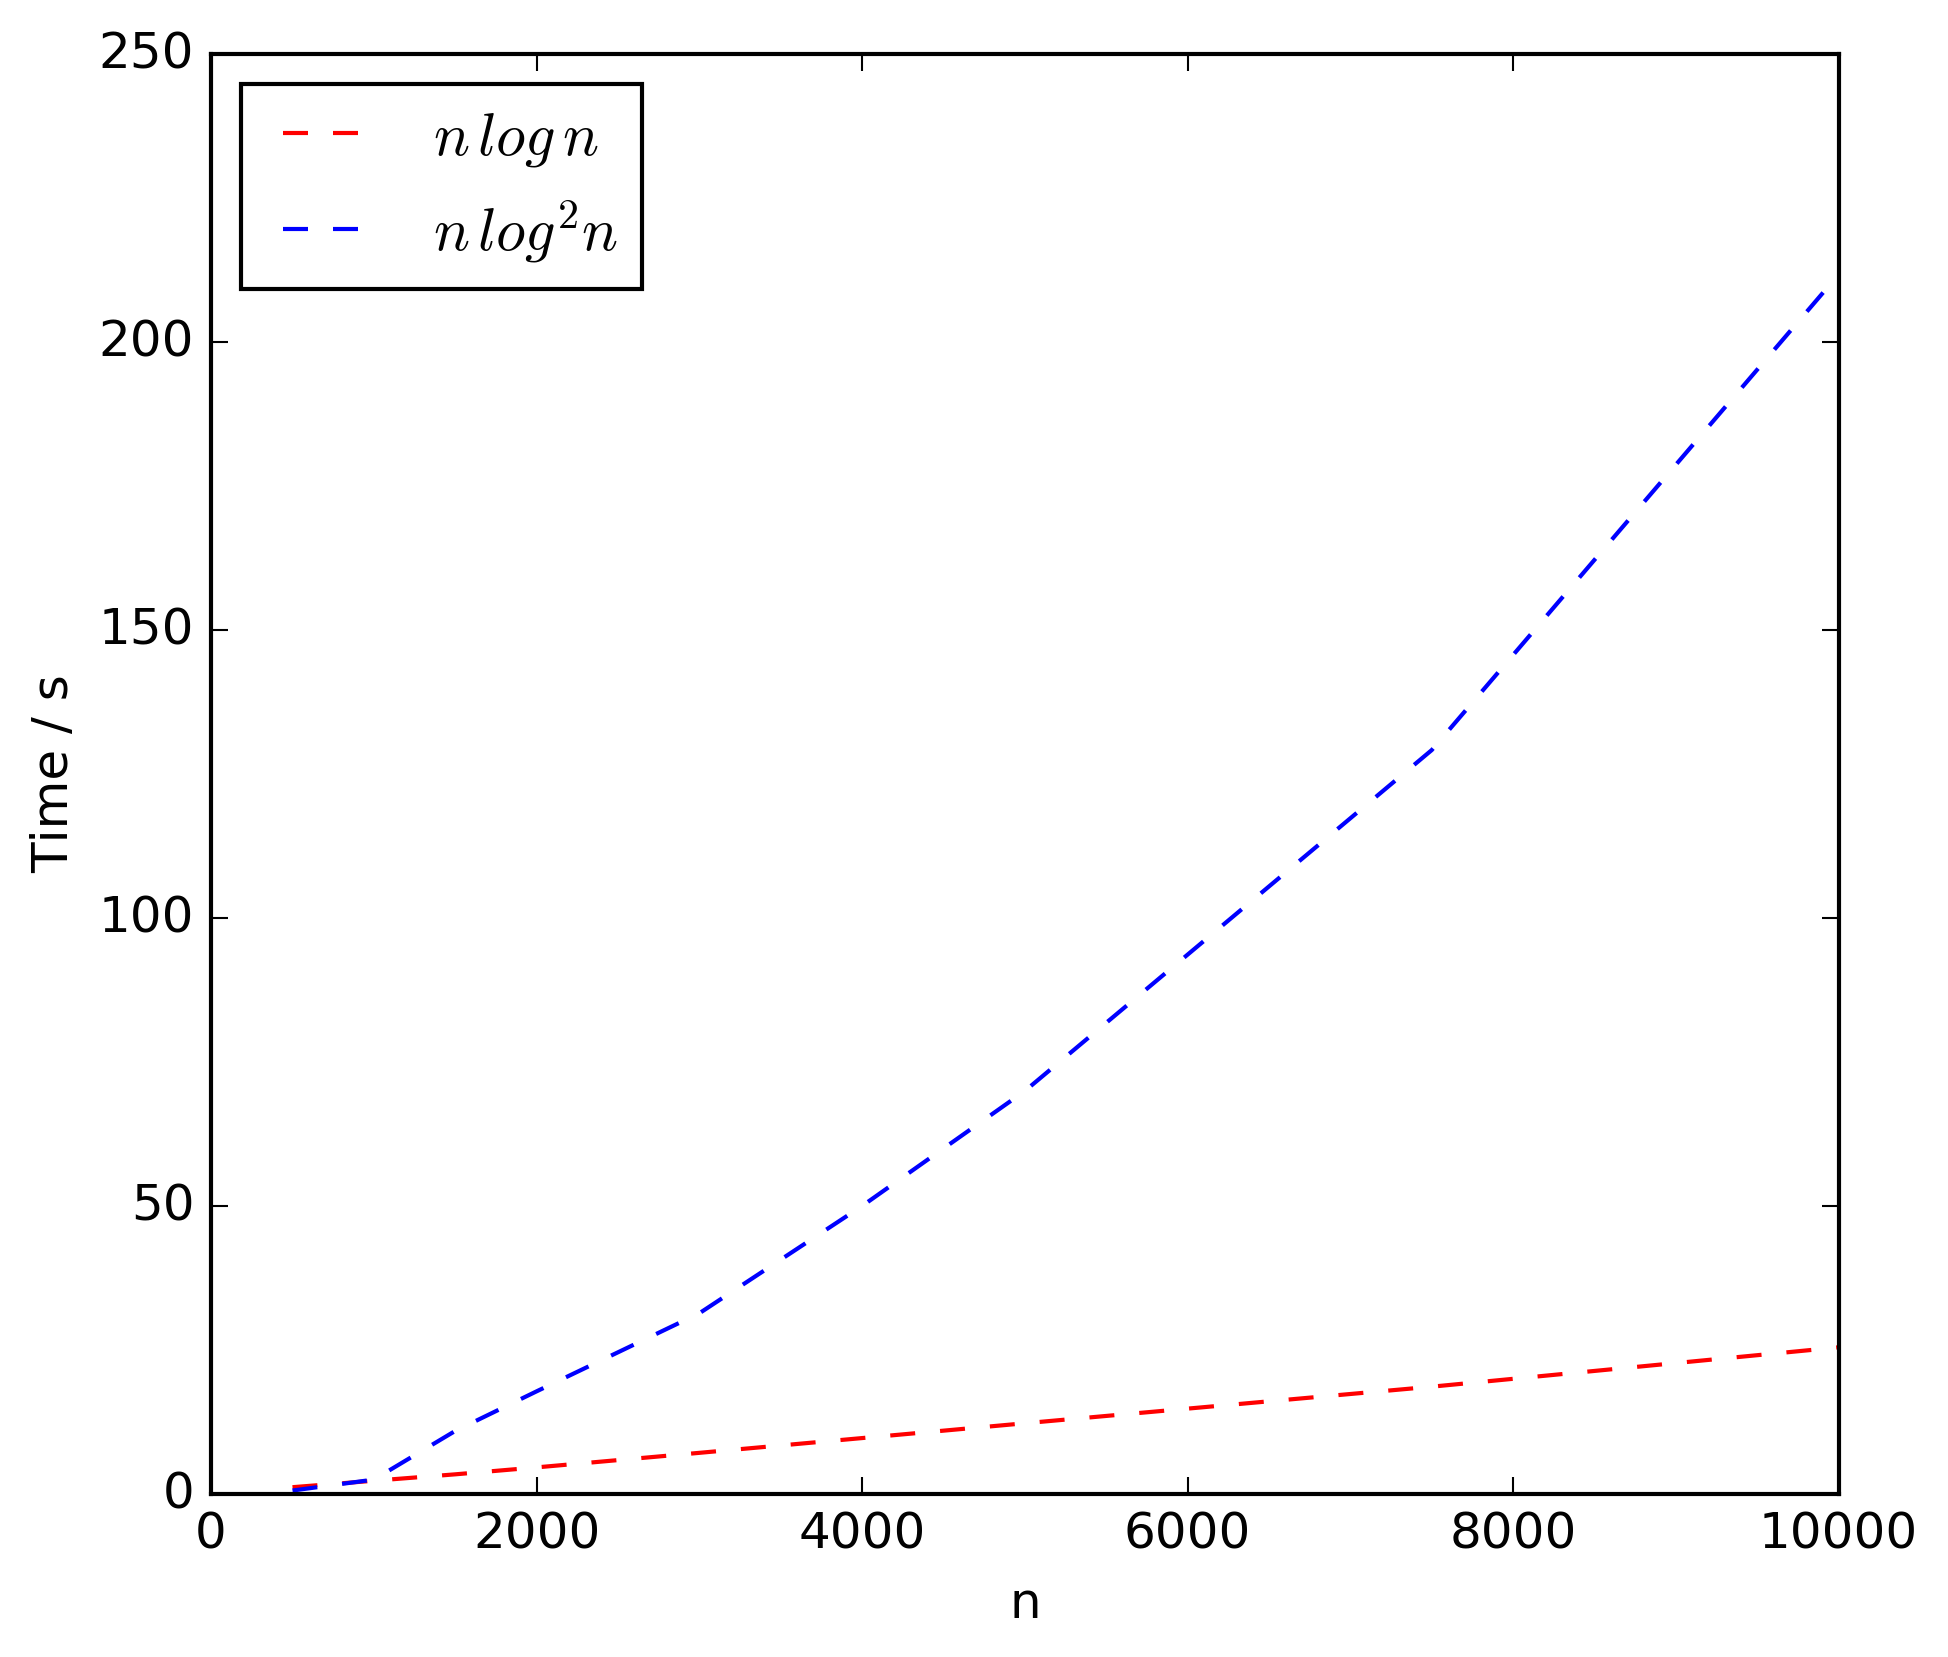
\includegraphics[scale=0.4]{varyingn1_filter}
        \end{minipage}
        \captionof{figure}{Experimental Results for Scenario $1$}
        \label{fig:expresults1}
    \end{table}

    \begin{table}[!ht]
        \captionsetup{font=footnotesize,justification=centering,margin=0cm}
        \fontsize{9}{11}\selectfont
        \begin{minipage}{0.48\textwidth}
            \centering
            \caption[Runtime of the Weighting step in Scenario 2, with $n = 1000$ and varying $k$]{Weighting time with $n = 1000$, varying $k$}
            \label{tab:weightk2}
            \begin{tabular}{c||ccccc}
                $k$ & $kn\,log\,n$ & $kn^2$ & $k^2n$\\
                \hline\hline
                50 & 0.41 & 0.04 & 0.03\\
                100 & 0.80 & 0.08 & 0.10\\
                200 & 1.57 & 0.18 & 0.37\\
                500 & 4.10 & 0.50 & 2.29\\
                1000 & 8.62 & 1.09 & 8.95\\
                2000 & 17.56 & 2.39 & 35.30\\
                3000 & 27.30 & 3.71 & 79.17\\
                4000 & 37.71 & 5.16 & 140.47\\
            \end{tabular}
            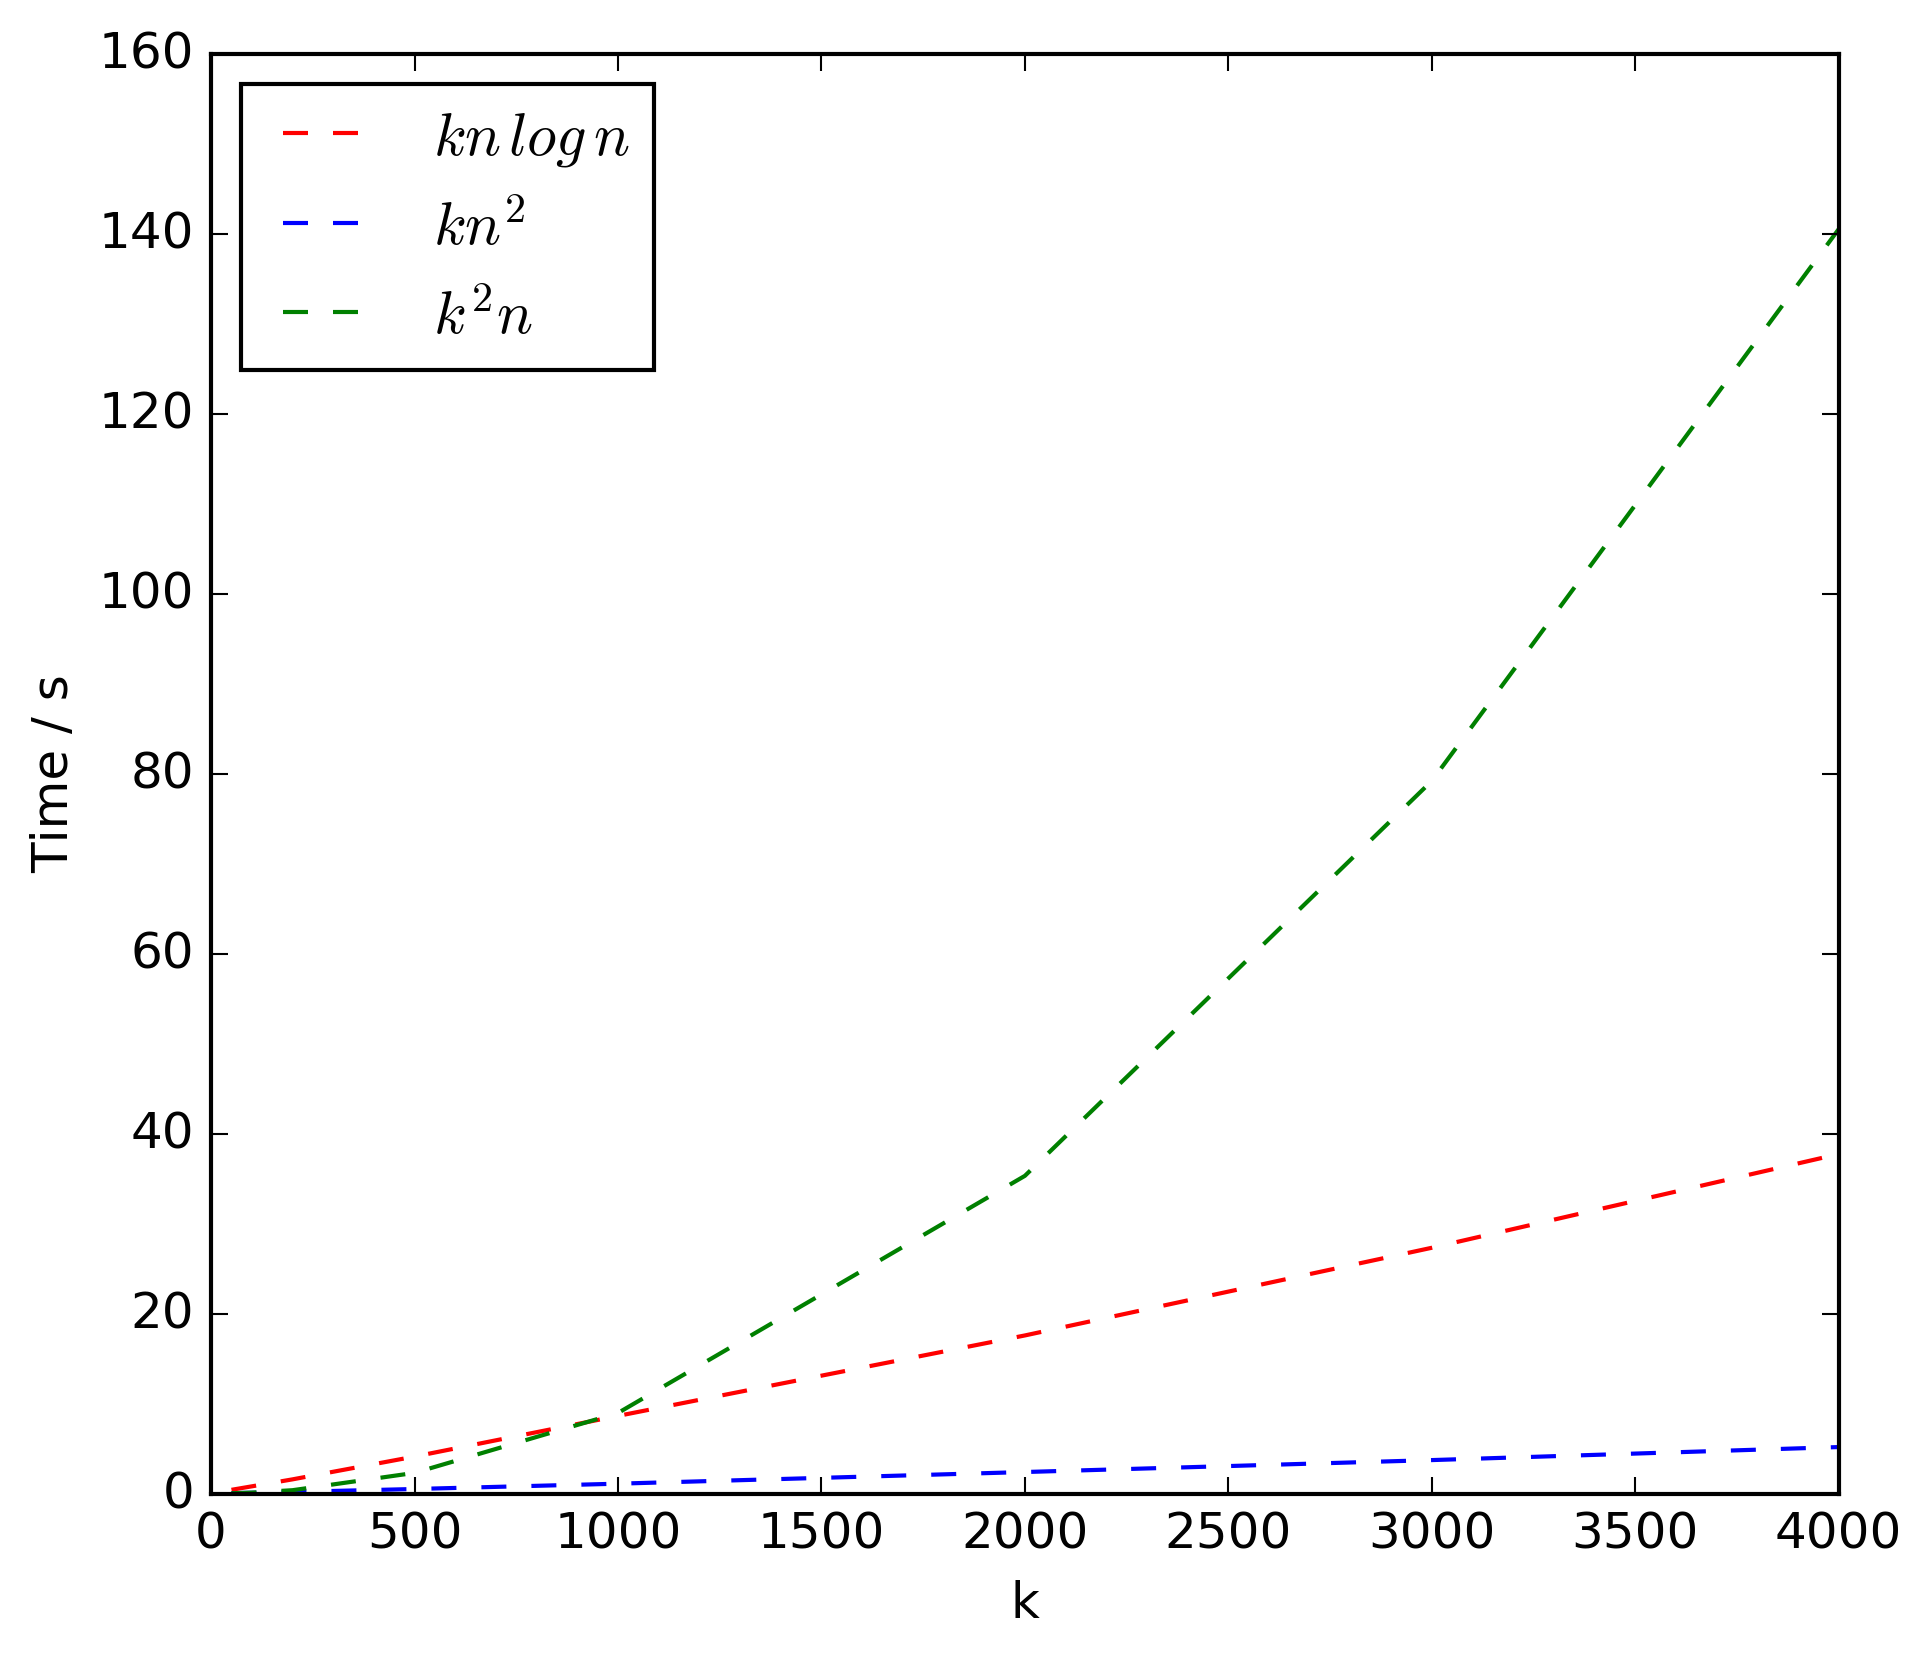
\includegraphics[scale=0.4]{varyingk2_weighting}
            \vspace{0.5cm}
        \end{minipage}\hfill
        \begin{minipage}{0.48\textwidth}
            \centering
            \caption[Runtime of \texttt{Filter\_Clusters} in Scenario 2, with $n = 1000$ and varying $k$]{\texttt{Filter\_Clusters} time with $n = 1000$, varying $k$}
            \label{tab:filterk2}
            \begin{tabular}{c||ccccc}
                $k$ & $n\,log\,n$ & $n\,log^2n$\\
                \hline\hline
                50 & 1.14 & 1.00\\
                100 & 2.18 & 2.78\\
                200 & 4.38 & 5.54\\
                500 & 11.24 & 19.86\\
                1000 & 22.87 & 46.90\\
                2000 & 49.79 & 101.64\\
                3000 & 80.24 & 162.47\\
                4000 & 112.12 & 227.85\\
            \end{tabular}
            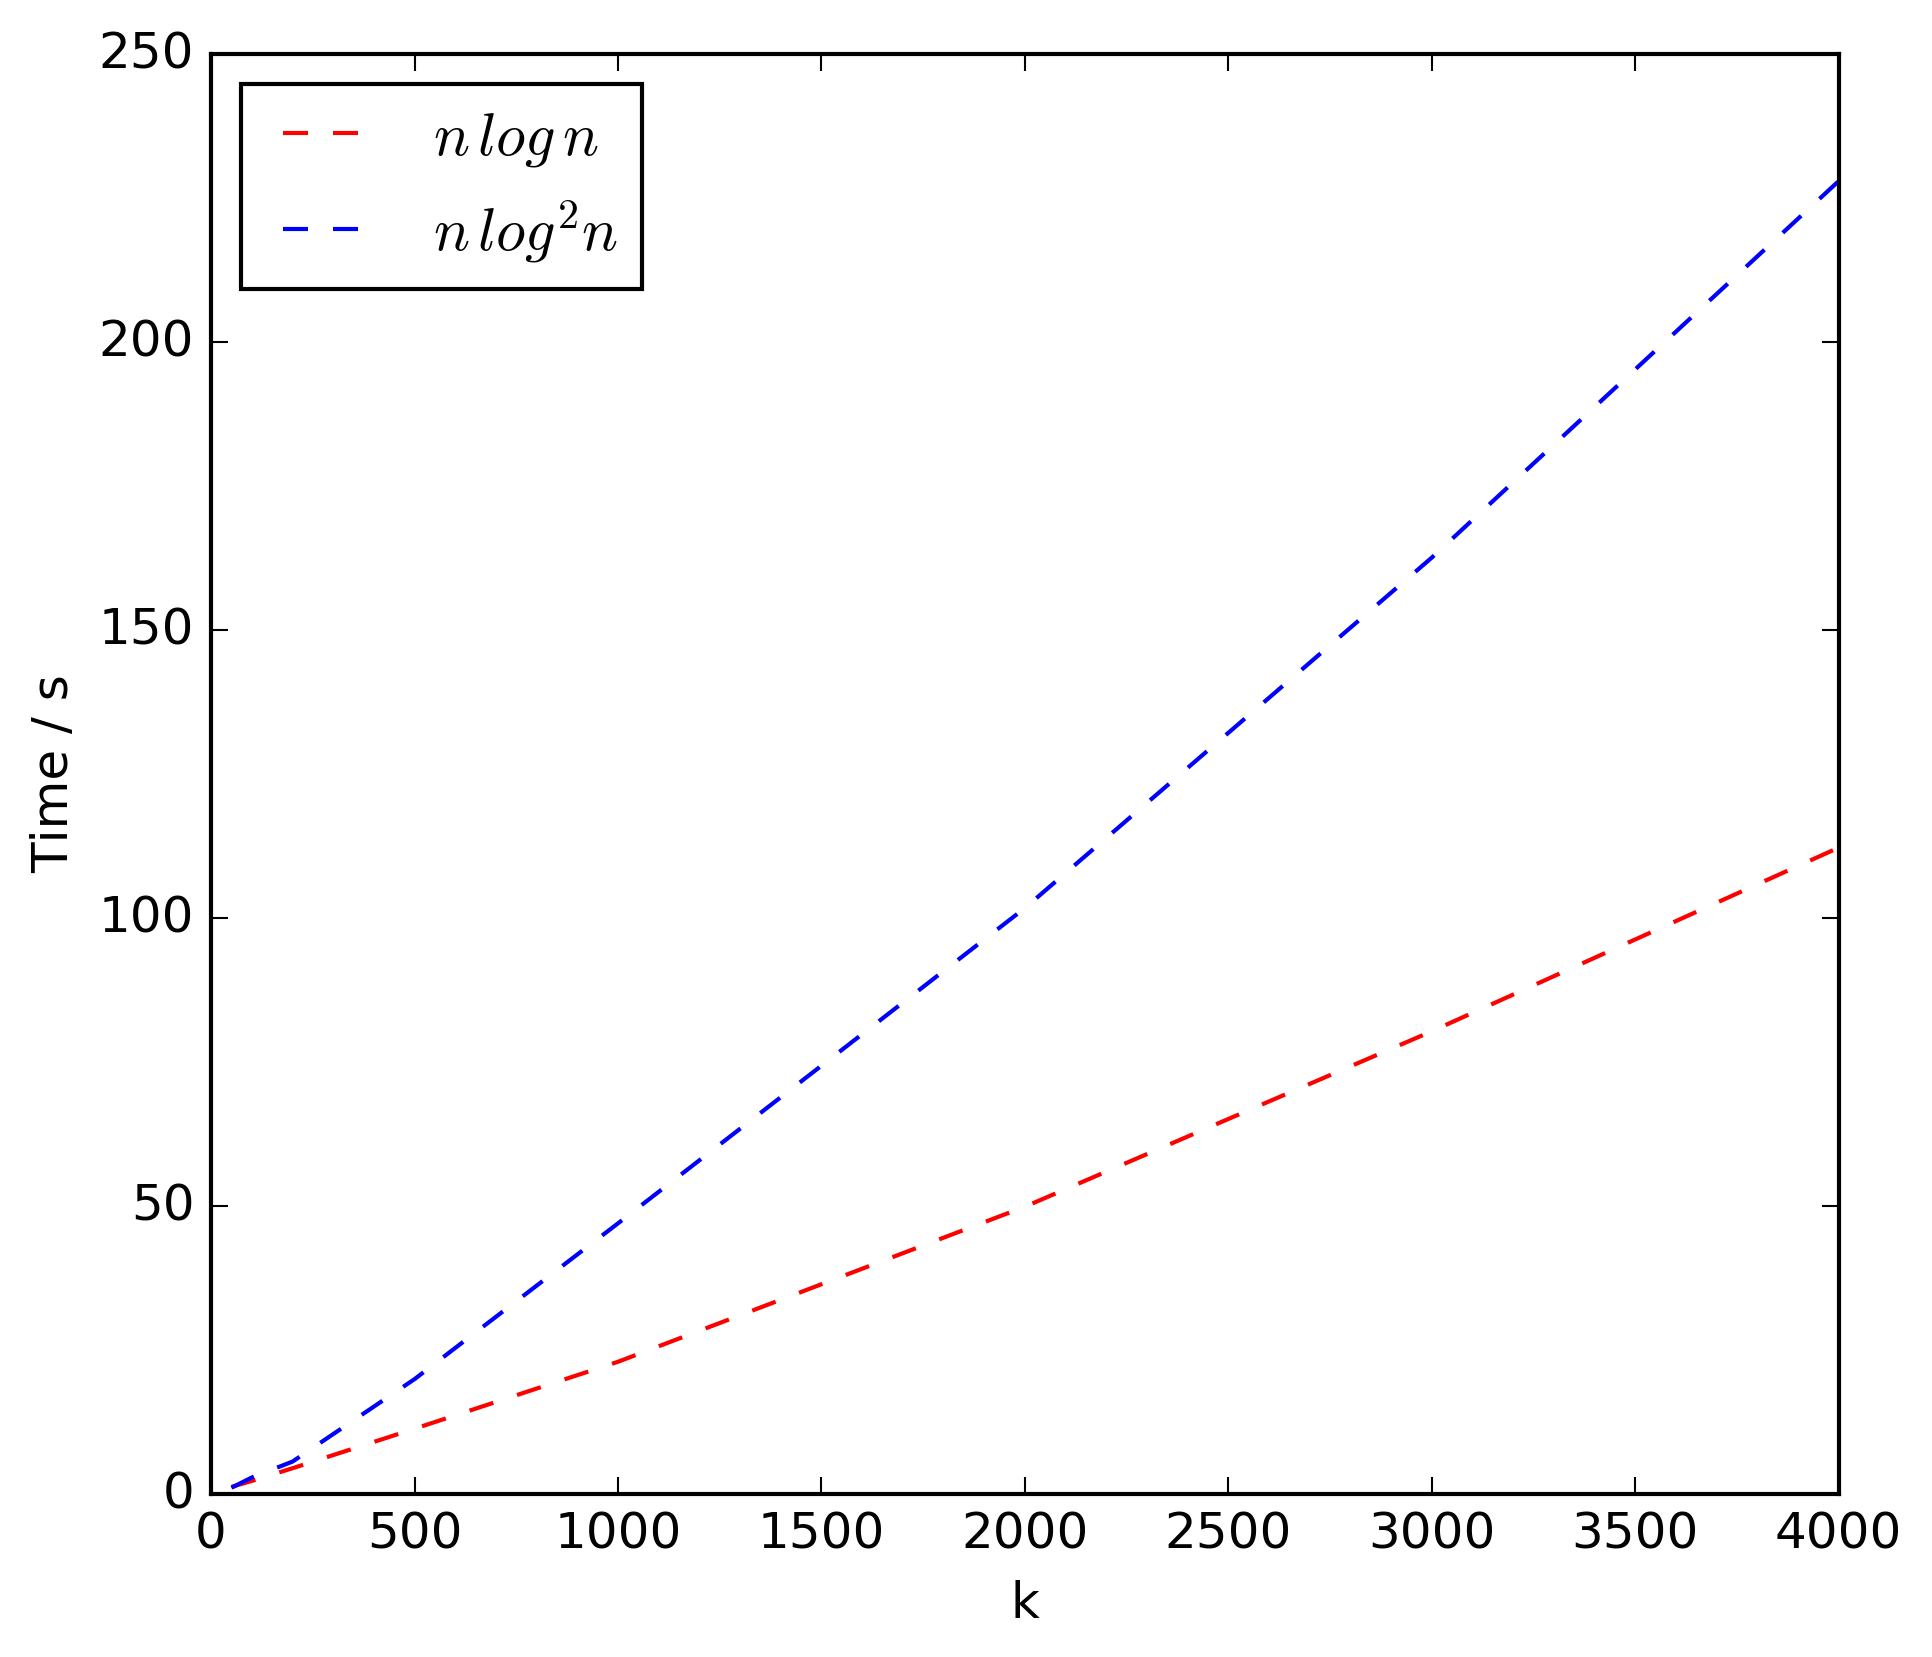
\includegraphics[scale=0.4]{varyingk2_filter}
            \vspace{0.5cm}
        \end{minipage}
        \begin{minipage}{0.48\textwidth}
            \centering
            \caption[Runtime of the Weighting step in Scenario 2, with $k = 100$ and varying $n$]{Weighting time with $k = 100$, varying $n$}
            \label{tab:weightn2}
            \begin{tabular}{c||ccccc}
                $n$ & $kn\,log\,n$ & $kn^2$ & $k^2n$\\
                \hline\hline
                1000 & 0.75 & 0.08 & 0.09\\
                2000 & 1.68 & 0.25 & 0.20\\
                3000 & 2.68 & 0.43 & 0.29\\
                5000 & 4.77 & 1.05 & 0.48\\
                7500 & 7.56 & 2.07 & 0.76\\
                10000 & 10.59 & 3.62 & 1.01\\
                20000 & 24.49 & 11.11 & 2.08\\
                30000 & 37.76 & 28.42 & 3.18\\
                40000 & 53.57 & 73.68 & 4.42\\
            \end{tabular}
            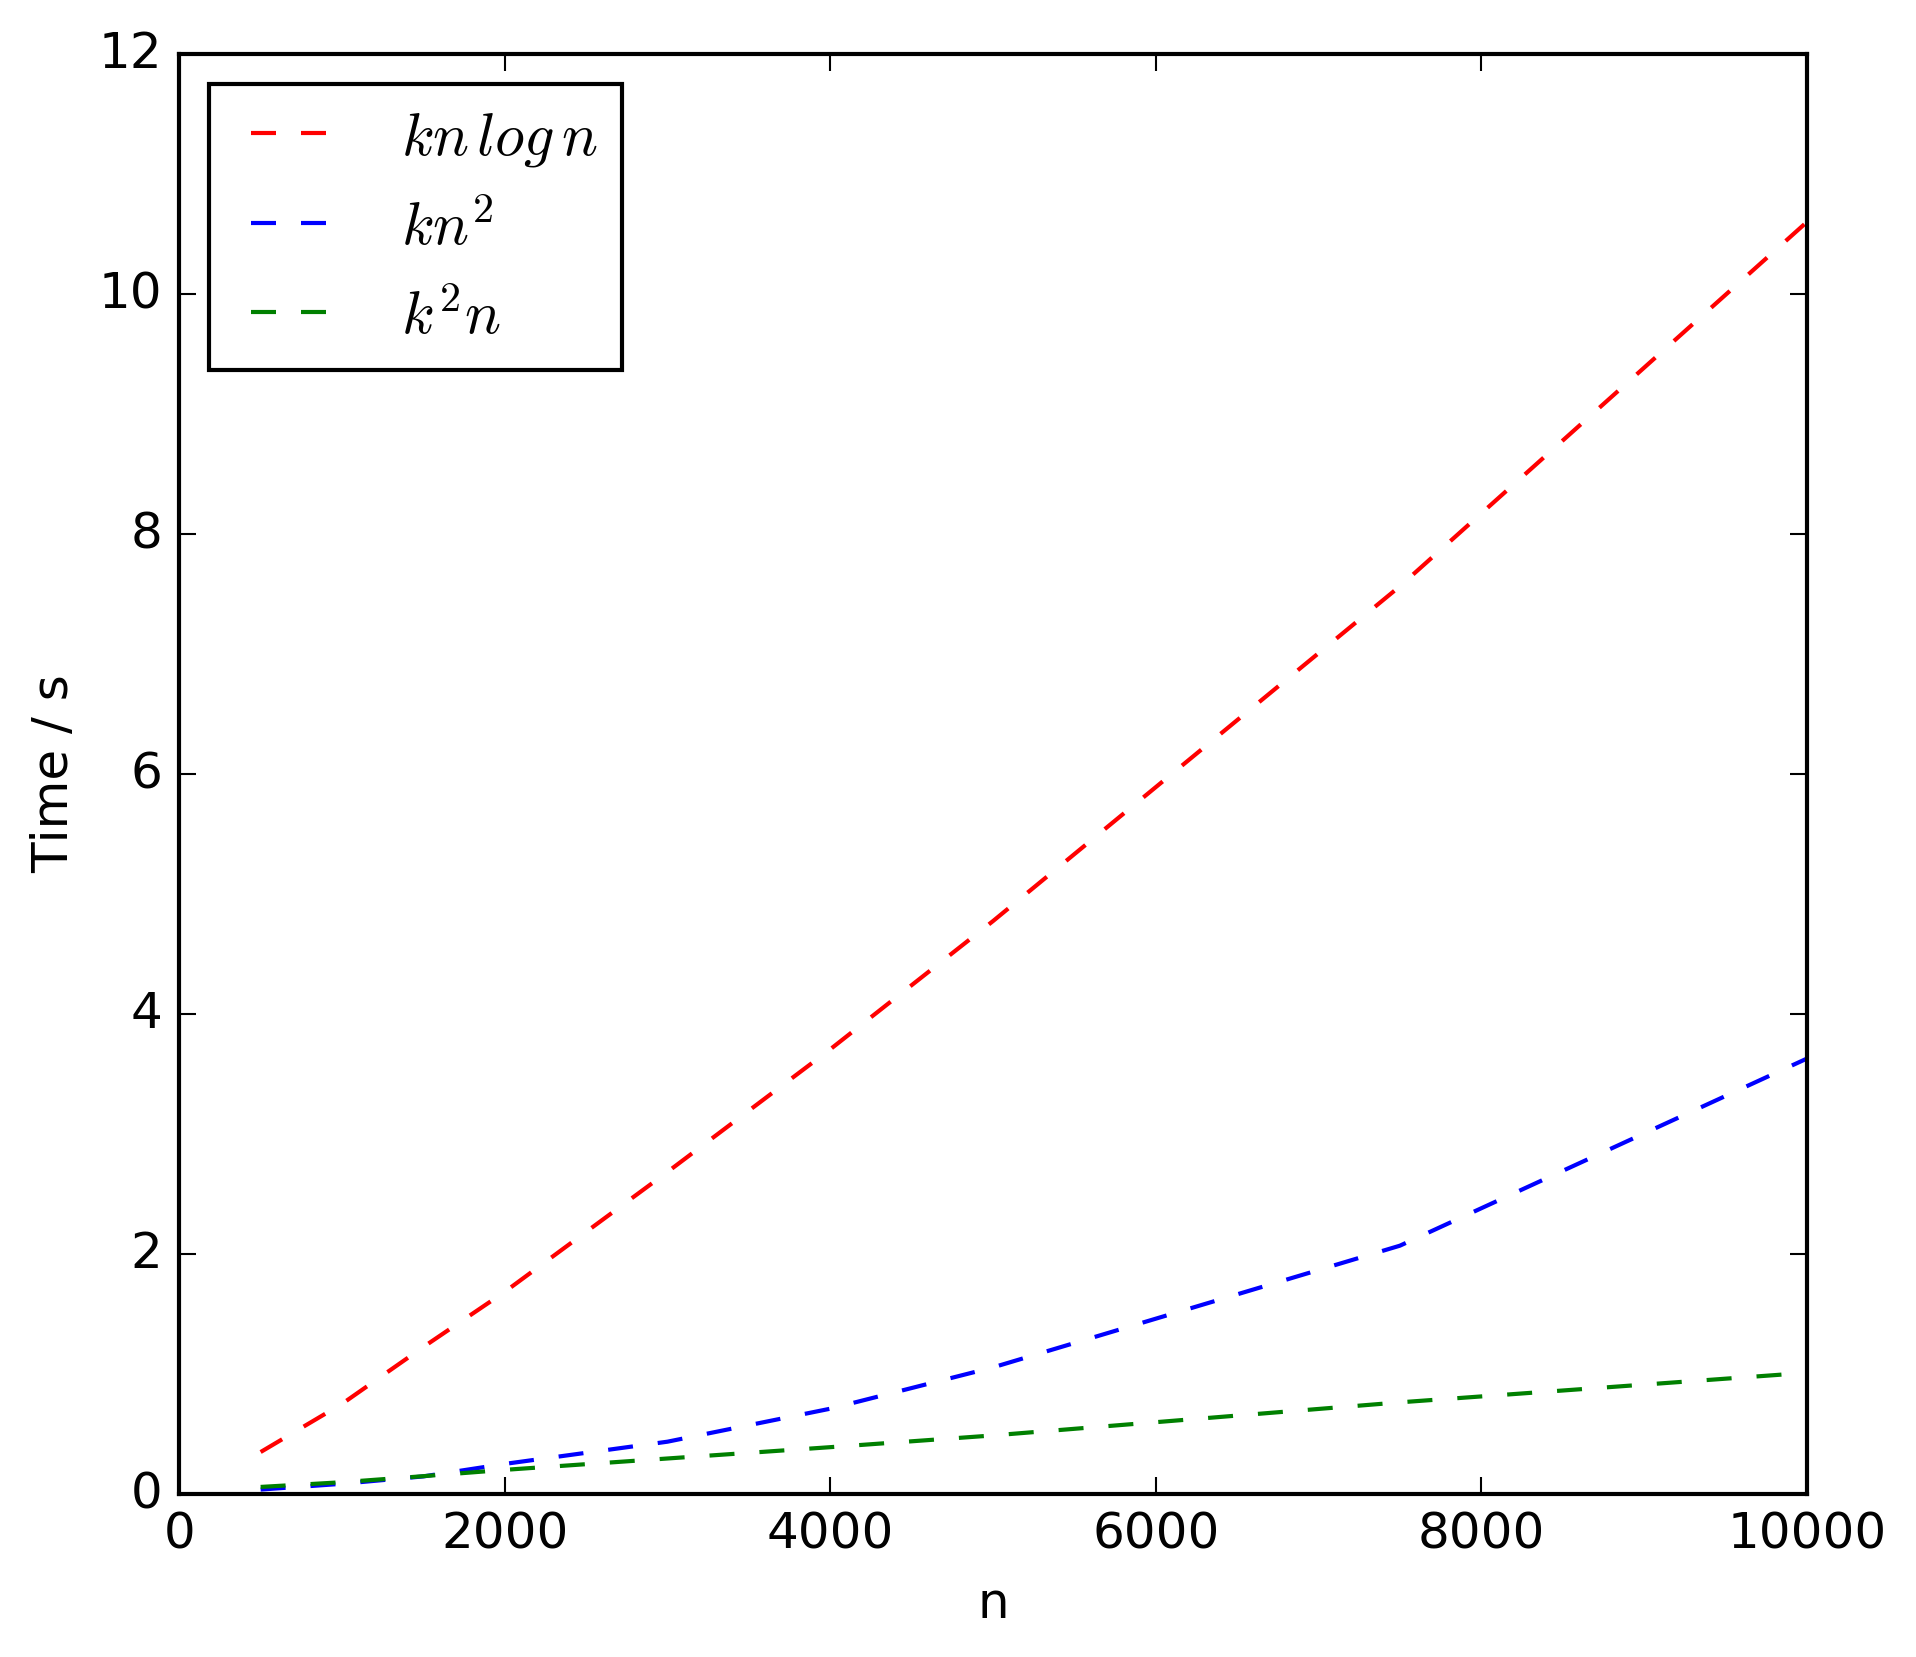
\includegraphics[scale=0.4]{varyingn2_weighting}
        \end{minipage}\hfill
        \begin{minipage}{0.49\textwidth}
            \centering
            \caption[Runtime of \texttt{Filter\_Clusters} in Scenario 2, with $k = 100$ and varying $n$]{\texttt{Filter\_Clusters} time with $k = 100$, varying $n$}
            \label{tab:filtern2}
            \begin{tabular}{c||ccccc}
                $n$ & $n\,log\,n$ & $n\,log^2n$\\
                \hline\hline
                500 & 1.04 & 0.60\\
                1000 & 2.09 & 2.65\\
                1500 & 3.20 & 7.34\\
                2000 & 4.40 & 11.84\\
                3000 & 6.77 & 20.64\\
                4000 & 9.28 & 32.04\\
                5000 & 11.81 & 45.94\\
                7500 & 18.71 & 90.62\\
                10000 & 26.69 & 150.22\\
            \end{tabular}
            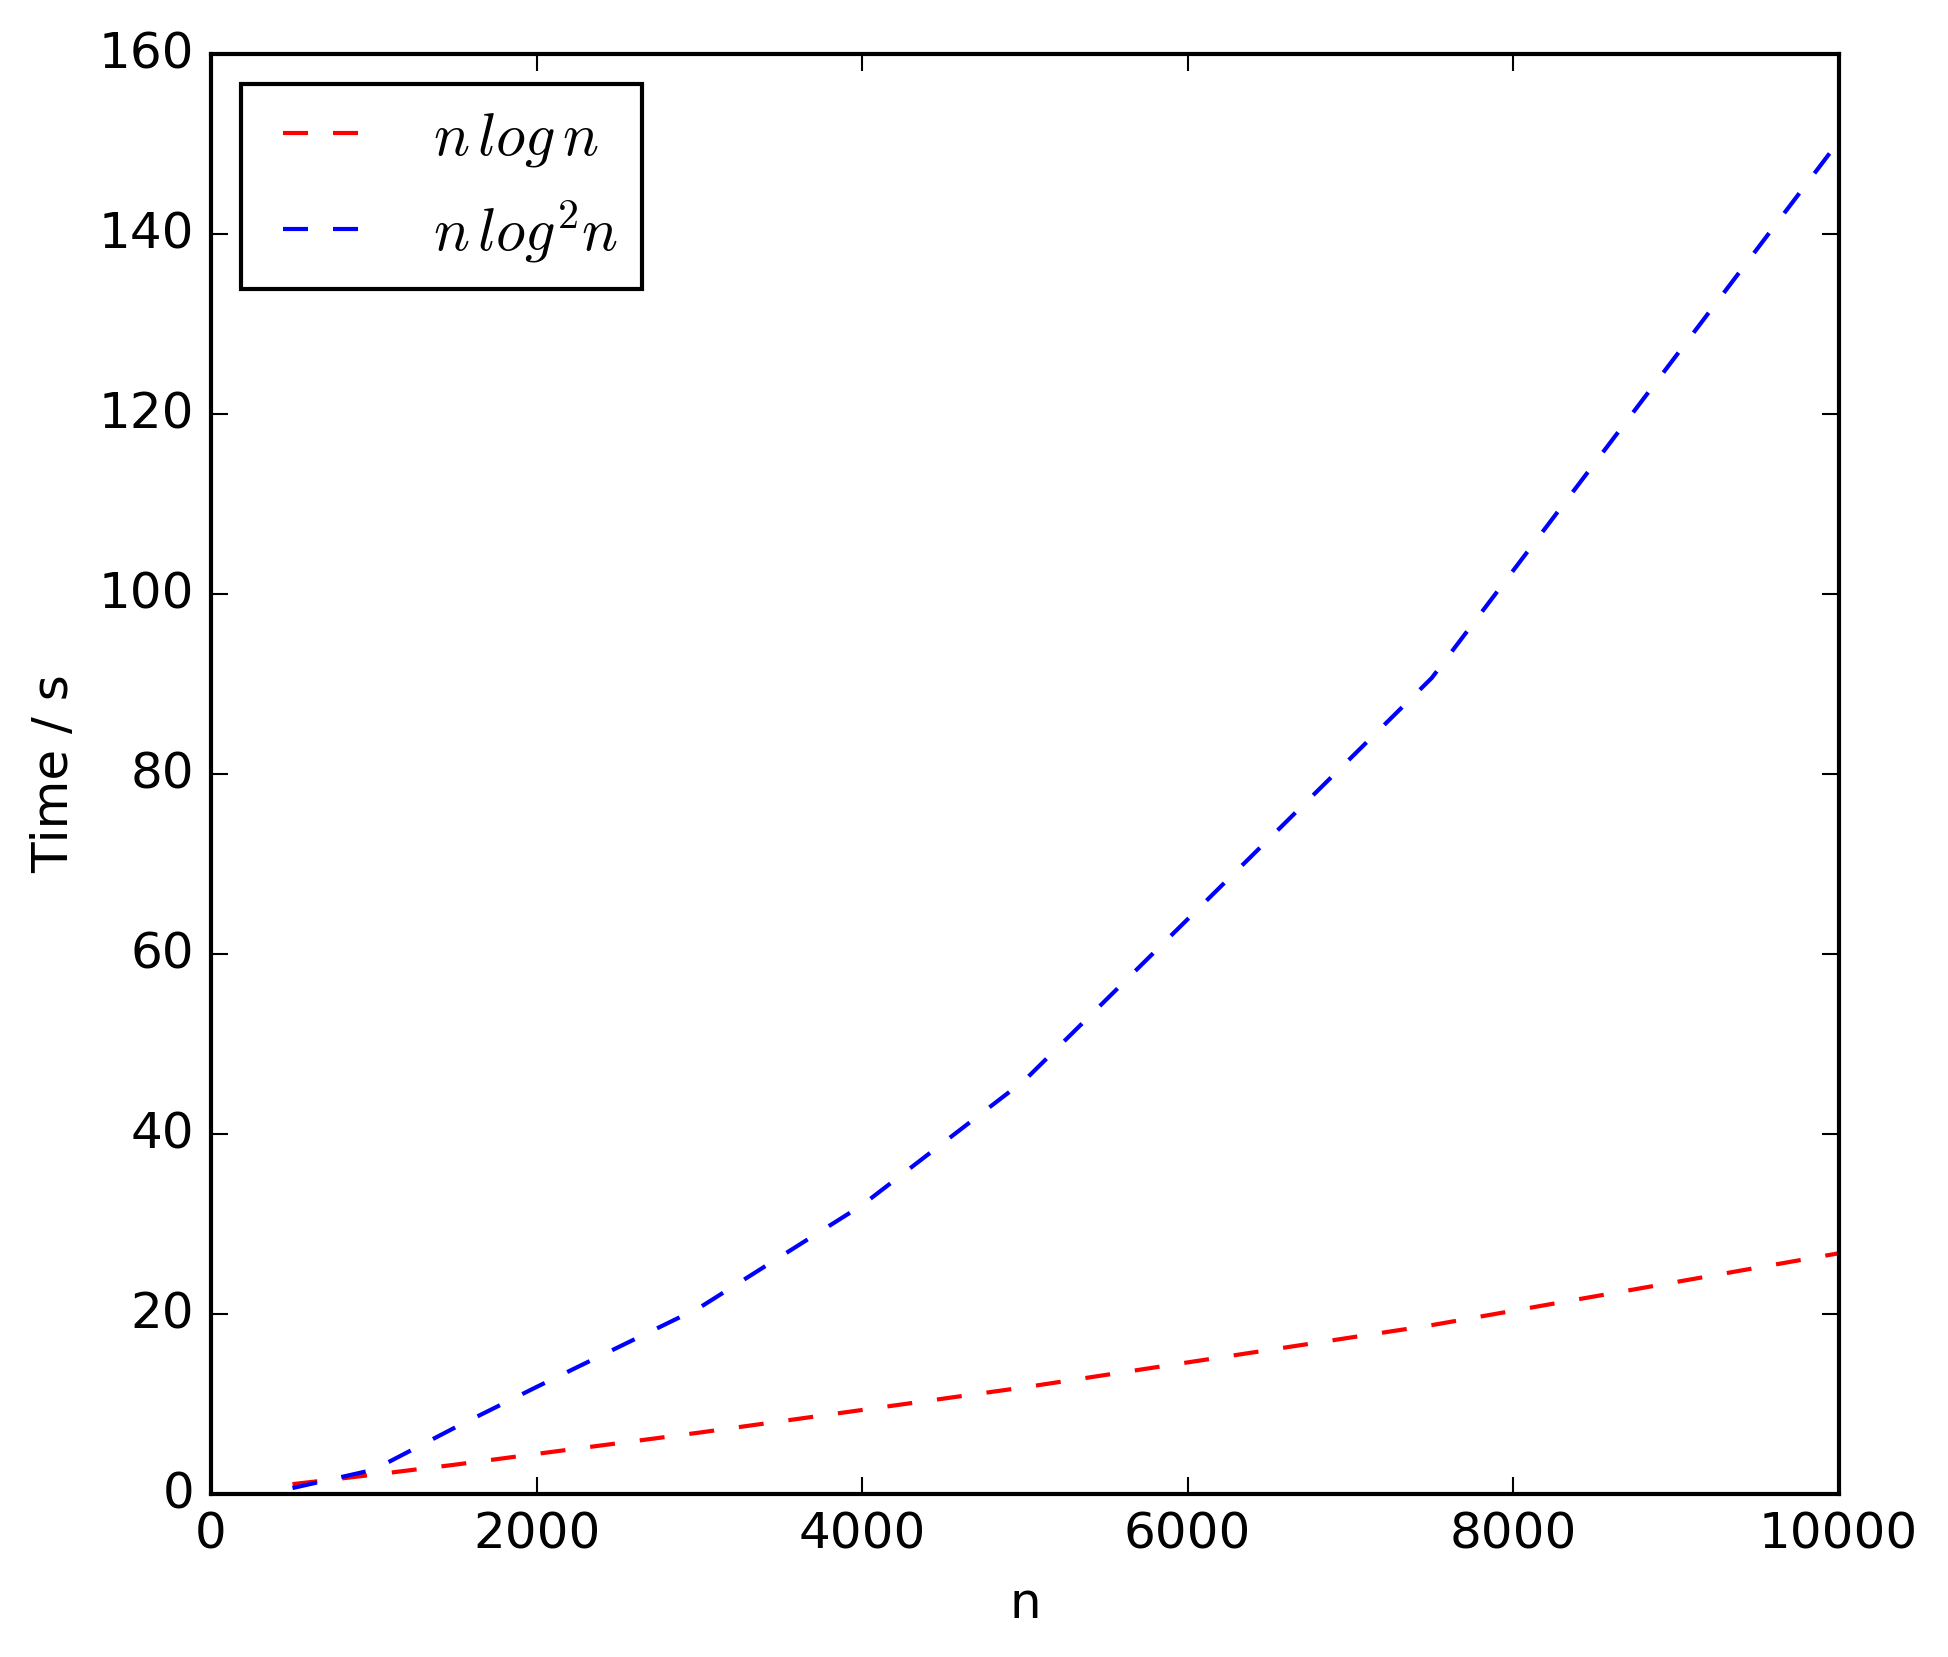
\includegraphics[scale=0.4]{varyingn2_filter}
        \end{minipage}
        \captionof{figure}{Experimental Results for Scenario $2$}
        \label{fig:expresults2}
    \end{table}

    The experimentally observed average running times are given in \cref{tab:weightk1,tab:filterk1,tab:weightn1,tab:filtern1,tab:weightk2,tab:filterk2,tab:weightn2,tab:filtern2}, seen in \cref{fig:expresults1,fig:expresults2}.

    \textit{Comparing Scenarios.} Observe that the basic structure of the graphs across the two scenarios is the same, i.e. we see the same relationships between the various algorithms. An interesting case is to compare Table~\ref{tab:weightn1} to Table~\ref{tab:weightn2}. It can be seen from these that the $kn\,log\,n$ weighting algorithm performs worse in Scenario 2. This is likely because in Scenario 2 there is a far larger number of distinct clusters, increasing the range of the labels assigned during the weighting step. This leads to the counting/radix sorts becoming less efficient. It can also be seen that the $n\,log^2n$ \texttt{Filter\_Clusters} algorithm performs differently in the two scenarios. Specifically, when we vary $n$, it performs better in Scenario 2 (compare Tables~\ref{tab:filtern1} and~\ref{tab:filtern2}). As pointed out in \cite{jansson2018algorithms}, this is because the larger number of distinct clusters in Scenario 2 leads to more clusters being discarded due to the filtering, due to which the algorithm needs to maintain a smaller tree. We can also see that it performs worse in Scenario 2 when we vary $k$ (compare Tables~\ref{tab:filterk1} and~\ref{tab:filterk2}). To explain this, we note that this implementation in fact uses a simpler version of \texttt{Filter\_Clusters}, with time complexity $O(n^2)$, when $n \leq 1000$. The runtime of this algorithm increases as the number of incompatible nodes increases, and hence it performs worse under Scenario 2. Since our algorithm performs similarly for both scenarios, apart from the discussion above, we will henceforth only be referring to \cref{tab:weightk1,tab:filterk1,tab:weightn1,tab:filtern1}.

    \textit{Weighting Step.} From Table~\ref{tab:weightk1}, it is clear that, as expected, as $k$ increases, the runtime of the $k^2n$ algorithm becomes much worse than that of the other two. Similarly, Table~\ref{tab:weightn1} shows that when $n$ increases, runtime of the $kn^2$ becomes worse than that of the $k^2n$. More interestingly, the algorithm with a theoretical runtime of $kn\,log\,n$ actually performs worse than the $kn^2$ one for values of $n$ up to around $25000$. This is because the constants in the new algorithm are larger, due to the construction of the restricted subtrees. However, we can see that the runtime for the $kn^2$ algorithm is growing faster than the new algorithm, and it does indeed perform worse for very large values of $n$. In practice, though, values of $n$ are not so large, and hence it is likely that the old implementation is better in practice. Also note that, as mentioned in \cite{jansson2018algorithms}, the $kn^2$ algorithm costs memory quadratic in $n$, so if memory is a concern, then using on of the other methods might be more advisable. The choice of which one to use would depend on the value of $k$.

    \texttt{Filter\_Clusters.} Table~\ref{tab:filterk1} is not particularly interesting here since it merely demonstrates that the two algorithms perform similarly when $n = 1000$. However, Table~\ref{tab:filtern1} illustrates that the new algorithm overtakes the old one very quickly when $n > 1000$, performing up to $10$ times better as $n$ nears $10000$. This might be surprising, as the theoretical difference is only a factor of $log\,n$. We (informally) think that this is because of implementation detail 3, due to which we can skip the costly construction of the $\TB||\leafset^{\tau}$ trees. Thus, based on these results, we recommend using the old algorithm if $n \leq 1000$ and the new one otherwise. Note that this would in fact mean using the simpler version of \texttt{Filter\_Clusters}, with time complexity $O(n^2)$, when $n \leq 1000$.

    \section{Conclusion}
    We have given a new deterministic algorithm for constructing the FDCT of a set of phylogenetic trees. This algorithm betters the previously best known one by a factor of $log\,n$. We leave open the problem of finding an optimal solution, i.e. one with time complexity $O(kn)$. Observe that doing so would involve bettering both halves of the algorithm or coming up with a new approach.

    \newpage
    \bibliographystyle{apacite}
    \bibliography{final_report}
\end{document}
